\chapter{حمله‌های جبری و روش‌های حل دستگاه معادلات چندجمله‌ای}
در بخش قبل نشان دادیم که مسئله‌ی شکستن سامانه‌ی رمزنگاری را می‌توان به مسئله‌ی حل دستگاه معادلات چندجمله‌ای تبدیل کرد و معادلات حاکم بر چند سامانه‌ی واقعی را نیز استخراج کردیم. بنابراین اگر بتوان الگوریتم مناسبی برای حل دستگاه معادلات چندجمله‌ای یافت آن‌گاه امنیت تمام سامانه‌های رمزنگاری با خطر مواجه می‌شود. به همین خاطر در این فصل به معرفی الگوریتم‌هایی می‌پردازیم که رمزنگارها غالباً از آن‌ها برای حل دستگاه‌های به‌دست آمده از سامانه‌های رمزنگاری استفاده می‌کنند. بخش عمده‌ای از مطالب این فصل بر پایه‌ی مراجع 
\cite{bard2009algebraic, courtois2000efficient, cca2_kreuzer}
و
\cite{albrecht2010alorithmic, courtois2002cryptanalysis, ullah2012new}
است.



\section{روش‌های مبنی بر خطی سازی}
\subsection{خطی سازی}
در روش خطی‌سازی به‌جای هر یکجمله‌ای یک متغیر جدید جایگزین می‌کنیم، با این‌ کار دستگاه معادلات چندجمله‌ای به یک دستگاه خطی بر حسب متغیرهای جدید تبدیل می‌شود. دستگاه خطی با روش حذفی گاوس به سرعت قابل حل است. روش خطی سازی گرچه خیلی ساده است، ولی یکی از مراحل اصلی در حمله‌هایی است که در ادامه معرفی می‌کنیم. 
\begin{example}
دستگاه معادلات زیر روی میدان 
$\ffld_{7}$
را در نظر بگیرید. 
	$$\left \{ \begin{array}{l}
	x_{1}+x_{2}+x_{1}x_{2} = 1\\
	x_{2}+x_{1}x_{2} = 1\\
	x_{1}+x_{1}x_{2} = 0
	\end{array} \right.$$

با جایگزینی‌های 
$y_{1} = x_{1}$
و
$y_{2} = x_{2}, y_{12} =  x_{1}x_{2}$
به دستگاه خطی زیر می‌رسیم.
	$$\left \{ \begin{array}{l}
	y_{1}+y_{2}+y_{12} = 1\\
	y_{2}+y_{12} = 1\\
	y_{1}+y_{12} = 0
	\end{array} \right.$$
با حل دستگاه فوق داریم:
	$$\left\{ y_{1}=0,y_{12}=0,y_{2}=1 \right\} \Longrightarrow \{x_{1} = 0, x_{2} = 1\}.$$
\end{example}
بدیهی است که هر جواب از دستگاه اصلی در دستگاه خطی به‌دست  آمده نیز صدق می‌کند ولی عکس آن لزوماً برقرار نیست. به عبارت دیگر ممکن است یک جواب از دستگاه خطی با هیچ جوابی از دستگاه اصلی متناظر نباشد. برای مثال اگر معادله‌ی آخر دستگاه مثال قبل را با معادله‌ی 
$x_{1} + x_{1}x_{2} = 1$
جایگزین کنیم، با وجود این‌که دستگاه خطی جواب دارد، دستگاه اصلی  فاقد جواب است،  زیرا:
 $$ \left\{ y_{1}=0,y_{12}=1,y_{2}=0 \right\}  \Longrightarrow (x_{1} = 0, x_{2} = 0) \wedge (x_{1}x_{2} = 1) \Longrightarrow \text{تناقض}.$$
 
 \subsubsection*{فایده‌ی روش خطی‌سازی چیست؟}
 می‌دانیم که یک دستگاه خطی روی میدان‌های نامتناهی نظیر 
 $\mathbb{Q}, \mathbb{R}$
 یا 
 $\mathbb{C}$
 ، یا فاقد جواب است، یا جوابی یکتا و یا نامتناهی جواب دارد. ولی اگر میدان یک میدان متناهی نظیر 
 $\ffld_{2}$
 باشد، آن‌گاه با فرض این‌که رتبه‌ی دستگاه خطی 
 $r$
 و تعداد متغیر‌های خطی 
 $n$
 باشد، دستگاه یا جواب ندارد یا به تعداد 
 $2^{n - r}$
 جواب خواهد داشت. 
 
 اگر دستگاه معادلات از یک سامانه‌ی رمزنگاری به‌دست  آمده باشد، حتماً دارای جواب است (زیرا کلید سامانه و متن اصلی و رمزشده با آن کلید باید در دستگاه صدق کنند).علاوه بر این در رمزنگاری همواره با میدان‌های متناهی به خصوص 
 $\ffld_{2}$
 کار می‌کنیم. از طرفی می‌دانیم که  در خطی سازی جواب‌های دستگاه اصلی  حذف نمی‌شوند و فقط ممکن است جواب‌های خارجی بوجود آید، بنابراین تنها یک حالت برای دستگاه‌های خطی به‌دست  آمده در رمزنگاری وجود دارد و آن متناهی بودن فضای جواب دستگاه است. 
 
 فرض کنید میدان متناهی مورد نظر 
 $\ffld_{q}$
 باشد و پس از خطی‌سازی به دستگاهی با 
 $m$
 معادله و 
 $n$
 مجهول برسیم. اگر رتبه‌ی دستگاه، 
 $r$
 باشد، تعداد کل جواب‌های دستگاه برابر است با 
 $q^{n - r}$.
 توجه کنید که همواره 
 $r\leq n$
 ، حال اگر 
 $n - r$
 کوچک باشد، فضای جواب کوچک است و  می‌توانیم هر یک از جواب‌های دستگاه خطی را در دستگاه اصلی قرار داده و درستی آن را امتحان کنیم ولی وقتی 
 $n - r$
 عدد بزرگی باشد، این‌کار   از جست‌وجوی فراگیر فضای کلید سامانه سخت‌تر است. در ادامه روش‌هایی را معرفی می‌کنیم که قبل از خطی سازی یک دستگاه داده شده، تعداد معادلات مستقل را افزایش می‌دهد،  تا با این‌کار 
 $n - r$
 در دستگاه خطی نهایی کاهش یافته و جست‌وجوی جواب‌های اصلی آسان‌تر شود. 
 
\subsection{بازخطی سازی}
روش 
\textit{بازخطی‌سازی یا خطی‌سازی مکرر}
%\LTRfootnote{relenearization}
 اولین‌بار توسط کیپنیس
\LTRfootnote{kipnis}
و
شَمیر
\LTRfootnote{shamir}
در 
{\small \cite{kipnis1999cryptanalysis}}
، ارائه شد. این روش را با یک مثال ساده شرح می‌دهیم.
\begin{example}
	\label{relinearization example}
دستگاه مربعی و همگن زیر در 
$\ffld_{7}[x_{1},x_{2},x_{3}]$
را در نظر بگیرید.
	$$\left \{ \begin{array}{l}
	3\,{x_{1}}^{2}+5\,x_{1}\,x_{2}+5\,x_{1}\,x_{3}+2\,{x_{2}}^{2}+6\,x_{2}
	\,x_{3}+4\,{x_{3}}^{2}=5
	\\
	6\,{x_{1}}^{2}+x_{1}\,x_{2}+4\,x_{1}\,x_{3}+4\,{x_{2}}^{2}+5\,x_{2}\,x
	_{3}+{x_{3}}^{2}=6
	\\
	5\,{x_{1}}^{2}+2\,x_{1}\,x_{2}+6\,x_{1}\,x_{3}+2\,{x_{2}}^{2}+3\,x_{2}
	\,x_{3}+2\,{x_{3}}^{2}=5
	\\
	2\,{x_{1}}^{2}+x_{1}\,x_{3}+6\,{x_{2}}^{2}+5\,x_{2}\,x_
	{3} + 5\,{x_{3}}^{2}=0
	\\
	4\,{x_{1}}^{2}+6\,x_{1}\,x_{2}+2\,x_{1}\,x_{3}+5\,{x_{2}}^{2}+x_{2}\,x
	_{3}+4\,{x_{3}}^{2}=0
	\end{array} \right.$$
	با تغییر متغیّر 
	$x_{i}x_{j}\mapsto y_{ij}$
	دستگاه خطی زیر به‌دست  می‌آید.
	$$\left \{ \begin{array}{l}
	3\,y_{11}+5\,y_{12}+5\,y_{13}+2\,y_{22}+6\,y_{23}+4\,y_{33}=5\\
	6\,y_{11}+y_{12}+4\,y_{13}+4\,y_{22}+5\,y_{23}+y_{33}=6\\
	5\,y_{11}+2\,y_{12}+6\,y_{13}+2\,y_{22}+3\,y_{23}+2\,y_{33}=5\\
	2\,y_{11}+y_{13}+6\,y_{22}+5\,y_{23}+5\,y_{33}=0\\
	4\,y_{11}+6\,y_{12}+2\,y_{13}+5\,y_{22}+y_{23}+4\,y_{33}=0
	\end{array} \right.$$
همان ‌طور که مشاهده می‌شود تعداد معادلات مستقل برابر ۵ و تعداد  مجهولات برابر ۶ است، بنابراین در جوابی که در زیر مشاهده می‌شود یک متغیر آزاد وجود دارد.
\begin{equation}
\label{relinearization z}
y_{11} = 2+5z \ , \ y_{12} = z \ , \ y_{13} = 3+2z \ , \ y_{22} = 6+4z
\end{equation}
$$y_{23} = 6+z \ , \ y_{33} = 5+3z \ ; \ z\in \mathbb{F}_{7}\text{متغیّر آزاد}$$
همان‌طور که مشاهده می‌شود این‌بار دستگاه خطی دارای جواب یکتا نیست و یک متغیر آزاد وجود دارد. البته چون  
$z\in\ffld_{7}$، 
 تنها ۷ حالت برای 
$z$
وجود دارد و می‌توان با آزمودن هر یک از این حالات جواب دستگاه اصلی را به‌دست  آورد. این‌راه‌کار شاید برای یک مثال ساده نظیر دستگاه فوق کارساز باشد ولی وقتی اندازه‌ی میدان زمینه بزرگ  و تعداد متغیرهای آزاد هم زیاد باشد، آزمودن تمام حالات کار آسانی نیست، پس چه باید کرد؟ راهکاری که روش بازخطی‌سازی ارائه می‌دهد این است که، با اضافه کردن قیدهای به‌دست  آمده از روابط ضربی بین یکجمله‌ای‌ها تعداد جواب‌های خارجی ناشی از خطی سازی را کاهش  دهیم. 

با توجه به روابط ضربی بین یکجمله‌ای‌ها و نحوه‌ی تغییر متغیر، روابط زیر بین متغیر‌های جدید برقرار است.
\begin{equation}
\label{relinearization product relation}
y_{11}y_{23} = y_{12}y_{13} \ , \ y_{12}y_{23} = y_{13}y_{22} \ , \ y_{12}y_{33} = y_{13}y_{23}
\end{equation}

با جایگذاری مقادیر بر حسب 
$z$
به‌دست  آمده در 
\ref{relinearization z}
در معادلات 
\ref{relinearization product relation}،
روابط زیر به‌دست  می‌آید. 
$$3\,{z}^{2}+z+5=0 \ , \  0z^{2} + 4\,z+4=0 \ , \ {z}^{2}+4\,z+3=0$$
گام بازخطی سازی در این مرحله با تغییر متغیر‌های
$z_{1} = z, z_{2} = z^{2}$
، سبب می‌شود باز هم یک دستگاه با سه معادله‌ی خطی به‌دست  آید، که دارای جواب یکتای 
$z_{1} = 6, z_{2} = 1$
، است. اکنون به عقب بازمی‌گردیم و جواب دستگاه اصلی را می‌یابیم. با جایگذاری 
$z = 6$
در روابط 
$\ref{relinearization z}$
داریم، 
$y_{11} = 4, y_{22}=y_{33} =2$.
برای یافتن 
$x_{1},x_{2},x_{3}$
ریشه‌ی دوم آن‌ها را نسبت 
$7$
به‌صورت زیر محاسبه‌ می‌کنیم. 
$$x_{1}^{2} = 2 \ mod \ 7  \ \Longleftrightarrow \  x_{1}\in\{3,4\} \ ; \ x_{2}^{2} = x_{3}^{2} = 4 \ mod \ 7 \ \Longleftrightarrow \ x_{2}, x_{3}\in\{2,5\}$$
بنابراین داریم، 
$x_{1} = \pm 2 \ , \ x_{2} = \pm 3 \ , \ x_{3} = \pm 3$
. اگر قیدهای 
$y_{12} = 6$
و
$y_{23} = 5$
از 
\ref{relinearization product relation}
را نیز در نظر بگیریم، تنها جواب‌های قابل قبول عبارتند از، 
$(x_{1},x_{2},x_{3}) = (2,3,4)$
و
$(x_{1},x_{2},x_{3}) = (5,4,3)$.
که همان جواب‌های دستگاه اصلی هستند.
\end{example}

دو 
$d$
تایی‌ مرتب از اندیس‌ها مثل 
$o_{1}$
و
$o_{2}$
را هم‌ارز گوییم و با 
$$o_{1} = (a,b,c,d,...,e,f)\ \ \sim \ o_{2} = (a',b',c',d',...,e',f').$$
نمایش می‌دهیم هر گاه 
$o_{2}$
جایگشتی از
$o_{1}$
باشد. در روش بازخطی سازی از درجه‌ی 
$d$
با استفاده از  
$d$
تایی هم‌ارز از اندیس‌ها و روابط ضربی حاکم بر یکجمله‌ای‌ها، معادلات جدیدی برای متغیرهای دستگاه خطی به‌صورت زیر به‌دست  می آید.
$$(x_{a}x_{b})(x_{c}x_{d})\cdots(x_{e}x_{f}) = (x_{a'}x_{b'})(x_{c'}x_{d'})\cdots(x_{e'}x_{f'}) \Rightarrow y_{ab}y_{cd}\cdots y_{ef} = y_{a'b'}y_{c'd'}\cdots y_{e'f'}.$$
در نهایت با در نظر گرفتن همه‌ی 
$d$
تایی‌های هم‌ارز به یک دستگاه جدید بر حسب متغیرهای آزاد دستگاه خطی می‌رسیم. این فرآیند با یک خطی‌سازی مجدد یا بازخطی‌سازی،  تا رسیدن به یک دستگاه که جوابی یکتا داشته باشد ادامه می یابد.

\subsubsection*{بازخطی‌سازی از درجه‌ی ۴}
دستگاهی با 
$m = \eps n^{2}$
معادله‌ی مربعی همگن، بر حسب 
$n$
متغیر به‌صورت
$$\sum_{1\leq j\leq n}a_{ijk}x_{i}x_{j} = b_{k} \ , \ 1\leq k\leq m$$

را در نظر بگیرید. سؤال این است که اگر 
$n$
عدد بزرگی باشد، حداقل مقدار 
$\eps$
برای این‌که دستگاه به‌دست آمده بعد از بازخطی سازی  از درجه‌ی ۴ دارای جواب یکتا باشد چقدر است؟ ما با یک تحلیل مجانبی به ازای 
$n$
های بزرگ، کران پایینی برای 
$\eps$
ارائه می‌دهیم. بعد از خطی سازی دستگاه اصلی به 
$\eps n^{2}$
معادله‌ی خطی، بر حسب  (تقریباً) 
$\frac{n^{2}}{2}$
متغیر جدید به‌صورت 
$y_{ij} = x_{i}x_{j}$
که 
$i\leq j$
می‌رسیم. اگر فرض کنیم تمام معادلات خطی به‌دست  آمده مستقل هستند آن‌گاه بُعد فضای جواب دستگاه خطی برابر است با 
$(\frac{1}{2} - \eps)n^{2}$، 
بنابراین به همین تعداد متغیر آزاد داریم و می‌توانیم تمام جواب‌ها را به‌صورت ترکیبی خطی از متغیرهای آزد که آن‌ها را با متغیر جدید 
$z_{k}$
نمایش می‌دهیم، به‌دست  آوریم. می‌دانیم که چنین نمایش پارامتری (بر حسب 
$z_{k}$
ها) برای مجموعه‌ی جواب دستگاه، به‌ سرعت با روش حذفی گاوس به‌دست  می‌آید.

بسیاری از جواب‌هایی که برای مجهولات 
$y_{ij}$
دستگاه خطی به‌دست  می‌آید، متناظر با هیچ جوابی از دستگاه اصلی نبوده و فقط ناشی از عمل خطی سازی‌اند. بنابراین برای حذف این جواب‌های زائد، معادلات دیگری که از تعریف 
$y_{ij} = x_{i}x_{j}$
و روابط ضربی بین یکجمله‌ای‌ها نتیجه می‌شوند را نیز در نظر می‌گیریم. این معادلات قیدهای بیشتری روی 
$y_{ij}$
ها اعمال کرده و تعداد زیادی از جواب‌های خارجی را حذف می‌کنند. برای به‌دست  آوردن تعداد این معادلات، یک 
$4$
تایی  از اندیس‌ها مثل 
$1\leq a\leq b\leq c\leq d\leq n$
را در نظر بگیرید. می‌توانیم 
$x_{a}x_{b}x_{c}x_{d}$
را به سه صورت زیر با هم ترتکیب کنیم،
 $$(x_{a}x_{b})(x_{c}x_{d}) = (x_{a}x_{c})(x_{b}x_{d}) = (x_{a}x_{d})(x_{b}x_{c}) \ \Longrightarrow  \ y_{ab}y_{cd} = y_{ac}y_{bd} = y_{ad}y_{bc}$$
 همان‌طور که مشاهده می‌شود یک انتخاب 
 $4$
 تایی از اندیس‌ها به دو معادله برای 
 $y_{ij}$
 ها منتج شد. از آن‌جایی که با تقریاً 
 $\frac{n^{4}}{4!}$
 روش مختلف می‌توانیم این 
 $4$
 تایی‌ها از اندیس‌ها را انتخاب کنیم و هر انتخاب منجر به دو معادله‌ی مربعی برای 
 $y_{ij}$
 ها می‌شود، لذا 
 $\frac{n^{2}}{12}$
معادله‌ی مربعی برای 
$\frac{n^{2}}{2}$
متغیر  
$y_{ij}$
به‌دست  می‌آید که اثبات مستقل بودن آن‌ها کار دشواری نیست. پس از آن‌که 
$y_{ij}$
ها در دستگاه خطی  را بر حسب  متغیرهای آزاد 
$z_{k}$
بنویسیم، تعداد متغیرهای دستگاه به 
$(\frac{1}{2} - \eps)n^{2}$
متغیر کاهش می‌یابد. 

بر اساس روش بازخطی سازی ، 
$\frac{n^{4}}{12}$
معادله‌ی مربعی جدید بر حسسب 
$(\frac{1}{2} - \eps)n^{2}$
متغیر 
$z_{i}$
را،  با تغییر متغیر 
$w_{ij} = z_{i}z_{j}$ 
که 
$i\leq j$
دوباره خطی سازی می‌کنیم. دستگاه جدبد دارای 
$\frac{n^{4}}{12}$
معادله‌ی خطی بر حسب 
$\frac{((\frac{1}{2} - \eps)n^{2})^{2}}{2}$
متغیر جدید 
$w_{ij}$
است. اکنون انتظار می‌رود که اگر تعداد معادلات خطی از تعداد متغیرها بیشتر باشد، یعنی داشته باشیم، 
$$\frac{n^{4}}{12}\geq \frac{((\frac{1}{2} - \eps)n^{2})^{2}}{2}$$
آن‌گاه، دستگاه خطی نهایی دارای جواب یکتا خواهد بود. در نتیجه کران پایین 
$\eps$
، برای این‌که با یک‌بار بازخطی‌سازی به دستگاهی با جواب یکتا برسیم عبارت‌ است از، 
$\eps \geq \frac{1}{2} - \frac{1}{\sqrt{6}}\approx 0.1$.
همان‌طور که در فوق نشان دادیم، بازخطی‌سازی از درجه‌ ۴ به ازای 
$n$
های بزرگ و وقتی تعداد معادلات بزرگتر یا مساوی 
$0.1 n^{2}$
باشد خوب عمل می‌کند. ولی در 
\cite{courtois2000efficient}
نشان‌داده شده که  بیشتر معادلات اضافه شده به دستگاه در بازخطی‌سازی از درجه‌ی بزرگتر از ۴ وابستگی خطی  دارند، و این‌روش  کارایی خوبی ندارد. از طرفی همان‌طور که در مثال ساده‌ی 
\ref{relinearization example}
نیز مشاده می‌شود، تعداد متغیرها در روش بازخطی سازی به سرعت افزایش می‌یابد. در ادامه روشی ساده‌تر و در عین حال قدرتمند‌تر از بازخطی‌سازی را معرفی می‌کنیم.

\subsection{روش 	\lr{XL}}
روش 
\lr{XL}
\LTRfootnote{eXtended linearization}
یک روش مبتنی بر خطی‌سازی است که در سال 
$2000$،
 بطور مشترک توسط، کورتوا 
\LTRfootnote{Courtois}
پاتارین 
\LTRfootnote{Patarin}
کلیمُو 
\LTRfootnote{Klimov}
و
شَمیر در 
\cite{courtois2000efficient}،
 و به عنوان جایگزینی برای روش بازخطی‌سازی ارائه شد. همان‌طور که در بخش قبل هم نشان دادیم، روش‌‌های خطی‌سازی و بازخطی‌سازی زمانی خوب عمل می‌کنند که تعداد معادلات از تعداد یکجمله‌ای‌ها بیشتر باشد. الگوریتم 
\lr{XL}
طوری طراحی شده که در صورت کافی نبودن تعداد معادلات، تعداد آن‌ها را قبل از خطی‌سازی افزایش دهد، تا از این طریق تعداد معادلات مستقل خطی به تعداد یکجمله‌ای‌ها (متغیرهای جدید در دستگاه خطی) نزدیک‌تر شده و جواب دستگاه به سمت یکتایی پیش‌رود. 

فرض کنید 
$\fld$
یک میدان متناهی باشد، دستگاه چندجمله‌ای زیر را در نظر بگیرید. 
$$\mS:= \left \{ \begin{array}{l}
f_{1}(x_{1},...,x_{n}) = 0\\
f_{2}(x_{1},...,x_{n}) = 0\\
\ \ \vdots\\
f_{m}(x_{1},...,x_{n}) = 0
\end{array} \right.$$
درجه‌ی دستگاه 
$\mS$
را به‌صورت 
$d:= \max\{\deg(f_{i})| \ f_{i}\in \mS\}$
تعریف می‌کنیم. روش 
\en{XL}
برای یافتن جواب‌هایی از 
$\mS$
که در 
$\fld$
باشند به‌صورت نشان داده شده در   الگوریتم 
\ref{XL alg}
عمل می‌کند. 
\renewcommand{\algorithmicrequire}{\textbf{ورودی}}
\renewcommand{\algorithmicensure}{\textbf{خروجی}}
%\renewcommand{\algorithmicprint}{\textbf{break}}
\begin{algorithm}[]
\caption{الگوریتم-
		\lr{XL}}
\label{XL alg}	
	\begin{algorithmic}[1]				
		\REQUIRE دستگاه 
		$\mS:= \{f_{1},...,f_{m}\}\in \polyring$
		\ENSURE جواب‌هایی از دستگاه که در میدان 
	$\fld$		 
	قرار دارند.
		\STATE $d:=\text{درجه‌ی دستگاه}$
		\STATE پارامتر 
		$D> d$		
		 را طوری انتخاب‌می کنیم که 
		 $D \geq \frac{n}{\sqrt{m}}$.
		\STATE $L\gets \{x^{\alpha}\in \tn| \deg(x^{\alpha})\leq D - d\}$
	    \STATE (\textbf{مرحله‌ی ضرب}) $\mS'\gets \{x^{\alpha}f_{i}| \ x^{\alpha}\in L, \ f_{i}\in L\}$
	     {\footnotesize (چون دستگاه اصلی 
	    $\mS$
	    دارای 
	    $m$
	    معادله بود دستگاه جدید 
	    $\mS'$
	    دارای 
	    $|L|*m$
	    معادله است. در ضمن درجه‌ی دستگاه به 
	    $D$
	    افزایش یافته. همچنین باید توجه کرد که ضرب یکجمله‌ای‌ها در معادلات دستگاه جواب‌های دستگاه را حذف نمی‌کند و فقط ممکن است سبب ایجاد جواب‌های خارجی شود.)} 
	    \STATE (\textbf{مرحله‌ی خطی سازی})
	    با جایگزینی هر یکجمله‌ای  
	    $x^{\alpha}$
	    با متغیر جدید 
	    $y_{\alpha}$
	    به یک دستگاه خطی بر حسب متغیر‌های جدید 
	    $y_{\alpha}$
	    می‌رسیم. 
	عملیات حذفی گاوس را روی دستگاه خطی به‌دست  آمده اجرا می‌کنیم. ترتیب روی متغیرهای جدید در دستگاه خطی را طوری در نظر می‌گیریم که متغیر‌های خطی   
	    $y_{\alpha_{j}}$
	    که متناظر با متغیرهای 
	    $\{1, x_{k},...,x_{k}^{d}\}$
	    به ازای یک 
	    $1\leq k\leq n$
	    هستند در آخرین مرحله حذف شوند. 
	    \STATE (\textbf{مرحله‌ی حل})
	   فرض کنید دستگاه به‌دست  آمده از مرحله‌ی قبل حداقل شامل یک معادله‌ی یک‌متغیره به‌صورت 
	   $c_{0} + c_{1}x_{k} + \cdots + c_{D}x^{D} = 0$
	   باشد، در این‌صورت این معادله را (با الگوریتم‌هایی نظیر الگوریتم
	   \lr{Berlkamp})
	    حل می‌کنیم و 
	   $x_{k}$
	   را به‌دست  می‌آوریم. 
	   \STATE (\textbf{تکرار})
	   مقدار 
	   $x_{k}$
	   به‌دست  آمده  از گام  ۶ (در صورت وجود) را در دستگاه اصلی جایگذاری کرده و آن را ساده می‌کنیم و دوباره الگوریتم را برای یافتن سایر مجهولات  از سرمی‌گیریم. 
	\end{algorithmic}
\end{algorithm}

\begin{example}
	دستگاه معادلات مربعی زیر روی 
	$\mathbb{F}_{2}$
	را در نظر بگیرید:
	$$\left \{ \begin{array}{l}
	1+x+y+z+wz+yz = 0\\
	x+z+wx+wy+wz+xy+xz+yz = 1\\
	w+y+wx+xz+yz = 0\\
	x+wx+wy+wz+yz = 1
	\end{array} \right.$$
	دستگاه فوق دارای ۴ معادله و ۴ مجهول است. با ۴ متغیر مجهول می‌توان
	$\binom{4}{2}+\binom{4}{1} = 10$
	یکجمله‌ای از درجه‌ی کمتر یا مساوی ۲ ساخت از این رو اگر از خطّی سازی استفاده کنیم یک دستگاه خطّی متشکل از ۴ معادله و ۱۰ مجهول خواهیم داشت! در این صورت تعداد معادلات از تعداد مجهولات خیلی کمتر است و لذا روش خطّی سازی به تنهایی چاره ساز نخواهد بود.
	
	
	حال فرض کنید با یک دستگاه درجّه‌ی 
	$3$
	با 
	$n$
	مجهول روبرو باشیم. تعداد یکجمله‌ای‌ها از درجه‌ی حداکثر ۳ برابر است با
$\binom{n}{3}+\binom{n}{2}+\binom{n}{1}$،
	اگر معادلات دستگاه فوق را در یک یکجمله‌ای از درجه‌ی ۱ ضرب کنیم به یک دستگاه مکعبی می‌رسیم، در این صورت برای این که دستگاه خطی متناظر با این دستگاه جواب یکتا داشته باشد به ۱۴ معادله نیاز داریم. روش 
	\lr{XL}
	قبل از خطّی سازی کمبود معادلات را با ساختن معادلات جدید به طوری که جواب دستگاه قبلی در آن‌ها صدق کند جبران می‌کند. درجه‌ی دستگاه برابر است با 
	$d =2$،
	اگر پارامتر 
	$D$
	الگوریتم 
	\lr{XL}
	را برابر ۳ در نظر بگیریم، باید همه‌ی معادلات را در یکجمله‌ای‌های 
	$\{w,x,y,z,1\}$
	ضرب کنیم. از آن‌جا که تعداد معادلات دستگاه اصلی ۴ و تعداد یکجمله‌ای‌ها از درجه‌ی حداکثر ۱ برابر ۵ است در نتیجه به یک دستگاه معادلات با 
	$4\times 5 = 20$
	معادله به‌صورت زیر می‌رسیم. (توجه کنید که با در نظر گرفتن معادلات میدان یعنی 
	$X^{2} = X$
	به ازای 
	$X\in\{x,y,z,w\}$
	همه‌ی معادلات فاقد جمله  مربعی است.) 
\begin{align*}
\begin{split}
&1+x+y+z+wz+yz = 0\\
&w+wx+wy+wyz = 0\\
&xy+xz+wxz+xyz = 0\\
&xy+wyz = 0\\
&xz + wz = 0\\
&x+z+wx+wy+wz+xy+xz+yz = 1\\
&wy+wxy+wxz+wyz = w\\
&wx+wxy+wxz+xy+xyz = 0\\
&wxy+wy+wyz+xyz = y\\
&xz+wxz+wyz+wz+xyz+yz =0\\
\end{split}
\begin{split}
&w+y+wx+xz+yz = 0\\
&w+wy+wx+wxz+wyz = 0\\
&xy+xz+xyz = 0\\
&wy+y+wxy+xyz+yz = 0\\
&wz+wxz+xz = 0\\
&x+wx+wy+wz+yz = 1\\
&wy+wz+wyz = w\\
&wx+wxy+wxz+xyz = 0\\
&xy+wxy+wy+wyz+yz = y\\
&xz+wxz+wyz+wz+yz = z
\end{split}
\end{align*}

	اگر هر یکجمله‌ای از دستگاه فوق را با یک متغیّر جدید جایگزین کنیم یک دستگاه خطّی ۲۰ معادله و ۱۴ مجهول به‌دست  می‌آید. دستگاه خطی به‌دست  آمده دارای جواب یکتای زیر است.
	$$\{w = 0, x = 1, y = 0, z = 1, wx = 0, wy = 0, wy = 0, wz = 0, xy = 0$$
	$$, xz = 1, yz = 0, wxy = 0, wyz = 0, wxz = 0, xyz = 0\}$$
	این مجموعه جواب از دستگاه خطّی یک جواب دستگاه معادلات چند جمله‌ای اصلی نیز است. از طرفی می‌دانیم که هر جواب از دستگاه اصلی یک جواب از دستگاه خطّی نیز هست بنابراین ما تمام جواب‌های دستگاه اصلی را یافته‌ایم.
\end{example}
در ادامه  مثال دیگری از اجرای الگوریتم 
\lr{XL}
آوردیم  که از 
\cite{albrecht2008algebraic}
اخذ شده است.
\begin{example}
	دستگاه معادلات مربعی زیر از حلقه‌ی 
	$\mathbb{F}_{127}[x_{1},x_{2}]$
	را در نظر بگیرید:
	$$\mS:=\left \{ \begin{array}{l}
	f_{1} = x_{1}^{2}+80 x_{1}x_{2}+114 = 0\\
	f_{2} = x_{2}^{2}+107 x_{1}x_{2}+29 = 0\\
	\end{array} \right.$$
	الگوریتم 
	\lr{XL}
	را به صورت زیر روی دستگاه فوق اجرا می‌کنیم:
	\begin{enumerate}
		\item
		فرض می‌کنیم 
		$D = 4$
		\item
		چون درجه‌ی دستگاه برابر است با 
		$d = 2$
		لذا همه‌ی یکجمله‌ای‌ها از درجه‌ی حداکثر 
		$D - d = 2$
		را در تمام معادلات دستگاه 
		$\mS$
		ضرب می‌کنیم  و دستگاه زیر به‌دست می‌آید. 
\begin{align*}
\begin{split}
&{x_{1}}^{4}+80\,{x_{1}}^{3}x_{2}+114\,{x_{1}}^{2}=0\\
&{x_{1}}^{3}x_{2}+80\,{x_{1}}^{2}{x_{2}}^{2}+114\,x_{1}\,x_{2}=0\\ 
&{x_{1}}^{2}{x_{2}}^{2}+80\,x_{1}\,{x_{2}}^{3}+114\,{x_{2}}^{2}=0\\
&{x_{1}}^{3}+80\,{x_{1}}^{2}x_{2}+114\,x_{1}=0\\
&{x_{1}}^{2}x_{2}+80\,x_{1}\,{x_{2}}^{2}+114\,x_{2}=0\\
&107\,{x_{1}}^{3}x_{2}+{x_{1}}^{2}{x_{2}}^{2}+29\,{x_{1}}^{2}=0
\end{split}
\begin{split}
&107\,{x_{1}}^{2}{x_{2}}^{2}+x_{1}\,{x_{2}}^{3}+29\,x_{1}\,x_{2}=0\\ 
&107\,x_{1}\,{x_{2}}^{3}+{x_{2}}^{4}+29\,{x_{2}}^{2}=0\\
&107\,{x_{1}}^{2}x_{2}+x_{1}\,{x_{2}}^{2}+29\,x_{1}=0\\
&107\,x_{1}\,{x_{2}}^{2}+{x_{2}}^{3}+29\,x_{2}=0\\
&{x_{1}}^{2}+80\,x_{1}\,x_{2}+114=0\\
&107\,x_{1}\,x_{2}+{x_{2}}^{2}+29=0
\end{split}
\end{align*}
\item
با اعمال تغییر متغیر زیر
$$x_{i}x_{j}x_{k}x_{l}\mapsto y_{ijkl},$$
و  جایگزینی هر یکجمله‌ای با یک متغیّر جدید معادلات خطی زیر به‌دست  می‌آید.
{\footnotesize \begin{equation*}
\left \{ \begin{array}{l}
y_{111}+80\,y_{112}+114\,y_{1}=0\\
y_{1111}+80\,y_{1112}+114\,y_{11}=0\\
y_{1112}+80\,y_{1122}+114\,y_{12}=0\\
y_{112}+80\,y_{122}+114\,y_{2}=0\\
y_{1122}+80\,y_{122}+114\,y_{22}=0 \\
107\,y_{1112}+y_{1122}+29\,y_{11}=0\\
107\,y_{112}+y_{122}+29\,y_{1}=0\\
107\,y_{1122}+y_{1222}+29\,y_{12}=0\\
107\,y_{122}+y_{222}+29\,y_{2}=0\\
107\,y_{1222}+y_{2222}+29\,y_{22}=0\\
y_{11}+80\,y_{12}+114=0\\
y_{22}+107\,y_{12}+29=0
\end{array} \right.
\xrightarrow{\text{{\footnotesize حل به‌روش حذفی گاوس}}}
\left\{\begin {array}{l} y_{1}=16\,{ z_{1}}+48+10\,{ z_{2}}
\\ \noalign{\medskip}y_{11}=110+79\,{z_{2}}\\ \noalign{\medskip}y_{
	111}=3\,{ z_{1}}+121+94\,{ z_{2}}\\ \noalign{\medskip}y_{1111}=5+
125\,{ z_{2}}\\ \noalign{\medskip}y_{1112}=97\,{ z_{2}}+121
\\ \noalign{\medskip}y_{112}=83\,{ z_{2}}+119+74\,{ z_{1}}
\\ \noalign{\medskip}y_{1122}=30\,{z_{2}}+119\\ \noalign{\medskip}y
_{12}=48+26\,{z_{2}}\\ \noalign{\medskip}y_{122}=100\,{ z_{2}}+99
\\ \noalign{\medskip}y_{1222}=100\,{ z_{2}}+99\\ \noalign{\medskip}y
_{2}=35\,{ z_{1}}+42+104\,{ z_{2}}\\ \noalign{\medskip}y_{22}=42+
12\,{z_{2}}\\ \noalign{\medskip}y_{222}={z_{1}}
\\ \noalign{\medskip}y_{2222}={ z_{2}}\end {array} \right.
\end{equation*}}
در دستگاه فوق 
${ z_{1}},{z_{2}}$
متغیرهای آزاد هستند. 
\item
یک معادله  یک متغیّره که در بین  معالات به‌دست آمده مشاهده می‌شود عبارت‌است از
$$y_{22} = 42+12 y_{2222}\Longrightarrow x_{2}^{2} = 42 +12 x_{2}^{4}\Longrightarrow x_{2} = \pm 36 = 36, 91$$
\item
با جایگذاری مقدار 
$x_{2} = \pm 36$
در معادله مقدار 
$x_{1}$
نیز به‌دست  می‌آید که عبارت‌ است از
$x_{1} = \pm 38$.
\end{enumerate}
\end{example}

زمان اجرای الگوریتم 
\lr{XL}
تا حد زیادی وابسته به عملیات حذفی گاوس است که در هر بار اجرای الگوریتم باید انجام شود. می‌دانیم که عملیات حذفی گاوس به اندازه‌ی دستگاه خطی ورودی وابسته است، از طرفی اندازه‌ی دستگاه خطی به‌دست  آمده به پارامتر 
$D$
وابسته است. در نتیجه زمان اجرای الگوریتم 
\lr{XL}
بر حسب پارامتر 
$D$
نمایی است و این پارامتر باید به دقت و به‌صورت بهینه انتخاب شود.
\subsubsection*{انتخاب پارامتر 
	\lr{D}
	الگوریتم 
	\lr{XL}}

یک دستگاه معادلات مربعی با 
$m$
معادله  و 
$n$
مجهول را در نظر بگیرید.  در الگوریتم
 \lr{XL}
  به ازای پارامتر 
  $D$
  مشخص، ابتدا همه‌ی معادلات در یکجمله‌ای‌های از درجه‌ی حداکثر 
  $D-2$
  یعنی همه‌ی یکجمله‌ای‌های 
  $\tn_{\leq D-2}$
  ضرب می‌شوند. بنابراین اگر تعداد معادلات جدید را با 
  $R$
  و تعداد یکجمله‌ای‌های ظاهر شده در معادلات جدید را با 
  $T$
  نمایش دهیم داریم، 
 $$R = m*(\sum_{i = 0}^{D-d}\binom{n}{i}) \approx \binom{n}{D-2} *m \  \stackrel{{\footnotesize D \ll n}}{\Longrightarrow} \ R\approx \frac{n^{D-2}}{(D-2)!}m$$ 
 $$T  = \sum_{i = 0}^{D}\binom{n}{i} \approx \binom{n}{D} \  \stackrel{{\footnotesize D \ll n}}{\Longrightarrow} \ T\approx \frac{n^{D}}{D!}.$$
 
 پس از خطی سازی همه‌ی یکجمله‌ایی‌ها با یک متغیر جدید جایگزین می‌شوند و یک دستگاه خطی به‌دست  می‌آید. مشکل اصلی این‌جاست که همه‌ی معادلات خطی به‌دست  آمده مستقل خطی نیستند. اگر تعداد معادلات مستقل خطی ظاهر شده را با 
$\Free$
 نمایش دهیم، در این‌صورت بدیهی است که، 
$\Free \leq T$
و
$\Free \leq R$.
بنابراین اگر فرض کنیم تعداد زیادی از معادلات به‌دست  آمده پس از ضرب یکجمله‌ای‌ها مستقل خطی هستند، آن‌گاه با انتخاب 
$D$ 
به اندازه‌ی کافی بزرگ به طوری که 
$R\geq T$، 
 می‌توانیم به تقریب 
 $\Free\approx T$
 دست پیدا کنیم و جواب دستگاه معادلات خطی به سمت یکتایی پیش می‌رود و حل ساده‌تر خواهد بود.  در نتیجه کران پایین پارامتر 
 $D$
برای این‌که الگوریتم 
 \lr{XL}
 مؤفق عمل کند، به‌صورت زیر محاسبه می‌شود.
  $$R\geq T \ \Rightarrow \  m\geq \frac{\binom{n}{D}}{\binom{n}{D-2}}\approx \frac{n^{2}}{D^{2}}\Longrightarrow D\gtrsim \frac{n}{\sqrt{m}} $$ 
  
 \begin{remark}
 	پیچیدگی محاسباتی روش حذفی گاوس برای حلّ یک دستگاه خطّی با 
 	$T$
 	متغیّر برابر است با،
 	$\mO(T^{\omega})$.
 	در عمل معمولاً فرض می‌شود که 
 	$\omega = 3$
 	ولی بهترین نتایج به‌دست  آمده نشان می‌دهد که،
 	$\omega \leq 2.376$
 	و ما نیز از فرض 
 	$\omega = 2.376$
 	استفاده می‌کنیم. 
 \end{remark}
بنابراین پیچیدگی الگوریتم 
\lr{XL}
برابر است با:
$$\mO(\binom{n}{D}^{\omega}) \approx \mO( (\frac{n^{D}}{D!})^{\omega}); \  \  D = \mO(\frac{n}{\sqrt{m}}) \ , \ \omega = 2.376.$$

\begin{definition}[\textbf{دستگاه معادلات بیش‌تعریف}]
فرض کنید در یک دستگاه چندجمله‌ای با 
$m$
معادله و 
$n$
مجهول نسبت تعداد معادلات به تعداد مجهولات را با 
$\gamma :=\frac{m}{n}$
نمایش دهیم. اگر 
$\gamma > 1$
باشد دستگاه را 
\textit{بیش‌تعریف}
%\LTRfootnote{over-defined}
و اگر 
$r < 1$
باشد دستگاه را 
\textit{کم‌تعریف}
%\LTRfootnote{under-defined}
می‌گوییم. 
\end{definition}

\begin{definition}[\textbf{دستگاه معادلات چندجمله‌ای تنک}]
فرض کنید 
$\mS$
یک دستگاه چندجمله‌ای با 
$m$
معادله و 
$n$
مجهول و از درجه‌ی 
$d$
باشد. فرض کنید تعداد کل یکجمله‌ای‌ها با 
$n$
متغیر و از درجه‌ی 
$d$
را با 
$M$
و تعداد یکجمله‌ای‌های ظاهر شده در معادله را با 
$t$
نمایش‌ دهیم، در این‌صورت نسبت 
$\beta := \frac{t}{M}$
بیان‌گر میزان تنک بودن دستگاه است و اگر 
$\beta \leq \frac{1}{2}$
، دستگاه را 
\textit{تُنُک}
%\LTRfootnote{sparse}
 می‌گوییم.
\end{definition}

مبدعان روش 
\lr{XL}
در 
\cite{courtois2000efficient}، 
امیدوار بودند که الگوریتم 
\lr{XL}
قادر باشد دستگاه معادلات چندجمله‌ای مربعی بیش تعریف با ابعاد بزرگ روی یک میدان متناهی را در زمان زیرنمایی حل نماید اما تحلیل‌های دقیق‌تر روی این الگوریتم در
\cite{courtois2000efficient, diem2004xl}،
حاکی از بعید بودن این ادعا است.  برای مثال  یکی از بهترین جبری سازی‌ها برای الگوریتم رمزنگاری 
\lr{AES-128}
، دستگاه معادلاتی است که در 
\cite{courtois2002cryptanalysis}،
برای 
\lr{AES-128}
به‌دست  آمده، این دستگاه  دارای 
$m = 8000$
معادله و 
$n = 1600$
مجهول است. بنابراین 
$D\approx \frac{n}{\sqrt{m}}\approx 18$
و لذا مرتبه‌ی پیچیدگی حمله‌ی 
\lr{XL}
تقریباً برابر است با
$\binom{n}{D}^{\omega}\approx 2^{230}$
، که  خیلی فراتر از حمله‌ی جست‌وجوی فراگیر از مرتبه‌ی پیچیدگی 
$2^{128}$
است! 

در برخی از مقالات نظیر 
\cite{sugita2004relation}،
ارتباط‌هایی که بین روش 
\lr{XL}
و روش پایه‌گروبنر  وجود دارد مورد بحث قرار گرفته و  برای مثال در 
\cite{ars2004comparison}
نشان داده شده است که الگوریتم 
\lr{XL}
حالت خاصی از الگوریتم 
\lr{F4}،
برای یافتن پایه‌ی گروبنر است.  الگوریتم 
\en{XL}
در نرم‌افزار  
\en{ApCoCoA}\cite{ApCoCoA}
پیاده‌سازی شده است و با  استفاده از دستور 
\texttt{CharP.XLSolve(.)}، 
فراخوانی می‌شود.   الگوریتم 
\en{XL}
پیاده‌سازی شده در این نرم‌افزار قادر به یافتن یک جواب است. این الگوریتم را برای حل دستگاه‌های به‌دست آمده از رمز‌های قالبی 
\en{CTC}
و 
\en{SR}
آزمودیم و طبق نتایج به‌دست آمده آن‌را در مقایسه با روش‌های دیگر که در ادامه معرفی می‌کنیم بسیار ناکارآمد یافتیم، برای مثال   دستگاه به‌دست‌آمده از 
$CTC(B = 1, N = 1)$
به ازای یک زوج متن اصلی و رمزشده که دارای جواب یکتا بود،  با استفاده از  دستور 
\texttt{CharP.XLSolve(.)}
در رایانه با پردازنده 
$1.6GHz$
و  حافظه رم 
$6GB$
حل گردید،  و مشاهده شد که زمان خالصی که پردازنده صرف حل کرده است برابر است  با  
$12.96$
ثانیه، که خواهیم دید در مقایسه با سرعت حل‌کننده‌های دیگر بسیار کند عمل کرده است. 

\subsection{روش \lr{XSL}}
بدلیل ناکارآمدی حمله‌ی  
\lr{XL}،
تلاش‌های زیادی برای بهبود این الگوریتم صورت گرفته و راه‌حل‌هایی نیز ارائه شده است. یکی از اولین پیشنهادها الگوریتمی تحت عنوان 
\lr{XSL}
\LTRfootnote{e\textbf{X}tended \textbf{S}parse \textbf{L}inearization or multiply(\textbf{X}) by \textbf{S}pecial monomial and \textbf{L}inearization}
بود که به‌طور مشترک توسط کورتوا و پیپشیک در سال 
$2002$
 در 
\cite{courtois2002cryptanalysis}
معرفی شد. یکی از مشکلات الگوریتم 
\lr{XL}
این است که ضمن افزایش تعداد معادلات، متغیرهای دستگاه را نیز افزایش می‌دهد، چرا که در مرحله‌ی ضرب الگوریتم 
\lr{XL}، 
معادلات در تمام یکجمله‌ای ضرب می‌شوند و این سبب می‌شود یکجمله‌ای‌های جدیدی ظاهر شوند. الگوریتم 
\lr{XSL}
از این لحاظ متفاوت از الگوریم 
\lr{XL}
عمل می‌کند، در حالی که در الگوریتم 
\lr{XL}
معادلات در تمام یکجمله‌ای‌ها از درجه‌ی 
$D-d$
ضرب می‌شوند، در الگوریتم 
\lr{XSL}
معادلات تنها در یک سری یکجمله‌ای‌‌ها که به دقّت از بین همه‌ی یکجمله‌ای‌ها انتخاب شده‌اند ضرب می‌شوند و هدف از این کار تولید کمتر یکجمله‌ای‌ها به هنگام ساختن معادلات جدید است. در ضمن در این الگوریتم مرحله‌ای تحت عنوان «
روش
$T'$»
وجود دارد که در آن سعی می‌کنیم بدون تولید هیچ یکجمله‌ای جدید معادلات مستقل خطّی جدید تولید کنیم که در نوع خود جالب است. 


این حمله با بهره‌گیری از ویژگی تنک و یا کم پشت بودن معادلات چند جمله‌ای که در رمزنگاری با آن‌ها سروکار داریم توانسته روش 
\lr{XL}
را بهبود بخشد و درخور دسته‌ای از سامانه‌های رمزنگاری  متقارن تحت عنوان سامانه‌های رمزنگاری 
\lr{XSL}
است.

\begin{definition}[\textbf{رمزهای قالبی جانشینی-خطی} ]
	یک تعمیم از رمزهای قالبی با معماری شبکه‌ی جانشینی-جایگشتی رمزهای قالبی با معماری جانشینی-خطّی 
%	\LTRfootnote{Substitutin-Affine Ciphers}
	است، که در آن‌ها از لایه‌های جانشینی و لایه‌های خطّی (نه لزوما جایگشت) در شبکه استفاده می‌شود. به این سامانه‌های رمز  اصطلاحاً 
 رمزهای جانشینی- خطّی گفته می‌شود.
\end{definition} 

  \begin{definition}[\textbf{سامانه‌های رمزنگاری \lr{XSL}}]
  	یک دسته‌ی خاص از رمزهای جانشینی-خطی رمزهای 
  	\lr{XSL}
  	متشکل از 
  	$N_{r}$
  	دور مشابه، به صورت زیر است:
 \begin{itemize}
  		\item[\lr{\textbf{X}}]
  		\textbf{ ترکیب کلید با متن اصلی}:
  		دور آغازین 
  		($i = 1$)،
  		یا با ترکیب متن اصلی و کلید 
  		$(k_{i-1})$
  		آغاز می‌شود این ترکیب می‌تواند با عمل 
  		\verb|xor|
  		 با استفاده از یک عملیات ریاضی دلخواه دیگر صورت گیرد.
  		\item[\lr{\textbf{S}}]
  		\textbf{لایه‌های غیر خطی}:
  		یک لایه‌ی غیر خطّی شامل 
  		$B$
  		، \lr{s-box}
  		موازی 
  		$s$
  		بیتی روی بیت‌های خروجی از لایه‌ی قبل اعمال می‌شود.
  		\item[\lr{\textbf{L}}]
  		\textbf{لایه‌ی خطی}:
  		یک  لایه‌ی خطی جهت انتشار و توزیع یکنواخت بیت‌ها روی بیت‌های  خروجی مرحله‌ی قبل، اعمال می‌شود. این لایه‌ی خطی می‌تواند یک جایگشت باشد.
  		\item[\lr{\textbf{X}}]
  		بیت‌های خروجی از لابه‌ی خطّی با کلید دور 
  		$k_{i}$
  		(با استفاده از عمل‌های مختلف ریاضی مثل 
  		\verb|xor|
  		 یا جمع پیمانه‌ای و ...) ترکیب می‌شوند.
  		\item
  		اگر 
  		$i = N_{r}$
  		الگوریتم خاتمه می‌یابد و در غیر این صورت پس از افزایش ۱ واحدی 
  		$i$
  		به گام 
  		\lr{\textbf{S}}
  		می‌رویم.
\end{itemize}
  	شکل، 
  	\ref{fig:BlockCipher2}
  	دور 
  	$i$
  	ام از یک رمز 
  	\lr{XSL}، 
  	که لایه‌ی خطّی آن تنها شامل یک جایگشت است را نمایش می‌دهد.
\end{definition}
\begin{figure}[h]
  	\centering
  	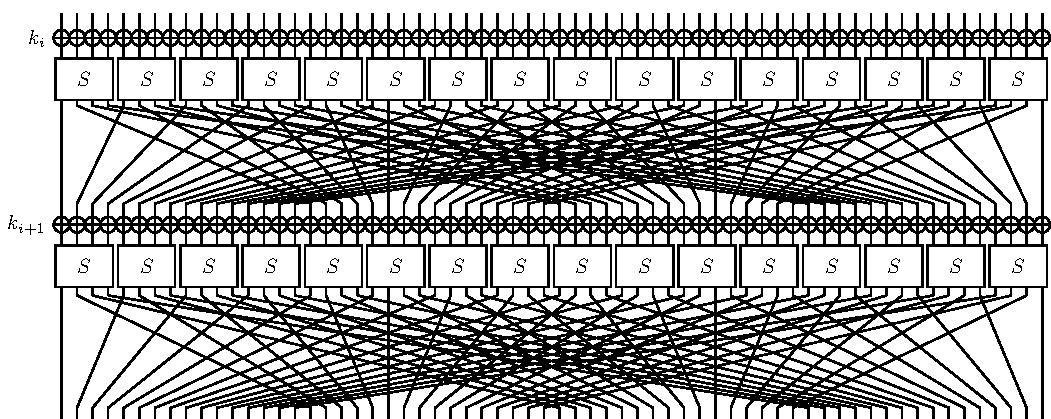
\includegraphics[width=0.7\linewidth]{Images/sa_cipher}
  	\caption{
  		{\footnotesize دور 
  		$i$ 
  		ام از یک 
  		\lr{XSL-Cipher}
  		که لایه‌ی خطّی آن فقط شامل یک جایگشت است}}
  	\label{fig:BlockCipher2}
\end{figure}
  
      به طور خلاصه در یک رمز قالبی 
      \lr{XSL}،
      لایه‌های 
      \lr{s-box}
      به‌وسیله‌ی لایه‌های خطی وابسته به کلید به هم متصل می‌شوند و یک شبکه‌ی 
      $N_{r}$
      دوری که در هر دور 
      $b$
      عدد 
      \lr{s-box}
      موازی شده‌اند را تشکیل می‌دهند. به عنوان نمونه‌ای از این نوع رمزها می‌توان به الگوریتم رایندال
      \LTRfootnote{Rijndael}
 اشاره کرد. 
  
 با وجود این‌که حمله‌ی 
  \lr{XSL}
  برای سامانه‌های رمزنگاری 
  \lr{XSL}
  شرح داده شده امّا این حملات به سایر رمز‌های جانشینی-خطی
 حتی در حالت کلی برای سایر رمزهای قالبی نظیر 
  \lr{DES}
  که نگاشت‌های جانشینی آن‌ها از یک ساختار خاص تبعیّت کند قابل تعمیم است.
  
  
  نمادگذاری‌ها در این‌بخش به‌صورت زیر است. 
  
  
  بیت‌های  کلید را با 
  $k_{ij}$
  که 
  $i = 0...N_{r}$
  و
  $j = 0...(B*s - 1)$
  نمایش می‌دهیم. در کل 
  $N_{r}+1$
  کلید دور، خواهیم داشت که توسط الگوریتم استخراج کلید 
%  \LTRfootnote{key schedule}
  استخراج شده و
  $k_{0}$
  و
  $k_{N_{r}}$
  به ترتیب اوّلین و آخرین‌ آن‌ها می‌باشند. بیت 
  $j$
  ام از ورودی دور 
  $i$
  ام (بعد از اعمال کلید دور قبل) از الگوریتم را با 
  $x_{ij}$
  نمایش می‌دهیم. بیت‌های  ورودی‌ لایه‌ی خطّی دور 
  $i$
  ام را با 
  $y_{ij}$
  نمایش می‌دهیم. به همین ترتیب بیت‌های خروجی دور 
  $i$
  ام (پس از اعمال کلید دور) را با 
  $z_{ij}$
  نمایش می‌دهیم. بنابراین
  $Z_{0} = (z_{0j})_{j = 0}^{Bs - 1}$
  نشان دهنده‌ی متن اصلی و 
  $X_{N_{r}+1} = (x_{(N_{r}+1)j})_{j = 0}^{Bs - 1}$
  نشان دهنده‌ی متن رمز شده ‌است . در حمله‌ای 
  \lr{XSL}
  هدف پیدا کردن کلید مخفی است و فرض را بر این می‌گذاریم که مهاجم یک یا چند زوج  متن اصلی و رمز شده را دارد  و در واقع، حمله از نوع متن اصلی معلوم است. لذا 
  $X_{N_{r}+1}$
  و
  $Z_{0}$
  مجهول نبوده و ثابت هستند. با توجّه به نمادگذاری‌های فوق داریم:
  $$z_{ij} \oplus k_{ij} = x_{i+1 \ j} \ , \ i = 0...N_{r}$$
  این نماد گذاری‌ها برای سامانه‌ی رمزنگاری 
  \lr{CTC}
  که یک نوع رمز 
  \lr{XSL}
  است در شکل 
  \ref{fig:ctcb10}
  نمایش داده شده است. 
  \begin{figure}
\centering
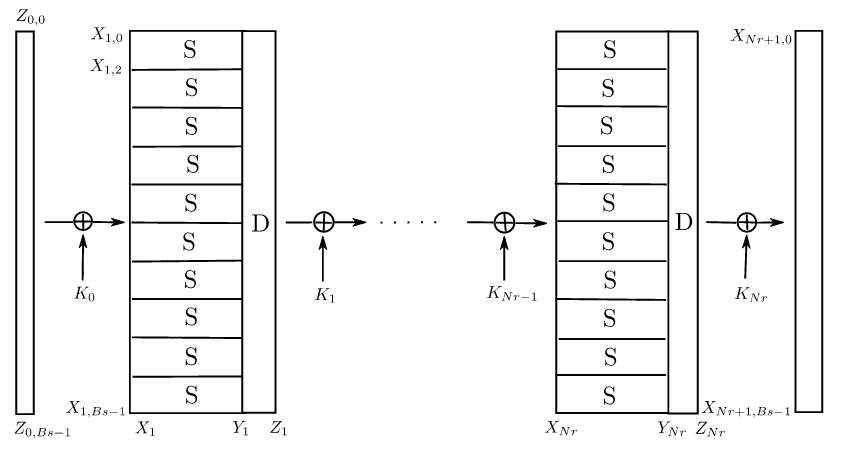
\includegraphics[width=0.85\linewidth]{Images/CTC_10}
\caption{الگوریتم رمزنگاری 
	\lr{CTC}، 
	به ازای 
	$B = 10$}
\label{fig:ctcb10}
\end{figure}

\subsubsection*{سناریوی حمله در روش \lr{XSL}}
 در روش 
 \lr{XSL}
 دو نوع سناریو حمله با نام‌های حمله‌ی عام  (یا نوع اول) و حمله‌ی خاص و(یا نوع دوم) وجود دارد، که در زیر به شرح آن‌ها می‌پردازیم.
 \begin{definition}[\textbf{حمله‌ی 
 		\lr{XSL}
 		عام- صرف نظر از الگوریتم تولید کلید}]
 	در این حمله، هدف یافتن کلید اصلی نیست، بلکه هدف، یافتن کلید هر یک از دور‌ها  است و معادلات بر حسب بیت‌های زیرکلید‌ها (کلید هر یک از دورها)  و سایر متغیرهای میانی سامانه رمزنگاری نوشته می‌شوند. بنابراین مهم نیست که الگوریتم تولید کلید چگونه کار می‌کند.  از آن‌جایی‌که 
 	$N_{r}+1$
 	زیر کلید هم اندازه با متن اصلی وجود دارد به تعداد کافی قید یا معادله نیاز داریم تا این مجهولات را بیابیم از این رو به 
 	$N_{r}+1$
 	زوج متن اصلی و رمز‌شده‌ آن‌ها نیاز داریم. در حالتی که حمله از نوع متن اصلی انتخابی باشد، می‌توان متن‌های اصلی را با این خاصیّت که تنها در تعداد کمی از بیت‌هاي‌ متناظر با یک 
 	\lr{s-box}،
 	متمایز باشند انتخاب کرد تا معادلات به‌دست  آمده برای زوج متن‌های  اصلی و رمز شده دارای مجهولات مشترک بیشتری باشند و تعداد مجهولات کل دستگاه نسبت به حالت عادی کمتر باشد.
 \end{definition}    
 
 \begin{definition}[\textbf{حمله‌ی \lr{XSL} خاص با در نظر گرفتن الگوریتم تولید زیر کلید}]
 	در این سناریو، هدف یافتن کلید مخفی اصلی است. این روش بر این واقعیّت استوار است که الگوریتم‌های تولید کلید در برخی از رمزهای 
 	\lr{XSL}
 	نظیر رایندال و سرپِنت
 	\LTRfootnote{serpent}
 	، 
 	به الگوریتم رمزنگاری متناظرشان شباهت زیادی دارند. لذا در این روش از الگوریتم تولید زیر کلید در حمله‌ی جبری و نوشتن معادلات استفاده می‌شود. بدیهی است که شرط وجود شباهت بین الگوریتم‌های تولید زیر‌کلید و الگوریتم رمزنگاری از عمومیّت این حمله نسبت به حمله‌ی عام می‌کاهد ولی مزیّت آن این است که تنها داشتن یک یا دو زوج متن اصلی -رمزشده برای حمله کفایت می کند.
 \end{definition}

   \subsubsection*{هسته‌ی حمله‌ی \lr{XSL} عام}
   یکی از مراحل اصلی در روش 
   \lr{XSL}
   مرحله‌ موسوم به هسته‌ی 
   \lr{XSL}
   است. هدف این مرحله تولید معادلات مستقل خطی جدید است. این‌کار با ضرب معادلات هر یک از 
   $s-box$
ها در یکجمله‌ای‌هایی که به روشی خاص انتخاب شده‌اند صورت می‌گیرد.
   فرض کنید 
   \textbf{\lr{A}}
   یک 
   \lr{s-box}
   از سامانه‌ی رمز
   \lr{XSL}
   مورد نظر باشد، به 
   \lr{s-box}
   ،
   $A$
   که در این وضعیت آن را انتخاب کرده‌ایم 
   \lr{s-box}
   \textit{فعال}
    و به سایر 
   \lr{s-box}
   ها 
   \lr{s-box}
   های 
   \textit{غیر فعال}
    می‌گوییم. فرض کنید، دستگاه متناظر با 
   $A$ 
   شامل 
   $r$
   معادله‌ی ضمنی درجه‌ی ۲  به‌صورت زیر باشد.
   \begin{equation}
   \label{sboxeq}
   0 = \sum \alpha_{ijk}x_{ij}Y_{ik} + \sum \beta_{ij}x_{ij}+ \sum \gamma_{ij}y_{ij} + \sigma
   \end{equation}
   فرض کنید کنید تعداد یکجمله‌ای‌های موجود در معادله‌ی فوق 
   $t$
   باشد.
   
   فرض کنید 
   $S$
   تعداد کلّ 
   \lr{s-box}
   های شرکت کننده در حمله باشد. از آن‌جایی که در حمله‌ی 
   \lr{XSL}
   عام باید 
   $N_{r}+1$
   زوج متن اصلی-رمزشده متمایز را  در اختیار داشته باشیم  لذا  الگوریتم رمزنگاری باید 
   $N_{r}+1$
   بار اجرا شده باشد. از طرفی در ساختار رمزنگاری از 
   $B\times N_{r}$
   ،
   \lr{s-box}
   استفاده شده است در نتیجه به تعداد 
   $ B\times N_{r}\times (N_{r}+1)$
   دستگاه معادله‌ی مختلف شبیه دستگاه معادله‌ی
   \ref{sboxeq}
   خواهیم داشت و در نتیجه رابطه‌ی 
   $S = B\times N_{r}\times (N_{r}+1)$
   برقرار است.
   
   
   بر خلاف روش 
   \lr{XL}
   که همه‌ی تک جمله‌ای‌ها از درجه‌ی 
   $D-2$
   را در معادلات دستگاه ضرب می‌کردیم این بار این کار  را به صورت گزینشی و نه برای همه‌ی یکجمله‌ای‌ها انجام می‌دهیم. برای این گزینش از پارامتری 
   تحت عنوان 
   \textit{پارامتر بحرانی}
    استفاده می‌کنیم و آن را با 
   $P$
   نمایش می‌دهیم.   
   
   \begin{definition}[\textbf{پارامتر بحرانی}]
   پارامتر بحرانی 
%   \LTRfootnote{critical parameter}
   ، که آن را با 
   	$P$
   	نمایش می‌دهیم، نشان دهنده‌ این است که، برای به‌دست  آوردن معادلات جدید برای یک 
   	\lr{s-box}
   	فعال، باید تمام معادلات آن‌را در تمام یکجمله‌ای‌های حاصل از  ضرب 
   	$p-1$
   	یکجمله‌ای انتخاب شده از  
\lr{s-box}
های غیرفعال،  ضرب کنیم. برای مثال اگر 
   	$P = 2$
   	، آن‌گاه به منظور اضافه کردن معادلات جدید به دستگاه معادلات متناظر با یک
   	\lr{s-box}
   	فعّال، معادلات آن‌را در تمام تک جمله‌ای‌های به‌دست  آمده از 
   	\lr{s-box}
   	های غیر فعّال  ضرب می‌کنیم و اگر 
   	$P = 3$
   	باید معادلات 
   	\lr{s-box}
   	فعال را در  تمام یکجمله‌ای‌های حاصل از ضرب دو یکجمله‌ای به‌دست  آمده از دو 
   	\lr{s-box}
   	غیرفعال ضرب کنیم.
   \end{definition}
   
   تعداد کلّ معادلات به‌دست  آمده پس از افزودن معادلات جدید برابر است با:
   $$R \approx r\times S\times t^{P-1}\times \binom{S-1}{P-1}$$
   تعداد همه‌ی یکجمله‌ای‌های ظاهر شده در معادلات جدید که با 
   $T$،
   نمایش می‌دهیم در زیر محاسبه شده. 
   $$T\approx \frac{R}{r}*t = t^{p}\times S\times \binom{S-1}{P-1} = t^{p}\times P\times\binom{S}{P} \approx t^{p}\times \binom{S}{P}$$
   معادلات جدید که در گام هسته‌ی 
   \lr{XSL}
   و با ضرب یکجمله‌ای‌ها در معادلات دستگاه به‌دست  می‌آیند دارای وابستگی خطی بوده و اعمال روش خطی‌سازی روی آن‌ها کارایی ندارد. به همین دلیل قبل از عملیات خطی سازی با استفاده از روشی موسوم به روش 
   $T'$
   تعداد معادلات مستقل خطی را افزایش می‌دهیم.
   
   پس از حذف معادلات وابسته‌ی خطی، تعداد کلّ معادلات و یکجمله‌ای‌ها به صورت زیر خواهد بود:
   $$R\approx \binom{S}{P}(t^{P}-(t-r)^{P})$$
   $$T\approx \binom{S}{P}(t-r)^{P}$$

 
\subsubsection*{روش 
	$T'$}
 در حمله‌ی 
\lr{XSL}
، مرحله‌ای وجود دارد که بدون تولید یکجمله‌ای‌های جدید، تعداد معادلات مستقل را افزایش می‌دهد. این مرحله به 
روش 
$T'$
%\LTRfootnote{$T'$-Methode}
معروف است. روش 
$T'$،
آخرین مرحله قبل از خطی‌سازی در حمله‌ی 
\lr{XSL}
را تشکیل می‌دهد. به‌یاد داریم که عملیات خطی‌سازی زمانی در حل دستگاه مؤفق عمل می‌کند که تعداد معادلات مستقل خطی، تقریباً برابر با تعداد یکجمله‌ای‌های دستگاه باشد. معمولاً دستگاه به‌دست  آمده از مرحله‌ هسته‌ 
\lr{XSL}، 
 به اندازه‌ی کافی معادله‌ی مستقل ندارد. هدف 
روش 
$T'$
این است که کمبود معادلات مستقل را بدون این‌که یکجمله‌ای جدیدی به دستگاه اضافه شود جبران کند. به این ترتیب دستگاه‌ی که از مرحله‌ی 
$T'$
عبور کرده و به مرحله‌ی نهایی خطی‌سازی می‌رسد، به اندازه‌ی کافی معادله‌ی مستقل خطی خواهد داشت. روش 
$T'$
در 
\cite{courtois2002cryptanalysis}
برای معدلات روی میدان 
$\ffld_{2}$
معرفی شده ولی می‌توان آن را به نحوی مناسب برای میدان‌های دیگر نیز طراحی کرد. 

\begin{definition}[\textbf{$\mT'_{i}$}]
اگر 
$\mT$
مجموعه‌ی  همه‌ی یکجمله‌ای‌های دستگاه باشد، مجموعه‌ی 
$\mT'_{i}$
مجموعه‌ی همه‌ی یکجمله‌ای‌هایی از دستگاه است که به ازای آن‌ها داریم، 
$x_{i}\mT'_{i}\subseteq \mT$.
به عبارت دیگر با ضرب متغیر 
$x_{i}$
در یکجمله‌ای‌های موجود در 
$\mT'_{i}$
، یکجمله‌ای جدیدی به دستگاه اضافه نمی‌شود. در ادامه  اندازه‌ی 
$\mT'$
را با 
$T'$
نمایش می‌دهیم. 
\end{definition}

فرض  کنید 
$\mS\subseteq \ffld_{2}[x_{1},...,x_{n}]$
یک دستگاه معادلات چندجمله‌ای باشد که دارای 
$E$
معادله‌ی مستقل خطی است. در ضمن فرض کنید به ازای هر 
$1\leq i\leq n$
داشته باشیم، 
$E\geq T - T'_{i} + C_{i}$
که 
$C_{i}\geq 1$
یک ثابت است. در این‌صورت الگوریتم روش 
$T'$
به‌صورت زیر تعداد معادلات مستقل خطی دستگاه 
$\mS$
را افزایش می‌دهد. 
\begin{algorithm}[H]
	\renewcommand{\algorithmicrequire}{\textbf{ورودی}}
	\renewcommand{\algorithmicensure}{\textbf{خروجی}}
	\caption{\lr{$T'$-Method}}
	\label{T' method}
	\begin{algorithmic}[1]				
		\REQUIRE دستگاه 
		$\mS:= \{f_{1},...,f_{m}\}\in \polyring$
		با 
	$E$
	معادله‌ی مستقل خطی، بطوری که 
	$E\geq T - T'_{i} + C_{i}$
	و
	$C_{i}\geq 1$.
		\ENSURE 
		دستگاه 
		$\mS'$ 
		با همان یکجمله‌ای‌های موجود در 
		$\mS$
		، و با 
		$E$
		معادله‌ی مستقل خطی بطوری که 
		{\small $E = T - 1$}.
		\STATE دو متغیر 
		$x_{i}$
		و
		$x_{j}$
		را انتخاب کرده و 
		$\mT'_{i}$
		و
		$\mT'_{j}$
		را به‌دست  می‌آوریم. 
		
		\STATE با استفاده از عملیات حذفی گاوس  یکجمله‌ای‌های موجود در 
		$\mT\backslash \mT'_{i}$
		را بر حسب یکجمله‌ای‌های 
		$\mT'_{i}$
		می‌نویسیم. همین کار را برای 
		$\mT'_{j}$
		نیز انجام می‌دهیم. بعد از انجام این‌کار با توجه به شرط 
		$E\geq T - T'_{i} + C_{i}$
		، تقریباً 
		$C_{i}$
		معادله خواهیم داشت که تمام یکجمله‌ای‌های آن متعلق به 
		$\mT'_{i}$
		است. (همین وضعیت برای دستگاه متناظر با 
		$\mT'_{j}$
		نیز برقرار است.)  مجموعه‌ی معادلاتی از دستگاه اول را که فقط بر حسب یکجمله‌ای‌های 
		 $\mT'_{i}$
		 هستند با 
		 $\mC_{i}$
		و مجموعه‌ی معادلاتی از دستگاه دوم، که فقط بر حسب جملات 
		$\mT'_{j}$
است را با 
$\mC_{j}$
نمایش می‌دهیم. 
%3
\STATE معادلات 
$\mC_{i}$
را در 
$x_{i}$
و معادلات 
$\mC_{j}$
را در 
$x_{j}$
ضرب می‌کنیم. بدیهی است که با این‌کار هیچ یکجمله‌ای جدیدی بوجود نمی‌آید. 
\STATE  یکجمله‌ای‌های به‌دست  آمده پس از ضرب 
$x_{i}$
در 
$\mC_{i}$
را بر حسب یکجمله‌ای‌های 
$\mT'_{j}$
و یکجمله‌ای‌های به‌دست  آمده پس از ضرب 
$x_{j}$
در 
$\mC_{j}$
را بر حسب یکجمله‌ای‌های 
$\mT'_{i}$
بازنویسی می‌کنیم. معادلات مستقل خطی به‌دست  آمده را به دستگاه 
$\mS$
اضافه می‌کنیم. 
%4
\STATE 
گام‌های ۱ تا ۴ را تا رسیدن به شرط 
$E = T - 1$
تکرار می‌کنیم. اگر الگوریتم به ازای 
$\mT'_{i}$
و
$\mT'_{j}$
انتخاب شده به شکست انجامید، با دو زوج دیگر مثل 
$\mT'_{k}$
و
$\mT'_{l}$
الگوریتم را از سر می‌گیریم.
	\end{algorithmic}
\end{algorithm}
نویسندگان در 
\cite{courtois2002cryptanalysis}
ادعا کرده‌اند که اگر دستگاه اولیه دارای جواب یکتا باشد، تعداد معادلات مستقل در الگوریتم 
$T'$
به‌صورت نمایی افزایش یافته، بطوری‌که الگوریتم پس از متناهی مرحله اجرا با رسیدن تعداد معادلات مستقل به عدد 
$T - 1$
پایان می‌یابد. 
الگوریتم فوق را با مثالی از ارائه دهندگان این روش در 
\cite{courtois2002cryptanalysis}،
به‌صورت دقیق‌تر شرح می‌دهیم. 
  \begin{example}[\lr{$T'$-Methode}]
  	فرض کنید تعداد متغیّر‌ها 
  	$n = 5$
  	باشد در این صورت 
  	$T = 16$
  	و 
  	$T' = 10$.
  	ما با یک معادله‌ی تصادفی با جواب یکتا، که در آن 
  	$E =  T-T' + 2$
  	 (یعنی  دو معادله‌ی اضافی دارد )، آغاز می‌کنیم. 
  	$\mathcal{T}'_{1}$
  	را متناظر با 
  	$x_{1}$
  	و 
  	$\mathcal{T}'_{2}$
  	را متناظر با متغیّر 
  	$x_{2}$
  	در نظر می‌گیریم. 
  	
  	دستگاه مورد نظر پس از این‌که تمام یکجمله‌ای‌های آن بر حسب یکجمله‌ای‌های 
  	$\mathcal{T}' = \mathcal{T}'_{1}$
نوشته شده‌اند به‌صورت زیر است. 
  {\footnotesize 	\begin{equation}
  	\label{eqsys1}
  	\left \{ \begin{array}{l}
  	x_3 x_2 = x_1 x_3 + x_2\\
  	x_3 x_4 = x_1 x_4 + x_1 x_5 + x_5\\
  	x_3 x_5 = x_1 x_5 + x_4 + 1\\
  	x_2 x_4 = x_1 x_3 + x_1 x_5 + 1\\
  	x_2 x_5 = x_1 x_3 + x_1 x_2 + x_3 + x_4\\
  	x_4 x_5 = x_1 x_2 + x_1 x_5 + x_2 + 1\\
  	0 = x_1 x_3 + x_1 x_4 + x_1 + x_5\\
  	1 = x_1 x_4 + x_1 x_5 + x_1 + x_5
  	\end{array} \right.
  	\end{equation}}
  	به طور مشابه با نوشتن تمام یکجمله‌ای‌های دستگاه اصلی بر حسب یکجمله‌ای‌های 
  	$\mathcal{T}' = \mathcal{T}'_{2}$
  	دستگاه به‌صورت زیر درمی‌آید.  
  {\footnotesize 	\begin{equation}
  	\label{eqsys2}
  	\left \{ \begin{array}{l}
  	x_1 x_3 = x_3 x_2 + x_2\\
  	x_1 x_4 = x_3 x_2 + x_2 + x_1 + x_5\\
  	x_1 x_5 = x_2 x_4 + x_3 x_2 + x_2 + 1\\
  	x_3 x_5 = x_2 x_4 + x_3 x_2 + x_2 + 1 + x_4 + 1\\
  	x_3 x_4 = x_2 x_4 + x_1 + 1\\
  	x_4 x_5 = x_1 x_2 + x_2 x_4 + x_3 x_2\\
  	0 = x_1 x_2 + x_2 x_5 + x_3 x_2 + x_2 + x_3 + x_4\\
  	0 = x_2 x_4
  	\end{array} \right.
  	\end{equation}}
  	توجه کنید که هر دو دستگاه فوق، فقط نمایش‌های متفاوتی از یک دستگاه هستند. در این مرحله، رتبه دستگاه خطّی متناظر، برابر ۸ است.  دو معادله‌ی آخر دستگاه 
  	\ref{eqsys1}
فقط بر حسب یکجمله‌ای‌های موجود در 
$\mT'_{1}$
هستند، بنابراین با ضرب این معادلات در 
  	$x_{1}$
، بدون این که هیچ یکجمله‌ای جدیدی بوجود آید معادلات زیر را به‌دست  می‌آوریم.
  	\begin{equation}
  	\label{eqsys3}
  	\left \{ \begin{array}{l}
  	0 = x_1 x_3 + x_1 x_4 + x_1 + x_1 x_5\\
  	0 = x_{1}x_{4}
  	\end{array} \right.
  	\end{equation}
  	چون معادلات فوق نسبت به معادلات دستگاه اول، مستقل خطی هستند، با اضافه کردن آن‌ها به دستگاه اصلی، رتبه‌ی دستگاه به ۱۰ افزایش پیدا می‌کند.
  	
  	
  	اکنون معادلات به‌دست  آمده در 
  	\ref{eqsys3}
  	را با استفاده از معادلات دستگاه 
  	\ref{eqsys2} 
  	بازنویسی می‌کنیم تا معادلات به‌دست  آمده فقط بر حسب یکجمله‌ای‌های موجود در 
  	$\mathcal{T}'_{2}$
  	باشند. به این ترتیب چهار معادله‌ی اضافی (۲ معادله که از قبل وجود داشت به همراه دومعادله که در این گام به‌دست  آوردیم) برای دستگاه 
  	\ref{eqsys2}
  	به صورت زیر داریم:
  	\begin{equation}
  	\label{eqsys4}
  	\left \{ \begin{array}{l}
  	0 = x_1 x_2 + x_2 x_5 + x_3 x_2 + x_2 + x_3 + x_4\\
  	0 = x_2 x_4\\
  	0 = x_2 x_4 + x_3 x_2 + x_5 + x_2 + 1\\
  	0 = x_3 x_2 + x_2 + x_1 + x_5\\
  	\end{array} \right.
  	\end{equation}
  	بدون این که هیچ یکجمله‌ای جدیدی بوجود آید معادلات دستگاه
  	\ref{eqsys4}
  	را در 
  	$x_{2}$
  	ضرب می‌کنیم و به معادلات زیر می‌رسیم:
  	\begin{equation}
  	\label{eqsys5}
  	\left \{ \begin{array}{l}
  	0 = x_1 x_2 + x_2 x_5 + x_2 x_4 + x_2\\
  	0 = x_2 x_4\\
  	0 = x_2 x_4 + x_3 x_2 + x_5 x_2\\
  	0 = x_3 x_2 + x_2 + x_1 x_2 + x_2 x_5\\
  	\end{array} \right.
  	\end{equation}
  	در مورد معادله‌ی دوّم خوش‌شانس نبودیم چرا که تحت ضرب در 
  	$x_{2}$
  	ناورداست و شکل آن تغییری نمی‌کند با این حال تا این مرحله مؤفق شده‌ابم که سه معادله‌ی مستقل خطی جدید دیگر به‌دست  آوریم. به این ترتیب رتبه دستگاه به عدد ۱۳ می‌رسد. معادلات مستقل جدید را به دستگاه اضافه می‌کنیم. 


  	سه معادله‌ی جدید به‌دست  آمده از مرحله‌ی قبل را با استفاده از دستگاه 
  	\ref{eqsys1}
  	بازنویسی می‌کنیم تا تمام جملات معادلات بر حسب یکجمله‌ای‌های موجود در 
  	$\mathcal{T}'_{1}$
  	باشد. به این ترتیب به معادلات زیر می‌رسیم:
  	\begin{equation}
  	\label{eqsys6}
  	\left \{ \begin{array}{l}
  	1 = x_1 x_5 + x_2 + x_3 + x_4\\
  	1 = x_1 x_2 + x_1 x_3 + x_1 x_5 + x_2 + x_3 + x_4\\
  	0 = x_3 + x_4
  	\end{array} \right.
  	\end{equation}
  	معادلات فوق نسبت به  سایر معادلات موجود در دستگاه  مستقل خطی نیستند و رتبه‌ی دستگاه همان ۱۳ باقی‌ می‌ماند.\\
  	بدون این که هیچ یکجمله‌ای جدیدی بوجود آید معادلات فوق را در 
  	$x_{1}$
  	ضرب می‌کنیم و به معادلات زیر می‌رسیم:
  	\begin{equation}
  	\label{eqsys6}
  	\left \{ \begin{array}{l}
  	1 = x_1 x_5 + x_1 x_2 + x_1 x_3 + x_1 x_4\\
  	1 = x_1 x_5 + x_1 x_4\\
  	0 = x_3 + x_4
  	\end{array} \right.
  	\end{equation}
  	عملیات فوق با به‌دست  آوردن یک معادله مستقل خطّی جدید همراه است و به این ترتیب رتبه‌ی دستگاه به عدد 
  	$14$
  	می‌رسد. با استفاده از دستگاه 
  	\ref{eqsys2}
  	معادله‌ی مستقل به‌دست  آمده از مرحله‌ی قبل را بر حسب یکجمله‌ای‌های 
  	$\mathcal{T}'_{2}$
  	می‌نویسم:
  	$$0 = x_1 x_2 + x_2 x_4 + x_3 x_2 + x_1 + x_2 + x_5 $$
  	معادله‌ی فوق نسبت به معادلات دستگاه، معادله‌ی مستقلی نیست، با ضرب آن در 
  	$x_{2}$
  	(بدون این که هیچ یکجمله‌ای جدیدی بوجود آید) معادله‌ی مستقل خطی زیر را به‌دست  می‌آوریم:
  	$$0 = x_2 x_4 + x_3 x_2 + x_2 x_5 + x_2$$
  	در نتیجه با اضافه کردن این معادله به دستگاه اصلی، رتبه‌ی دستگاه به عدد 
  	$\text{\lr{rank}} = 15$
  	می‌رسد!  این بیشنه‌ی رتبه‌ای است که می‌توان برای دستگاه داشت چرا که تعداد یکجمله‌ای‌های غیر صفر موجود در دستگاه (و در نتیجه تعداد متغیّر‌های دستگاه خطّی ) برابر ۱۵ است. 
\end{example}
روش 
$T'$
گرچه برای اولین بار در حمله‌ی 
\lr{XSL}
در 
\cite{courtois2002cryptanalysis}
، معرفی شد، ولی روشن است که می‌توان از آن در روش 
\lr{XL}
نیز استفاده کرد. در ادامه بخش دیگری از الگوریتم 
\lr{XSL}
، که به هسته‌ی الگوریتم معروف است را معرفی می‌کنیم.


\subsubsection*{الگوریتم 	\lr{XSL}}
الگوریتم 
\lr{XSL}
از کنار هم قرار دادن مراحل قبلی، به صورت زیر به‌دست  می‌آید.
\renewcommand{\algorithmicrequire}{\textbf{ورودی}}
\renewcommand{\algorithmicensure}{\textbf{خروجی}}
%\renewcommand{\algorithmicprint}{\textbf{break}}
\begin{algorithm}[H]
	\caption{الگوریتم
		\lr{XSL}}
	\label{ٓXSL alg}
	\begin{algorithmic}[1]				
		\REQUIRE دستگاه معادلات چندجمله‌ای مربعی به‌دست  آمده از سامانه‌ی رمزنگاری 
		\lr{XSL}
		\ENSURE جواب دستگاه 
		\STATE فرض کنید هر 
		\lr{s-box}
		دارای 
		$r$
		معادله و 
		$t$
		یکجمله‌ای باشد. یک پایه‌ی خطی از بین یکجمله‌ای‌ها شامل 
		$t - r$
		یکجمله‌ای انتخاب کرده (به انضمام ۱ و بجز متغیرها) و 
		$r$
		یکجمله‌ای دیگر را بر حسب آن‌ها می‌نویسیم.		
		\STATE پارامتر بحرانی 
		$P$
		را انتخاب می‌کنیم.(راجع به نحوه‌ی انتخاب بهینه‌ی 
		$P$
		در 
		\cite{courtois2002cryptanalysis}
		بحث شده است.) معادلات به‌دست  آمده از لایه‌های خطی را در یکجمله‌ای‌های پایه‌ی 
		$P - 1$
		،
		\lr{s-box}
		مختلف ضرب می‌کنیم. 
		\STATE تا جایی که امکان دارد، همه‌ی یکجمله‌ای‌ها را به‌صورت ترکیب خطی از یکجمله‌ای‌های پایه می‌نویسیم.
		\STATE الگوریتم 
		$T'$
		را روی معادلات به‌دست  آمده از مرحله‌ی قبل اعمال می‌کنیم.
		\STATE خروجی الگوریتم 
		$T'$
		با روش خطی‌سازی به‌راحتی قابل حل است، لذا آن‌را خطی‌سازی کرده و با روش حذفی گاوس حل می‌کنیم.
	\end{algorithmic}
\end{algorithm}
الگوریتم 
\lr{XSL}
 یک الگوریتم عمومی برای حل دستگاه‌های چندجمله‌ای نیست و فقط برای حل دستگاه‌های خاص متناظر با رمزهای قالبی 
 \lr{XSL}
 نظیر 
 \lr{AES}
 و
 \lr{Serpent}
 طراحی شده است. از آنجایی‌که تحلیل‌های صورت گرفته توسط ارائه‌ دهندگان حمله‌ی 
 \lr{XSL}
 در 
 \cite{courtois2002cryptanalysis}
 مورد پذیرش عموم رمزنگارها نیست و بحث‌های زیادی بر سر کارایی این حمله وجود دارد،(برای نمونه بنگرید به 
 \cite{xiao2003applicability, murphy2003comments})
بررسی بیشتر این روش را رها کرده و به مطالعه  روش‌های  جدیدتری که برای بهبود الگوریتم 
\lr{XL}
ارائه شده است، می‌پردازیم. 
\subsection{روش 
	\lr{MutatntXL}}
روش 
\lr{MutantXL}
که به اختصار آن را با نماد 
\lr{MXL}
نمایش می‌دهیم، اولین بار در سال ۲۰۰۸، توسط دینگ
\LTRfootnote{Ding}
 و همکاران در 
\cite{ding2008mutantxl}
به عنوان یکی دیگر از نسخه‌های بهبود یافته‌ی روش 
\lr{XL}، 
معرفی شد. به‌طور کلی بسیاری از روش‌ها نظیر 
\lr{XL}
 و
\lr{F4}
برای حل دستگاه چندجمله‌ای 
\begin{equation*}
	\mS:= \left \{ \begin{array}{l}
f_{1}(x_{1},...,x_{n}) = 0\\
f_{2}(x_{1},...,x_{n}) = 0\\
\ \ \vdots\\
f_{m}(x_{1},...,x_{n}) = 0
\end{array} \right.
\end{equation*}


ابتدا با ضرب یکجمله‌ای‌ها در معادلات دستگاه، اعضای بیشتری از ایده‌ال تولیده شده توسط چندجمله‌ای‌های دستگاه یعنی 
$I = \langle f_{1},...,f_{m}\rangle$،
را می‌یابند. سپس دستگاه جدید را خطی‌سازی، و در انتها با عملیات حذفی گاوس  آن را حل می‌کنند.  ارائه دهندگان
\lr{MXL}
با آزمایش‌هایی روی روش‌های مذکور، مشاهده کردند که طی مرحله‌ی حذفی گاوس، چندجمله‌ای‌هایی که درجه‌ی آن‌ها کمتر از آن چیزی است که در ابتدا به‌نظر می‌رسد، یا به عبارت دیگر چندجمله‌ای‌هایی که درجه‌ی آن‌ها در مرحله‌ی حذفی گاوس کاهش می‌یابد، می‌توانند سبب تسریع در فرآیند الگوریتم شوند. آن‌ها این چندجمله‌ای‌ها را 
\textit{تغییر‌پذیر}
%\LTRfootnote{mutant}
نامیده و از آن‌ها برای بهبود الگوریتم 
\lr{XL}
استفاده کردند. در ادامه این چندجمله‌ای‌ها را به‌صورت دقیق تعریف کرده و الگوریتم 
\lr{MXL}
را معرفی می‌کنیم. 

فرض کنید 
$\ffld_{q}$
یک میدان متناهی از مرتبه‌ی 
$q$
و 
$f_{1},...,f_{m}\in\ffld_{q}[x_{1},...,x_{n}]$
چندجمله‌ای‌های دستگاه باشند. چون هدف ما پیدا کردن جواب‌هایی از دستگاه است که در 
$\ffld_{q}$
هستند، لذا روی حلقه‌ی خارج قسمتی 
$$R:=\frac{\qfpolyring}{\langle x_{1}^{q} - x_{1},...,x_{n}^{q} - x_{n}\rangle}$$
کار می‌کنیم، یا به‌طور معادل هر  چندجمله‌ای از 
$R$
را به پیمانه‌ی ایده‌ال 
$\langle x_{1}^{q} - x_{1},...,x_{n}^{q} - x_{n}\rangle$
تحویل می‌کنیم. فرضیات فوق تا پایان بحث روش 
\lr{MXL}
، برقرار است. 
\begin{definition}[\textbf{سطح یک چندجمله‌ای}]
فرض کنید 
$I = \langle f_{1},...,f_{m} \rangle $،
و 
$g\in I$
، دارای نمایشی به‌صورت 
$g = h_{1}f_{1} +\cdots + h_{m}f_{m}$
باشد.
\textit{سطح}
%\LTRfootnote{level}
 این نمایش  از 
 $g$، 
 را به‌صورت زیر تعریف می‌کنیم.
$$l = \max\{\deg(h_{i}f_{i})| \ i\in\{1,...,m\}, h_{i}\neq 0 \}.$$
در این‌صورت کوچکترین سطح در بین تمام نمایش‌های 
$g = h_{1}f_{1} +\cdots +h_{m}f_{m}$
را سطح 
$g$
نسبت به 
$F = (f_{1},...,f_{m})$
می‌گوییم و با نماد 
$\level_{F}(g)$
، نمایش می‌دهیم. 
\end{definition}

\begin{definition}[\textbf{چندجمله‌ای تغییر پذیر}]
فرض کنید 
$P = \qfpolyring$
و 
$F = (f_{1},...,f_{m})\subseteq P^{m}$.
چندجمله‌ای 
$g\in P$
را نسبت به 
$F$،
\textit{تغییر‌پذیر}
%\LTRfootnote{Mutant}
گوییم، هرگاه 
$\deg(g) < \level_{F}(g)$.

\end{definition}
به‌طور شهودی وقتی 
$g\in P$
نسبت به 
$F = (f_{1},...,f_{m})$
تغییر پذیر است، یعنی در هر نمایش 
$g$،
 به‌صورت 
$g = h_{1}f_{1}+\cdots +h_{m}f_{m}$،
 یک 
$i \in\{1,...,m\}$
وجود دارد به‌طوری که 
$\deg(g) < \deg(h_{i}f_{i})$.
به عبارت دیگر 
$g$
را نمی‌توان به‌صورت ترکیب خطی از 
$t f_{i}$
ها نوشت بطوری که 
$t$
یک یکجمله‌ای باشد و به ازای هر 
$i$،
 داشته باشیم 
$\deg(t f_{i})\leq \deg(g)$.

\subsubsection*{الگوریتم 
	\lr{MXL}}
فرض کنید 
$P = \qfpolyring$
و
$R = \frac{P}{\langle x_{1}^{q} - x_{1},...,x_{n}^{q} - x_{n}\rangle}$
در این‌صورت روش 
\lr{MXL}
برای حل دستگاه معادلات 
$f_{1} = \cdots = f_{m} = 0$
در الگوریتم 
\ref{MXL alg}
بیان شده است. 
\renewcommand{\algorithmicrequire}{\textbf{ورودی}}
\renewcommand{\algorithmicensure}{\textbf{خروجی}}
%\renewcommand{\algorithmicprint}{\textbf{break}}
\begin{algorithm}
\caption{الگوریتم 
		\lr{MXL}}
\label{MXL alg}	
	\begin{algorithmic}[1]				
		\REQUIRE $F = \{f_{1},...,f_{m}\}\in R$		
		\ENSURE جواب دستگاه معادلات 
		$f_{1} = \cdots = f_{m} = 0$ 
		%1
		\STATE $d = e \gets \min\{\deg(f_{i})| \ f_{i}\in F\}, \ \ G\gets F$
		%2
		\STATE $G$
		را با عملیات حذفی گاوس به‌‌شکل سطری پلکانی تحویل یافته تبدیل می‌کنیم.
		%3
		\STATE اگر 
		$G$
		دارای چندجمله‌ای یک‌متغیره بود، معادله یک‌متغیره را حل کرده و مقدار متناظر با آن متغیر را به‌دست می‌آوریم، اگر دستگاه با این کار حل شود، جواب به‌دست  آمده و الگوریتم متوقف می‌شود و در غیر این‌صورت مقدار به‌دست  آمده را در چندجمله‌ای‌های دستگاه(یا $F$)
		 جایگذاری کرده و به گام ۱ بازمی‌گردیم. اگر دستگاه فاقد چندجمله‌ای یک متغیره باشد به گام ۴ می‌رویم. 
		%4
		\STATE $M\gets \{f\in G| \ \deg(f) < e \}$.
		 {\footnotesize (در واقع چندجمله‌ای‌های 
		 $M$
		 نسبت به 
		 $F$
		 تغییرپذیر هستند.)}
		 %5
		 \STATE اگر 
		 $M\neq \emptyset$،
		  همه‌ی اعضای 
		 $g\in M$
		 را در یکجمله‌ای‌های با درجه‌ 
		 $d - \deg(g)$
		 ضرب کرده و نتایج حاصل از ضرب یکجمله‌ای‌ها  را جایگزین چندجمله‌ای‌های قبلی در 
		 $G$
		 می‌کنیم. قرار می‌دهیم 
		 {\small $e = \min\{\deg(g)| \ g\in M\} + 1$}
		 و به گام ۲ بازمی‌گردیم. در غیر این‌صورت اگر 
		 $M = \emptyset$، 
		 به گام ۶ می‌رویم. 
		 %6
		 \STATE همه‌ی چندجمله‌ای‌های 
		 $g\in G$
		 را با چندجمله‌ای‌های 
		 $x_{i}g$
		 که 
		 $i\in \{1,...,n\}$، 
		  جایگزین می‌کنیم، سپس 
		 $d$
		 را یک واحد افزایش داده، قرار می‌دهیم 
		 $e = d$
		 و به‌ گام ۲ بازمی‌گردیم. 
		
	\end{algorithmic}
\end{algorithm}

اگر گام‌های ۴ و ۵ را حذف کنیم همان الگوریتم 
\lr{XL}
به‌دست  می‌آید. در ضمن در گام ۵ وقتی چندجمله‌ای‌های تغییرپذیر 
 $g$
را در یکجمله‌ای‌های از درجه‌ی 
$d - \deg(g)$
ضرب می‌کنیم، درجه‌ی دستگاه افزایش نمی‌یابد. 
\begin{example}
\label{example:XL_eq}
دستگاه معادلات زیر از حلقه‌ی 
$R = \frac{\ffld_{2}[x_{1},...,x_{4}]}{\langle x_{1}^{2} - x_{1},...,x_{4}^{2} - x_{4} \rangle}$
را در نظر بگیرید. 
\begin{equation*}
\left \{ \begin{array}{l}
f_{1} = x_{1}x_{2} + x_{2}x_{3} + x_{2}x_{4} + x_{3}x_{4} + x_{1} + x_{3} + 1 = 0\\
f_{2} = x_{1}x_{2} + x_{1}x_{3} + x_{1}x_{4} + x_{3}x_{4} + x_{2} + x_{3} + 1 = 0\\
f_{3} = x_{1}x_{2} + x_{1}x_{3} + x_{2}x_{3} + x_{3}x_{4} + x_{1} + x_{4} + 1 = 0\\
f_{4} = x_{1}x_{3} + x_{1}x_{4} + x_{2}x_{3} + x_{2}x_{4} + 1 =0\\
\end{array} \right.
\end{equation*}
طی گام‌های زیر، با استفاده از الگوریتم 
\lr{MXL}
و در نظر گرفتن ترتیب الفبایی مدرج، دستگاه را حل می‌کنیم.
\begin{enumerate}
\item
قرار می‌دهیم 
$d = e = 2$
و
$G = F = \{f_{1},...,f_{4}\}$
\item
پس از عملیات حذفی گاوس دستگاه به‌صورت زیر درمی‌آید.
\begin{equation*}
\left \{ \begin{array}{l}
g_{1} = x_{1}x_{2} + x_{2}x_{3} + x_{2}x_{4} + x_{3}x_{4} + x_{1} + x_{3} + 1 = 0\\
g_{2} = x_{1}x_{3} + x_{1}x_{4} + x_{2}x_{3} + x_{2}x_{4} + x_{1}x_{2} = 0\\
g_{3} = x_{1}x_{4} + x_{2}x_{3} + x_{1} + x_{2} + x_{3} + x_{4} = 0\\
g_{4} = x_{1} + x_{2} + 1 = 0\\
\end{array} \right.
\end{equation*}
\item 
قرار می‌دهیم 
$M = \{g_{4}\}$
. همان طور که مشاهده می‌شود درجه‌ی 
$g_{4}$
پس از عملیات حذفی گاوس کاهش یافته و نسبت به 
$F$
تغییر‌پذیر است. 
\item
قرار می‌دهیم 
$G = \{g_{1},g_{2},g_{3},g_{5}, g_{6}, g_{7}\}$
به‌طوری که 
$g_{5} = x_{1}x_{2}, g_{6} = x_{1}x_{3} + x_{2}x_{3} + x_{3}$
و
$g_{7} = x_{1}x_{4} + x_{2}x_{4} + x_{4}$.
 در ضمن قرار می‌دهیم  
 $e = 2$.
\item
پس از عملیات حذفی گاوس روی 
$G$،
 چندجمله‌ای‌های 
 $g_{5}, g_{6}, g_{7}$
 به‌صورت زیر تغییر می‌کنند. 
 $$\tilde{g}_{5} = x_{2}x_{3} + x_{2}x_{4} + x_{3}x_{4} + x_{1} + x_{3} + 1 \ , \ \tilde{g}_{6} = x_{3}x_{4} + x_{1} + x_{3} + x_{4} + 1 \ , \ \tilde{g}_{7} = x_{3} + x_{4} + 1.$$
\item
قرار می‌دهیم 
$M = \{\tilde{g}_{7}\}$.
\item
چون 
$\deg(\tilde{g}_{7}) = 1$
و
$d = 2$
، لذا همه‌  یکجمله‌ای‌ها از درجه‌ی ۱ را در 
$\tilde{g}_{7}$
ضرب کرده و نتایج به‌دست  آمده که عبارتند از 
$$g_{8} = x_{1}x_{3} + x_{1}x_{4} \ , \ g_{9} = x_{2}x_{3} + x_{2}x_{4} + x_{2} \ , \ g_{10} = x_{3}x_{4},$$
را جایگزین 
$\tilde{g}_{7}$
در 
$G$
می‌کنیم. در ضمن قرار می‌دهیم
$e = 2$.
\item
پس از عملیات حذفی گاوس چندجمله‌ای‌های 
$g_{8}$
و
$g_{9}$
به‌ترتیب به‌صورت 
$\tilde{g}_{8} = x_{2} + x_{4}$
و
$\tilde{g}_{9} = x_{4} + 1$
در می‌آیند. 
\item
با حل معادله‌ی تک‌متغیره‌ 
$\tilde{g}_{9} = 0$
مقدار 
$x_{4}$
برابر با ۱ خواهد بود. با جایگذاری 
$x_{4} = 1$
در دستگاه گسترش پیدا کرده تا کنون، جواب برابر با 
$(x_{1},x_{2},x_{3},x_{4}) = (0,1,0,1)$، 
به‌دست می‌آید. 
\end{enumerate}
ارئه دهندگان 
\lr{MXL}
، اندکی پس از انتشار نسخه‌ی اولیه‌ی این الگورریتم، نسخه‌ی بهبود یافته‌ آن را نیز در  
\cite{mohamed2008mxl2}
، منتشر کردند و آن‌را 
\lr{MXL2}
نامیدند. آن‌ها با استفاده از شبیه‌سازی‌ها به مقایسه‌  الگوریتم 
\lr{MXL2}
با الگوریتم‌ 
\lr{F4}
که یک روش مبنی بر پایه‌ی گروبنر است پرداختند و نشان دادند که ابعاد ماتریس‌های به‌دست  آمده در روش 
\lr{MXL2}
نسبت به 
\lr{F4}
کوچکتر است. آن‌ها همچنین یکسال بعد از انتشار نسخه‌  اولیه‌، در 
\cite{mohamed2009mxl3}
روشی جدید بر پایه‌ی ایده‌ی چندجمله‌ای‌های تغییرپذیر و الگوریتم 
\lr{XL}، 
 برای یافتن پایه‌  گروبنر ایده‌ال‌های صفربعدی، ارائه دادند و آن‌را 
\lr{MXL3}
نامیدند. آن‌ها با انجام آزمایش‌هایی نشان دادند که 
\lr{MXL3}
نه‌ تنها حافظه‌  کمتری در مقایسه با  
\lr{F4}
مصرف می‌کند، بلکه سریع‌تر نیز است.
\end{example}
الگوریتم 
\en{MXL}
در نرم‌افزار 
\en{ApCoCoA}
\cite{ApCoCoA}
 پیاده‌سازی شده، و با دستور 
 \texttt{CharP.MXLSolve(.)}
قابل فراخوانی است. پس از آزمودن این حل‌کننده برای حل دستگاه‌های به‌دست آمده از رمزهای قالبی 
\en{CTC}
و 
\en{SR}
و  رمز دنباله‌ای 
\en{Bivium}، 
مشاهده شد که  این الگوریتم از نظر سرعت تفاوت چندانی با الگوریتم 
\en{XL}
ندارد.  برای مثال سرعت این دو حل‌کننده در جدول 
\ref{tab:comparison_between_XL_and_MXL}، 
به‌ازای دو دستگاه متفاوت مقایسه شده است. محاسبات در رایانه با پردازنده 
$1.6GHz$
و حافظه رم 
$6GB$
و با استفاده از نرم‌افزار 
\en{ApCoCoA}
انجام شده، زمان‌ها بر حسب ثانیه است و 
$m$
و 
$n$
به‌ترتیب نشان‌دهنده تعداد معادلات و تعداد مجهولات هستند. 
\begin{table}
\begin{center}
\begin{tabular}{||c||c|c|c|c|c||}
	\hline 
	& $m$ & $n$ & \en{XL} & \en{MXL}&
	{\footnotesize تعداد جواب‌ها} \\ 
	\hline 
	\hline
	دستگاه مثال
	\ref{example:XL_eq}
	 & $4$ & $4$ & $0.20$ & $0.23$ &
	 $1$\\ 
	\hline 
	{\footnotesize $ CTC(B = 1, N = 1)$} & $26$ & $15$ & $10.84$ & $10.81$ &
	$1$\\ 
	\hline 
\end{tabular} 
\end{center} 
	\caption{مقایسه الگوریتم‌های 
	\en{XL}
و 
\en{MXL}
پیاده‌سازی شده در نرم‌افزار 
\en{ApCoCoA}}
	\label{tab:comparison_between_XL_and_MXL}
\end{table}
 



\section{حمله‌  پایه‌ی گروبنر}
پایه‌های گروبنر کاربردهای زیادی دارد که یکی از مهمترین آن‌ها مسئله‌ی عضویت در ایده‌ال است. می‌دانیم که اگر 
$I$
یک ایده‌ال در 
$P = \polyring$
و 
$G$
یک پایه‌  گروبنر آن‌ باشد، چندجمله‌ای‌ 
$f$
در 
$I$
قرار دارد اگر و تنها اگر
$NF_{G}(f) = 0$.
بنابراین الگوریتمی برای بررسی عضویت یک چندجمله‌ای در یک ایده‌ال وجود دارد. 

کاربرد دیگری که می‌توان به آن اشاره کرد، مسئله‌ی مقایسه‌ی دو ایده‌ال است. اگر 
$I$
و
$J$
دو ایده‌ال در 
$P$
باشند، با محاسبه‌  پایه‌  گروبنر تحویل‌یافته‌  آن‌ها که منحصر بفرد است، می‌توان شمول هر کدام در دیگری و یا تساوی آن‌ها را فقط با مقایسه‌ی پایه‌های آن‌ها دریافت.
امّا کاربردی دیگر که برای ما بیشتر اهمیت دارد حل دستگاه معادلات چندجمله‌ای با استفاده از پایه‌  گروبنر است که در این بخش به آن می‌پردازیم.

%فرض کنید 
%$f_{1},...,f_{m}$
%چندجمله‌ای‌هایی از حلقه‌ی 
%$\fpolyring$
%باشند که 
%$\fld$
%لزماً به طور جبری بسته نیست. دستگاه معادلات زیر را در نظر بگیرید:
%\begin{align*}
%\mS = \left\{
%\begin{array}{lr}
%f_{1}(x_{1},...,x_{n}) = 0\\
%\ \ \ \ \ \ \ \ \  \ \vdots\\
%f_{m}(x_{1},...,x_{n}) = 0	
%\end{array}\right.
%\end{align*}
%ابتدا تعریف دقیقی از مسئله‌ی حل دستگاه فوق ارائه می‌کنیم. 
\begin{definition}[\textbf{فضای آفین}]
	فرض کنید 
	$\ffld$
	یک میدان و 
	$n$
	یک عدد طبیعی باشد. 
	\textit{فضای آفین}
	$n$
	بعدی روی 
	$\ffld$
	عبارت است از مجموعه‌ی زیر،
	$$\ffld^{n}:= \{(a_{1},...,a_{n}) \ : \ a_{1},...,a_{n}\in\ffld\}.$$
\end{definition}
فرض کنید 
$\fld$
یک توسیع جبری میدان 
$\ffld$
باشد. هر چندجمله‌ای مثل 
$f\in\fpolyring$
را می‌توانیم به عنوان تابعی به‌صورت
$$f:\fld^{n}\rightarrow \fld$$
در نظر بگیریم که مقدار این تابع در هر نقطه‌ی 
$(a_{1},...,a_{n})\in \fld^{n}$
با جایگذاری 
$a_{i}$
ها به‌جای 
$x_{i}$
ها در 
$f$
محاسبه می‌شود. چون 
$\fld$
یک توسیع 
$\ffld$
و ضرایب چندجمله‌ای 
$f$
در 
$\ffld\subseteq \fld$
قرار دارند مقدار تابع در 
$\fld$
خواهد بود. منظور از صفر‌های 
$f$
در 
$\fld$
مقادیری است که به ازای آن‌ها تابع 
$f:\fld^{n}\rightarrow\fld$
صفر می‌شود. بنابراین یک چندجمله‌ای مثل 
$f\in\fpolyring$
رفتاری دوگانه دارد، هم می‌تواند به عنوان یک چندجمله‌ای صوری از حلقه‌ی 
$P$
باشد، هم می‌توان آن را به‌صورت یک تابع در نظر گرفت. اما وقتی می‌گوییم 
$f = 0$
است، باید روشن کنیم که 
$f$
به عنوان یک چندجمله‌ای صفر است یا یک تابع صفر است، چرا که این دو می‌توانند متفاوت باشند. برای مثال چندجمله‌ای ناصفر 
$f = x^{2} - x\in \ffld_{2}[x]$
چون به ازای هر مقدار 
$a\in\ffld_{2}$
صفر می‌شود، یک تابع صفر است. بنابراین 
$f$
چندجمله‌ای ناصفری است که متناظر با یک تابع صفر روی فضای آفین 
$\ffld_{2}^{1}$
است. چنین تفاوتی در تعبیر 
$f = 0$
در رمزنگاری که با میدان‌های متناهی کار می‌کنیم امری طبیعی است، ولی وقتی میدان ضرایب چند‌جمله‌ای نامتناهی باشد، ثابت می‌شود
{\small \cite[ص.۳]{IVAcox}}
که 
$f$
به عنوان یک چندجمله‌ای صفر است اگر و تنها اگر به عنوان یک تابع، صفر باشد. 
با این حال می‌دانیم هیچ میدان متناهی نمی‌تواند بسته‌ی جبری باشد.
\begin{definition}[\textbf{واریته یا چندگونای آفین}]
	فرض کنید 
	$\fld$
	یک توسیع از میدان 
	$\ffld$
	و 
	$f_{1},...,f_{m}$
	چندجمله‌ای‌هایی از حلقه‌ی 
	$\fpolyring$
	باشند. مجموعه‌ی 
	$$\mZ(f_{1},...,f_{m}):= \{(a_{1},...,a_{n})\in\fld^{n} \ | \ \fa 0\leq i\leq m  \ f_{i}(a_{1},...,a_{n}) = 0 \}$$
	را 
	$\ffld$-
	\textit{واریته‌ی آفین}
	تعریف شده به‌وسیله‌ 
	$f_{1},...,f_{m}$
	می‌گوییم.
\end{definition}
توجه شود که 
$\ffld$
در عبارت
«$\ffld$-
واریته‌ی آفین» مجموعه‌ی ضرایب چندجمله‌ای را مشخص می‌کند، در حالی که صفرها یا جواب‌ها در 
$\fld^{n}$
قرار دارند. در ادامه برای اختصار 
$\ffld$
-واریته‌ی آفین را واریته‌ی آفین می‌گوییم.
\begin{definition}[\textbf{مسئله‌ی حل دستگاه معادلات چندجمله‌ای}]
	به ازای یک مجموعه‌ی متناهی داده شده مثل 
	$F = \{f_{1},...,f_{m}\}$
	از چندجمله‌ای‌های حلقه‌ی 
	$\fpolyring$،
	مسئله‌ی 
	\textit{حل دستگاه معادلات چندجمله‌ای }
	عبارت است از یافتن واریته‌ی آفین 
	$F$
	یعنی 
	$\mZ (f_{1},...,f_{m})$.
\end{definition}

\begin{lemma}
	فرض کنید 
	$F = \{f_{1},...,f_{s}\}$
	و
	$G = \{g_{1},...,g_{t}\}$
	پایه‌‌های مشترک یک ایده‌ال از حلقه‌ی 
	$\fpolyring$
	باشند. در این‌صورت،
	$$\mZ(f_{1},...,f_{s}) = \mZ(g_{1},...,g_{t}).$$
\end{lemma}
\begin{proof}
	می‌دانیم که 
	$\langle f_{1},...,f_{s}\rangle = \langle g_{1},...,g_{t}\rangle$
	بنابراین اگر 
	$f\in\langle f_{1},...,f_{s}\rangle$
	آن‌گاه 
	$f\in\langle g_{1},...,g_{t}\rangle$
	و در نتیجه چندجمله‌ای‌های 
	$h_{1},...,h_{s}$
	از 
	$P = \fpolyring$
	موجودند بطوری که:
	$$f = h_{1}g_{1} + \cdots + h_{t}g_{t}.$$
	بنابراین به ازای هر 
	$a\in \mZ(g_{1},...,g_{t})$
	داریم،
	$f(a) = 0$.
	چون
	$f$
	را دلخواه انتخاب کردیم، نتیجه می‌شود 
	$a\in \mZ(f_{1},...,f_{s})$
	و
	$\mZ(g_{1},...,g_{t})\subseteq \mZ(f_{1},...,f_{s})$.
	شمول در جهت عکس  را می‌توان بطور مشابه ثابت کرد.
\end{proof}

\begin{definition}
	فرض کنید 
	$I$
	یک ایده‌ال از حلقه‌ 
	$\fpolyring$
	باشد، واریته‌ی آفین تعریف شده به‌وسیله‌ 
	$I$
	عبارت است از
	$$\mZ(I):=\{(a_{1},...,a_{n})\in\fld^{n} \ | \ \fa \ f\in I: \  f(a_{1},...,a_{n}) = 0\}.$$
	که 
	$\fld$
	یک توسیع جبری
	$\ffld$
	است.
\end{definition}

بر اساس قضیه‌  پایه‌  هیلبرت
\ref{hilbert basis th}،
 واریته‌  آفین متناظر با یک ایده‌ال همان واریته‌ی آفین متناظر با مجموعه‌  مولد آن است. 

\begin{theorem}
	اگر 
	$I$
	یک ایده‌ال حلقه‌ 
	$\fpolyring$
	و 
	$F = \langle f_{1},...,f_{m}\rangle$
	یک مولد داده شده برای آن باشد، آن‌گاه، 
	$\mZ(I) = \mZ(f_{1},...,f_{m})$.
\end{theorem}
\begin{proof}
	نتیجه‌ی مستقیم قضیه‌ی پایه‌ی هیلبرت 
	\ref{hilbert basis th}.
\end{proof}
اکنون به دستگاه 
\begin{align*}
\mS = \left\{
\begin{array}{lr}
f_{1}(x_{1},...,x_{n}) = 0\\
\ \ \ \ \ \ \ \ \  \ \vdots\\
f_{m}(x_{1},...,x_{n}) = 0	
\end{array}\right.
\end{align*}
باز می‌گردیم.  نخستین سؤالی که در رابطه با حل دستگاه معادلات به ذهن می‌رسد، مسئله‌  وجود جواب است. پاسخ این سؤال در حالت کلّی داده نشده ولی در حالتی که میدان 
$\fld$
به طور جبری بسته باشد، قضیه‌  صفرهای هیلبرت جواب کاملی ارائه می‌دهد. 
فرض کنید 
$I = \langle f_{1},...,f_{m}\rangle$
در این‌صورت مجموعه‌  جواب دستگاه 
$\mS$
عبارت است از 
$\mZ(I)$.

\begin{theorem}[\textbf{صورت ضعیف قضیه‌ی صفرهای هیلبرت}]
	فرض کنید 
	$\fld$
	یک میدان بطور جبری بسته و
	$I$
	یک ایده‌ال حلقه‌ی 
	$\polyring$
	باشد. در این‌صورت 
	$\mZ(I)$
	تهی است اگر و تنها اگر 
	$I\subsetneqq \fld$.
	یا بطور معادل:
	$$\mZ(I) = \emptyset \  \iff \ 1\in I \ \iff \ I = \polyring$$
\end{theorem}
\begin{proof}
	رجوع کنید به 
	\cite[ص.۱۷۷]{IVAcox}.
\end{proof}
بنابراین، اگر دستگاه 
$\mS$
داده شده باشد، می‌توان با محاسبه‌  پایه‌  گروبنر تحویل‌یافته‌  ایده‌ال تولید شده توسط چندجمله‌ای‌های دستگاه و بررسی این که این پایه برابر 
$\{1\}$
است یا نه، به وجود  یا عدم وجود جواب  برای دستگاه پی‌برد. لازم به ذکر است که وقتی معادلات به‌صورت قطعی   از یک سامانه‌  رمزنگاری به‌دست  آمده‌ باشند دستگاه حتماً جواب خواهد داشت، چون حداقل کلید سامانه و متن اصلی و رمزشده با آن کلید در دستگاه صدق می‌کنند، مگر این‌که در استخراج معادلات سامانه اشتباهی صورت گرفته باشد. 

فرض کنید وجود جواب دستگاه 
$\mS$
برای ما محرز شده باشد، اکنون این سؤال پیش می‌آید که آیا مجموعه‌ی جواب‌های دستگاه یا به عبارتی 
$\mZ(I)$
که 
$I$
ایده‌ال تولید شده توسط معادلات دستگاه است، متناهی است یا نامتناهی؟  یا استفاده از لم تناهی که در ادامه می‌آید، می‌توانیم الگوریتمی برای حل این سؤال ارائه دهیم.


\begin{lemma}[\textbf{محک تناهی}]
	\label{finiteness criterion}
	فرض کنید 
	$\mS$
	دستگاه معادلاتی از چندجمله‌ای‌های 
	$f_{1},...,f_{m}$
	در حلقه‌ی 
	$\fpolyring$
	و 
	$I = \langle f_{1},...,f_{m}\rangle$
	ایده‌ال تولید شده توسط چندجمله‌ای‌های این دستگاه باشد. در ضمن فرض کنید 
	$>$
	یک ترتیب یکجمله‌ای روی 
	$\tn$
	باشد.  در این‌صورت گزاره‌های زیر معادل‌اند:
	\begin{enumerate}
		\item
		دستگاه 
		$\mS$
		دارای تعداد متناهی جواب در 
		$\overline{\ffld}$
		(بستار جبری 
		$\ffld$)
		است.
		\item
		به ازای هر 
		$i = 1,...,n$، 
 داریم  
		$I\cap\ffld[x_{i}]\neq \{0\}$.
		\item
		مجموعه‌ی 
		$\tn\backslash \lm_{>}(I)$
		متناهی است.
		\item
		$\ffld$
		-فضای برداری 
		$\dfrac{\fpolyring}{I}$
		متناهی بعد است.
		\item
		به ازای هر 
		$i\in\{1,...,n\}$
		، عدد 
		$\alpha_{i}\in\mathbb{Z}_{\geq 0}$
		وجود دارد بطوری که 
		$x_{i}^{\alpha_{i}}\in\langle\lt_{>}(I)\rangle$.
	\end{enumerate}
\end{lemma}
\begin{proof}
	رجوع کنید به
	\cite[ص.۲۴۳]{cca1_kreuzer}.
\end{proof}
از بین گزاره‌های معادل در لم
\ref{finiteness criterion}
برقراری گزاره‌های (۳) و (۵) را می‌توان با به‌دست  آوردن پایه‌  گروبنر، برای ایده‌ال 
$I$،
بررسی کرد، در نتیجه مسئله‌  تشخیص متناهی بودن مجموعه‌ی جواب دستگاه 
$\mS$
نیز با استفاده از الگوریتم‌‌های محاسبه‌  پایه‌ی گروبنر، قابل حل است.

\begin{definition}[\textbf{ایده‌ال صفربُعدی}]
	\footnote{وجه تسمیه‌ی صفر بعدی نامیدن اید‌ه‌ال‌هایی که در شرایط لم
		\ref{finiteness criterion}
		صدق می‌کنند، این است که در این ایده‌ال‌ها بعد فضای برداری 
		$\frac{\fpolyring}{I}$
		متناهی است که نتیجه می‌دهد بعد کرول حلقه‌ی 
		$\frac{\fpolyring}{I}$
		باید صفر باشد.}
	ایده‌ال 
	$I = \langle f_{1},...,f_{s}\rangle$
	از حلقه‌ی 
	$P = \fpolyring$
	را 
	\textit{صفر بُعدی}
	گوییم، اگر در یکی از شرط‌های معادل لم 
	\ref{finiteness criterion}
	که یکی از آن‌ها متناهی بودن 
	$\mZ(I)$
	است صدق کند.
\end{definition}


\begin{example}
	فرض کنید
	$P = \mathbb{R}[x,y,z]$
	و ترتیب یکجمله‌ای که به‌کار  می‌بریم ترتیب الفبایی است.  ایده‌ال زیر را در نظر بگیرید،
	$I = \langle x + y + z, xy + xz + yz, xyz - 1 \rangle$
	با استفاده از نرم‌افزار سِیج پایه‌  گروبنر آن را در زیر محاسبه می‌کنیم:
\begin{latin}
\begin{lstlisting}
P.<x,y,z> = PolynomialRing(RR, order = 'lex')
I = sage.rings.ideal.Cyclic(P)
I.groebner_basis()
              [x + y + z, y^2 + y*z + z^2, z^3 - 1.0]
\end{lstlisting}
\end{latin}

%\begin{latin}
%	\begin{sagecommandline}
%		sage: P.<x,y,z> = PolynomialRing(RR, order = 'lex')
%		sage: I = sage.rings.ideal.Cyclic(P)
%		sage: I.groebner_basis()
%	\end{sagecommandline}
%\end{latin}
	
	با توجه به پایه‌  گروبنر به‌دست  آمده مشاهده می‌شود که 
	$\lm(I) = \langle x, y^{2}, z^{3}\rangle$
	و طبق گزاره‌ی (۵) لم
	\ref{finiteness criterion}
	ایده‌ال 
	$I$
	صفربعدی و مجموعه‌  جواب‌های دستگاه متناهی خواهد بود. اگر فرض کنیم 
	$P' = \mathbb{R}[w,x,y,z]$
	آن‌گاه برای ایده‌ال 
	$$J = \langle x + y + z, xy + xz + yz, xyz - 1 \rangle\subseteq P'$$
	به ازای هر 
	$i\in\mathbb{Z}_{\geq0}$
	داریم 
	$w^{i}\notin \langle\lm(J)\rangle$
	و طبق گزاره (۳)
	لم
	\ref{finiteness criterion}،
	$J$
	صفر بعدی نخواهد بود. 
\end{example}
در حالتی که مجموعه‌ی جواب دستگاه چندجمله‌ای
$\mS$
متناهی است علاقه‌مندیم تا تعداد جواب‌ها را بدانیم، قضیه‌ی زیر کرانی برای تعداد جواب‌ها ارائه می‌دهد.
\begin{theorem}
	فرض کنید 
	$f_{1},...,f_{m}\in P = \fpolyring$
	چندجمله‌ای‌های دستگاه معادلات 
	$\mS$
	باشند، اگر 
	$I = \langle f_{1},...,f_{m}\rangle$
	صفربعدی باشد آن‌گاه تعداد جواب‌های دستگاه 
	$\mS$
	در 
	$\bar{F}^{n}$
	حداکثر برابر است با بعد فضای برداری 
	$\frac{P}{I}$.
	به عبارت دیگر داریم
	$$|\mZ(I)|\leq\dim_{\ffld}(\frac{P}{I}).$$
\end{theorem}
\begin{proof}
	رجوع کنید به 
	\cite[ص.۲۴۵]{cca1_kreuzer}
\end{proof}
بنابراین می‌توان در حالت کلّی، کران بالایی برای تعداد جواب‌های یک دستگاه به‌دست  آورد.
\begin{definition}
	رادیکال ایده‌ال 
	$I$
	از حلقه‌ی 
	$P$
	به‌صورت زیر تعریف می‌شود
	$$\sqrt{I}:=\{f\in P \ | \exi m\in\mathbb{N}: f^{m}\in I \}.$$
\end{definition}
به‌راحتی می‌توان نشان داد که 
$\sqrt{I}$
خود یک ایده‌ال است. به ایده‌الی که برابر با رادیکال خودش باشد
\textit{ ایده‌ال رادیکال\textit{}}
می‌گویند.

\begin{definition}[\textbf{میدان کامل}]
	میدان 
	$\ffld$
	یک 
	\textit{میدان کامل}
	است هرگاه، یا مشخصه‌اش صفر باشد و یا اگر دارای مشخصه‌ی ناصفر 
	$p>0$
	است، هر عضو 
	$\ffld$
	دارای ریشه‌ی 
	$p$
	ام باشد.
\end{definition}

برای مثال به ازای هر عدد اوّل 
$p$
میدان
$\ffld_{p}$
یک میدان کامل است چرا که هر عضو آن ریشه‌ی 
$p$
ام خودش است. بطور کلی هر میدان متناهی مثل 
$\ffld_{q}$
که 
$q = p^{e}$
و 
$p$
عددی اوّل است یک میدان کامل است زیرا هر 
$x\in\ffld_{q}$
دارای ریشه‌ی 
$p$
ام 
$x^{p^{e-1}}$
است. در نتیجه همه‌ی میدان‌های متناهی و همچنین همه‌ی میدان‌های نامتناهی که مشخصه صفر دارند میدان‌های کامل هستند.

قضیه‌ی زیر تعداد دقیق جواب‌های دستگاه را وقتی از میدان کامل استفاده می‌کنیم، مشخص می‌کند.

\begin{theorem}
	فرض کنید 
	$I$
	یک ایده‌ال صفر بعدی از حلقه‌ی 
	$P = \fpolyring$
	و
	$\overline{\ffld}$
	بستار جبری 
	$\ffld$
	باشد. در ضمن فرض کنید 
	$\bar{P}:=\bar{\ffld}[x_{1},...,x_{n}]$.
	اگر 
	$\ffld$
	یک میدان کامل باشد آن‌گاه تعداد جواب‌های هر دستگاه معادلات چندجمله‌ای روی
	$\ffld$
	مثل 
	$\mS$
	برابر است با تعداد ایده‌ال‌های ماکزیمال 
	$\overline{P}$
	که شامل ایده‌ال
	$I\overline{P}$
	هستند. در ضمن این عدد دقیقاً برابر است با 
	$\dim_{\ffld}(\frac{P}{I})$.
\end{theorem}
\begin{proof}
	رجوع کنید به 
	{\small \cite[ص.۲۵۳]{IVAcox}}
\end{proof}

در رمزنگاری با میدان‌های متناهی کار می‌کنیم که بسته‌ی جبری نیستند، به همین خاطر به جواب‌هایی که خارج از میدان مورد نظر و  در یک توسیع آن به‌دست  می‌آیند علاقه‌ای نداریم. بنابراین اگر قیدهایی را به دستگاه چندجمله‌ای 
$\mS$
روی میدان 
$\ffld$
اضافه کنیم، به‌طوری‌که به‌واسطه‌  آن‌ها جواب‌ها‌ی دستگاه در 
$\ffld$
محصور شوند، آن‌گاه به هدف خود می‌رسیم. تعریف زیر قیدهای مناسب را به ما معرفی می‌کند.
\begin{definition}[\textbf{چندجمله‌ای‌های میدان}]
	میدان متناهی 
	$\qfpolyring$
	از مرتبه‌ی 
	$q = p^{n}$
	که
	$p$
	یک عدد اوّل و 
	$n$
	یک عدد طبیعی است را در نظر بگیرید. 
	\textit{چندجمله‌ای‌های میدان}
	حلقه‌ی 
	$\qfpolyring$
	عبارتند از
	$$\{x_{1}^{q} - x_{1},...,x_{n}^{q} - x_{n}\}.$$
	در ضمن به ایده‌ال تولید شده توسط مجموعه‌ی فوق یعنی، 
	$$\langle x_{1}^{q} - x_{1},...,x_{n}^{q} - x_{n} \rangle$$
	ایده‌ال میدان 
	$\qfpolyring$
	می‌گوییم. 
\end{definition}

\begin{corollary}
	فرض کنید 
	$\mS$
	یک دستگاه معادلات چندجمله‌ای از حلقه‌ی 
	$\qfpolyring$
	و 
	$I = \langle f_{1},...,f_{m}\rangle$
	ایده‌ال تولید شده توسط چندجمله‌ای‌های دستگاه باشد. در این ‌صورت بعد از اضافه کردن چندجمله‌ای‌های میدان به ایده‌ال
	$I$
	ایده‌ال
	$$I' = \langle f_{1},...,f_{m},x_{1}^{q} - x_{1},...,x_{n}^{q} - x_{n} \rangle$$
	به‌دست  می‌آید که طبق گزاره‌ی (۵) لم 
	\ref{finiteness criterion}
	یک ایده‌ال صفر بعدی است و لذا مجموعه‌ی جواب متناهی خواهد بود.
\end{corollary}

\begin{corollary}
	فرض کنید 
	$I = \langle f_{1},...,f_{m} \rangle$
	یک ایده‌ال از حلقه‌ی 
	$\qfpolyring$
	باشد. اگر 
	$J$
	ایده‌ال تولید توسط
	$$\{f_{1}, ...,f_{m}\}\cup\{x_{1}^{q} - x_{1},...,x_{n}^{q}- x_{n}\}$$
	باشد، آن‌گاه تنها تفاوت واریته‌ی 
	$\mZ(J)$
	با واریته‌ی 
	$\mZ(I)$
	در این است که شامل هیچ‌یک از نقاط 
	$\bar{\ffld}^{n}\backslash \ffld^{n}$
	نیست.
\end{corollary}
\begin{proof}
	در هر میدان متناهی ار مرتبه‌ی 
	$q$
	نظیر 
	$\qffld$
	معادله‌ی 
	$x^{q} = x$
	به ازای هر 
	$x\in \ffld$
	صادق است. بنابراین تمام نقاط 
	$\ffld^{n}$
	در معادلات 
	$x_{i}^{q} - x_{i} = 0$
	به‌ازای 
	$i = 1,...,n$،
	صدق می‌کنند. علاوه بر  این هر یک از چندجمله‌ای‌های 
	$x_{i}^{q} - x_{i}$
	به طور کامل روی 
	$\ffld$
	تجزیه می‌شوند و در نتیجه هیچ‌یک از نقاط 
	$\bar{\ffld}^{n}\backslash \ffld$
	در معادلات 
	$x_{i}^{q} - x_{i}$
	صدق نمی‌کنند. 
\end{proof}

\begin{definition}
	فرض کنید 
	$\mZ\subseteq \ffld^{n}$
	یک 
	$\ffld$-
	واریته‌ی آفین باشد. در این‌صورت 
	$I(\mZ)$
	به‌صورت زیر تعریف می‌شود:
	$$I(\mZ):= \{f\in \fpolyring \ | \ \fa (a_{1},...,a_{n})\in \mZ: \ f(a_{1},...,a_{n}) = 0 \}.$$
\end{definition}

\begin{lemma}
	اگر 
	$\mZ\subseteq \ffld^{n}$
	یک واریته‌ی آفین باشد آن‌گاه 
	$I(\mZ)$
	یک ایده‌ال حلقه‌ی
	$\fpolyring$
	است.
\end{lemma}
\begin{proof}
	به 
	\cite[ص.۳۲]{IVAcox}
	رجوع کنید.
\end{proof}

\begin{theorem}[\textbf{صورت قوی قضیه‌ی صفرهای هیلبرت}]
	فرض کنید 
	$\ffld = \overline{\ffld}$
	و 
	$f_{1},...,f_{s}\in \fpolyring$.
	در این‌صورت،
	$$f\in I(\mZ(\langle f_{1},...,f_{s} \rangle)) \ \iff \ \exi m\in\mathbb{N} : \ f^{m}\in\langle f_{1},...,f_{s}\rangle.$$
	یا به بیان دیگر برای هر ایده‌ال 
	$I\subseteq\fpolyring$
	داریم،
	$I(\mZ(I)) = \sqrt{I}$.
\end{theorem}
\begin{proof}
	به 
	\cite[ص.۱۷۹]{IVAcox}
	رجوع کنید.
\end{proof}



\begin{definition}[\textbf{ایده‌ال حذف}]
	ایده‌ال 
	$I = \langle f_{1},...,f_{s}\rangle\subseteq \fpolyring$
	را در نظر بگیرید. فرض کنید 
	$l\in\{0,..., n-1\}$
	مجموعه‌ی همه‌ی چندجمله‌ای‌هایی از 
	$I$
	که فقط از متغیرهای 
	$x_{l+1},...,x_{n}$
	تشکیل شده‌اند عبارت است از
	$$I_{l} = I\cap\ffld[x_{l+1},...,x_{n}]$$
	که به آن 
	$l$
	امین ایده‌ال حذف 
	$I$
	می‌گوییم.
\end{definition}
با توجه به تعریف ایده‌ال حذف نتیجه می‌شود که 
$I_{l}$
ایده‌الی از حلقه‌ی 
$\ffld[x_{l+1},...,x_{n}]$
است که به آن ایده‌ال حذف 
$I$
نسبت به متغیرهای 
$\{x_{1},...,x_{l}\}$
هم می‌گویند زیرا این ایده‌ال از حذف تمام چندجمله‌ای‌های
$I$
که شامل متغیرهای 
$\{x_{1},...,x_{l}\}$
هستند، به‌دست  می‌آید. 
\begin{proposition}[\textbf{لم سایدنبرگ}]
	\label{seidenberg lemma}	
	فرض کنید 
	$\ffld$
	یک میدان و 
	$P = \fpolyring$
	و
	$I$
	یک ایده‌ال صفر بعدی 
	$P$
	باشد. فرض کنید به ازای هر 
	$i\in\{1,...,n\}$
	چندجمله‌ای ناصفر 
	$g_{i}\in I\cap \ffld[x_{i}]$
	وجود داشته باشد بطوری که 
	$\gcd(g_{i},g'_{i}) = 1$
	باشد. (
	$g'_{i}$
	مشتق 
	$g_{i}$
	نسبت به 
	$x_{i}$
	است) در این‌صورت 
	$I$
	یک ایده‌ال رادیکال است.
\end{proposition}
\begin{proof}
	به 
	\cite[ص.۲۵۱]{IVAcox}
	مراجعه کنید.
\end{proof}
فرض کنید 
$\ffld_{q}$
یک میدان متناهی باشد که 
$q = p^{n}$
و
$p$
یک عدد اوّل است. فرض کنید 
{\small $I = \langle f_{1},...,f_{m}\in\rangle\subseteq\qfpolyring$}،
در این‌صورت دستگاه 
\begin{align*}
\mS = \left\{
\begin{array}{lr}
f_{1}(x_{1},...,x_{n}) = 0\\
\ \ \ \ \ \ \ \ \  \ \vdots\\
f_{m}(x_{1},...,x_{n}) = 0	
\end{array}\right.
\end{align*}
ممکن است جواب‌هایی خارج از 
$\qffld^{n}$
یعنی جواب‌هایی در 
$\bar{\qffld}^{n}\backslash\ffld$
داشته باشد که 
$\bar{\ffld}$
بستار جبری 
$\ffld$
است. طبق لم سایدنبرگ
\ref{seidenberg lemma}
با ضمیمه کردن معادلات 
$$\{x_{i}^{q} - x_{i}: \ 1\leq i\leq n\}$$
به دستگاه 
$\mS$
، ایده‌ال تولید شده توسط معادلات جدید که آن‌را با 
$J$
نمایش می‌دهیم، یک ایده‌ال رادیکال با واریته‌ی 
$\mZ(J) = \mZ(I)\cap \ffld^{n}$
است. 

اگر
$I$
ایده‌ال تولید شده توسط چندجمله‌ای‌های دستگاه 
$\mS$
باشد، می‌دانیم که این ایده‌ال پایه‌های متفاوتی دارد، سؤال این است که آیا این ایده‌ال پایه‌ای دارد که با استفاده از آن بتوان به‌راحتی جواب‌های دستگاه معادلات چندجمله‌ای 
$\mS$
را به‌دست  آورد؟  طبق قضیه‌ی زیر پاسخ این سؤال مثبت است.

\begin{theorem}[\textbf{قضیه‌ی حذف}]
	\label{elimination th}	
	فرض کنید 
	$I\subseteq\fpolyring$
	یک ایده‌ال و 
	$G$
	پایه‌ی گروبنر آن نسبت به ترتیب الفبایی و با فرض 
	$x_{1}> x_{2}>\cdot>x_{n}$
	باشد. در این‌صورت به ازای هر 
	$0\leq l < n$
	، مجموعه‌ی 
	$$G_{l} = G\cap \ffld[x_{l+1},...,x_{n}]$$
	یک پایه‌ی گروبنر برای ایده‌ال 
	$I_{l}$
	است.
\end{theorem}
\begin{proof}
	به 
	\cite[ص.۱۲۳]{IVAcox}
	رجوع کنید.
\end{proof}

\begin{corollary}
	طبق قضیه‌ی حذف پایه‌ی گروبنر یک شکل مثلثی دارد، به این معنی اگر در یک‌جهت مناسب اعضای پایه را انتخاب کنیم هر بار یکی از تعداد متغیرهای ظاهر شده کم می‌شود. برای روشن شدن موضوع به‌یاد بیاورید که برای حل دستگاه معادلات خطّی به روش حذفی گاوس، ابتدا آن را به‌صورت مثلثی تبدیل می‌کردیم و سپس از آخرین معادله که فقط شامل یک مجهول بود شروع به حل می‌کردیم و با به‌دست  آوردن جواب مجهول مورد نظر و جایگذاری آن در معادله‌ی قبلی مجهولات دیگر را پیدا می‌کردیم. مثال بعدی این مطلب را بهتر نشان می‌دهد.
\end{corollary}

\begin{remark}
	همان طور که قبلاً ذکر شد، با استفاده از ترتیب الفبایی است که پایه‌  گروبنر  ایده‌ال، شکل مثلثی به خود می‌گیرد و  امکان استخراج جواب‌های دستگاه فراهم می‌شود. از طرفی می‌دانیم که محاسبه پایه‌  گروبنر با استفاده از ترتیب الفبایی مدرج معکوس سریع‌تر صورت می‌گیرد. بنابراین روش بهینه این است که ابتدا پایه‌  گروبنر را با ترتیب الفبایی مدرج معکوس محاسبه کنیم، سپس با استفاده از الگوریتم‌های تبدیل پایه‌ی گروبنر تحت یک ترتیب به پایه‌ی گروبنر تحت ترتیب دیگر نظیر 
	\cite{faugere1993efficient}
	\lr{FGLM}،
	پایه‌  گروبنر تحت ترتیب الفبایی را به‌دست  آوریم.
\end{remark}
\begin{example}[\textbf{مثلثی سازی دستگاه چندجمله‌ای با پایه‌ی گروبنر}]
	فرض کنید 
	$P = \ffld_{127}[x,y,z]$
	و ترتیب یکجمله‌ای الفبایی را بکار ببریم. ایده‌ال زیر را در نظر بگیرید:
	$$I = \langle x + y + z, xy + xz + yz, xyz - 1 \rangle.$$
	ابتدا معادلات میدان 
	$\ffld_{127}$
	را به آن اضافه کرده، سپس پایه‌ی گروبنر تحویل‌یافته‌ی  آن را محاسبه می‌کنیم.
\begin{latin}
\begin{flushleft}
\begin{lstlisting}
P.<x,y,z> = PolynomialRing(GF(127), order = 'lex')
I = sage.rings.ideal.Cyclic(P); print I
 Ideal (x + y + z, x*y + x*z + y*z, x*y*z - 1) of Multivariate Polynomial
Ring in x, y, z over Finite Field of size 127
J = I + sage.rings.ideal.FieldIdeal(P)
g1, g2, g3 = J.groebner_basis()
g1, g2, g3
                (x + y + z, y^2 + y*z + z^2, z^3 - 1)
\end{lstlisting}
\end{flushleft}
\end{latin}	

%\begin{latin}
%\begin{sagecommandline}
%	sage: P.<x,y,z> = PolynomialRing(GF(127), order = 'lex')
%	sage: I = sage.rings.ideal.Cyclic(P)
%\end{sagecommandline}
%\renewcommand{\sagecommandlinetextoutput}{True}	
%\begin{sagecommandline}
%	sage: I
%\end{sagecommandline}
%\renewcommand{\sagecommandlinetextoutput}{False}	
%\begin{sagecommandline}
%	sage: J = I + sage.rings.ideal.FieldIdeal(P)
%	sage: g1, g2, g3 = J.groebner_basis()
%	sage: g1, g2, g3
%\end{sagecommandline}
%\end{latin}
همان طور که بر اساس قضیه‌  حذف	
\ref{elimination th}
پیش‌بینی می‌کردیم،  و در زیر مشاهده می‌شود،  پایه گروبنر نسبت به ترتیب الفبایی  شکل مثلثی دارد.
\begin{equation*}
\left.
\begin{array}{ll}
&\left.
\begin{array}{ll}
&\{z^{3} + 126,\qquad\bigr\}\quad z \text{{\footnotesize فقط بر حسب}}\\
&\,\,y^{2} + y z + z^{2},\\
\end{array}\right\}\quad y, z\text{{\footnotesize فقط بر حسب}}\\
&\qquad x + y + z\}.
\end{array}\right\}\text{{\footnotesize همه‌ی متغیرها}}
\end{equation*}
	
اکنون به استخراج جواب‌ها می‌پردازیم.
\begin{latin}
\begin{lstlisting}
factor(g3)
                   (z - 19) * (z - 1) * (z + 20)
factor(g2(x,y,-108))
                        (y - 1) * (y + 20)
factor(g1(x,-126,-108))
                              x + 20
all(f(-20, 1, 19) == 0 for f in I.gens())
\end{lstlisting}
\end{latin}	
	
%\begin{latin}
%\begin{sagecommandline}
%sage: factor(g3)
%sage: factor(g2(x,y,-108))
%sage: factor(g1(x,-126,-108))
%sage: all(f(-20, 1, 19) == 0 for f in I.gens())
%\end{sagecommandline}
%\end{latin}
	مجموعه‌ی جواب‌ها یا واریته‌ی آفین 
$\mZ(J)$
	با استفاده از تابع 
\verb|variety|
	از کلاس 
\verb|ideal|
	قابل محاسبه است.
\begin{latin}
\begin{lstlisting}
J.variety()
[{y: 19, z: 1, x: 107}, {y: 107, z: 1, x: 19}, {y: 1, z: 19, x: 107},
{y: 107, z: 19, x: 1}, {y: 1, z: 107, x: 19}, {y: 19, z: 107, x: 1}]
\end{lstlisting}
\end{latin}	
%\renewcommand{\sagecommandlinetextoutput}{True}	
%\begin{latin}
%\begin{sagecommandline}
%sage: J.variety()
%\end{sagecommandline}
%\end{latin}
%\renewcommand{\sagecommandlinetextoutput}{False}		
\end{example}
همان‌طور که مشاهده می‌شود، پایه‌  گروبنر ابزار خوبی برای حل دستگاه‌ معادلات چندجمله‌ای است. در رمزنگاری از الگوریتم‌های بهینه‌شده محاسبه‌  پایه‌ی گروبنر  نظیر 
\en{F4}
و
\en{F5}

الگوریتم‌های محاسبه پایه گروبنر به‌خصوص  الگوریتم 
\en{F4}
در نرم‌افزارهای جبری مانند 
\en{Maple}
\cite{Maple}، 
\en{Singular}
\cite{DGPS}
و 
\en{ApCoCoA}
\cite{ApCoCoA}
پیاده‌سازی شده است.  در جدول 
\ref{tab:comparision_time_of_computation_of_GB}، 
مقایسه‌ای بین الگوریتم‌های پیاده‌سازی شده در این‌نرم‌افزارها صورت گرفته است. زمان‌های گزارش شده بر حسب ثانیه و 
$m$
و 
$n$
به‌ترتیب نشان‌دهنده تعداد معادلات و تعداد مجهولات هستند.  دستگاه‌های معادلات به‌دست آمده مربوط به الگوریتم رمزنگاری قالبی 
\en{CTC}
هستند  که  به‌ازای یک زوج متن اصلی و رمزشده معلوم و  با استفاده از نرم‌افزار 
\en{Sage}
\cite{sagemath}
استخراج گشته‌اند.   در ضمن محاسبات روی یک رایانه با پردازنده 
$1.6GHz$
و حافظه رم 
$6GB$
انجام شده است. 

در جدول 
\ref{tab:comparision_time_of_computation_of_GB}
برای محاسبه جواب دستگاه با استفاده از پایه‌گروبنر در نرم‌افزار 
\en{Maple}، 
از کتاب‌خانه 
\en{FGb}
\cite{FGb}
که آن‌را  مبدع الگوریتم‌های 
\en{F4}
و 
\en{F5}
یعنی فوجِر پیاده‌سازی نموده، استفاده شده است. محاسبه پایه گروبنر در 
\en{ApCoCoA}
نیز با استفاده از دستور 
\texttt{GBasis5(.)}
صورت گرفته که بعد از هر بار فراخوانی این‌دستور 
\en{ApCoCoA}
از کتاب‌خانه 
\texttt{CoCoALib-0.9945}
برای محاسبه پایه گروبنر استفاده کرده است. در نرم‌افزار 
\en{Sage}
نیز برای محاسبه پایه گروبنر از 
\en{Singular}
استفاده شده است. 
\begin{table}
\begin{center}
\begin{tabular}{||c||c|c|c|c|c|c||}
	\hline 
	{\small $CTC(B, N)$} & $m$ & $n$ & \en{Sage(Singular)} &  \en{Maple(FGb)}&  \en{ApCoCoA(CoColib)}&
	 {\footnotesize تعداد جوابها} \\ 
	\hline 
	\hline
	$CTC(1, 1)$ & $26$ & $15$ & $0.020$ & $0.031$  & $0.015$  & $1$ \\ 
	\hline 
	$CTC(2, 2)$ & $98$ & $54$ & $0.064$ & $0.078$ & $0.070$  & $1$ \\ 
	\hline 
	$CTC(2, 3)$ & $144$ & $78$ & $0.128$ & $0.266$ & $0.375$ & $1$ \\ 
	\hline 
	$CTC(3, 2)$ & $147$ & $81$ & $0.224$ & $0.343$ & $0.539$  & $1$ \\ 
	\hline 
	$CTC(4, 2)$ & $196$ & $108$ & $0.352$ & $1.69$ & $3.562$ & $1$ \\ 
	\hline 
	$CTC(3, 3)$ & $216$ & $117$ & $0.904$ & $4.64$ & $9.208$  & $1$ \\ 
	\hline 
	$CTC(3, 4)$ & $285$ & $153$ & $4.28$ & $49.73$  & $598.828$  & $1$ \\ 
	\hline 
	$CTC(4, 3)$ & $288$ & $156$ & $2.61$ & $47.89$  & $420.595$  & $1$ \\ 
	\hline 
\end{tabular} 
\end{center} 
	\caption{مقایسه  الگوریتم‌های محاسبه پایه گروبنر در نرم‌افزارهای 
	\en{Maple}، 
\en{Sage}
و 
\en{ApCoCoA}}
	\label{tab:comparision_time_of_computation_of_GB}
\end{table}
همان‌طور که مشاهده می‌شود سرعت محاسبه پایه گروبنر در 
\en{Singular}
بیشتر از 
\en{Maple}
و در 
\en{Maple}
بیشتر از 
\en{ApCoCoA}
است.   نتیجه دیگری که می‌توان گرفت این است که زمان حل دستگاه به‌دست آمده از 
$CTC$
از بین دو پارامتر 
$B$
و 
$N$
به  تغییرات 
$N$
یعنی تعداد  دورها   حساسیت بیشتری نشان داده است،  به‌طوری که زمان حل با استفاده از پایه گروبنر وقتی تعداد دورها  را افزایش می‌دهیم، بیشتر از زمانی است که با ثابت نگاه داشتن تعداد  دورها،  فقط تعداد  جعبه‌های جانشینی را افزایش می‌دهیم. 




%\subsection*{الگوریتم 	
%	\lr{F4}}
%همان‌طور که قبلاً هم اشاره کردیم، یکی از بهترین الگوریتم‌ها برای یافتن پایه‌ی گروبنر یک ایده‌ال الگوریتم 
%\lr{F4}
%، است که توسط فوجر 
%\cite{faugere1999new}،
%طراحی شده. در این بخش روش کار این الگوریتم را شرح خواهیم داد. 
%
%\begin{definition}[\textbf{ماتریس ضرایب چندجمله‌ای‌ها}]
%فرض کنید 
%$P = \polyring$
%و
%$F = (f_{1},...,)\in P^{m}$
%یک 
%$m$
%تایی مرتب از چندجمله‌ای‌های باشد. یک ترتیب یکجمله‌ای روی 
%$\tn$
%در نظر بگیرید و فرض کنید 
%$$v_{F} = (m_{l},...,m_{1})$$
%بردار شامل اعضای 
%$\Supp(F)$
%به‌صورت نزولی باشد. در این‌صورت ماتریس ضرایب 
%$F$
%که با 
%$A_{F}$
%نمایش می‌دهیم به‌صورت زیر تعریف می‌شود.
%$$A[i,j] = a_{ij} \ \iff \ \text{
%	$a_{ij}$
%	ضریب یکجمله‌ای 
%	$m_{j}$
%	از 
%	$f_{i}$
%	باشد.}$$
%در ضمن به بردار 
%$v_{F}$
%، بردار یکجمله‌ای‌های 
%$F$
%، می‌گوییم. 
%\end{definition}
%با توجه به تعریف فوق، 
%$F$
%را به‌راحتی می‌توان از روی سطرهای 
%$A_{F}*v_{F}$
%به‌دست  آورد. 
%\begin{example}
%فرض کنید، 
%\begin{align*}
%f_{1} =& 81 z^{2} + 51 x + 125 z + 38\\
%f_{2} =& 76 xy + 80 y^{2} + 49 xz + 62 yz + 45 z^{2}\\
%f_{3} =& 122 x^{2} + 106 yz + 78 z^{2} + 48 x + 112 y\\
%\end{align*}
%چندجمله‌ای‌هایی از 
%$\ffld_{127}[x,y,z]$
%باشند. با در نظر گرفتن ترتیب 
%\verb|degrevlex|
%داریم.
%
%	\begin{align*}
%	\begin{pmatrix}
%	f_{1}\\
%	f_{2}\\
%	f_{3}\\
%	\end{pmatrix} = 
%	\begin{pmatrix}
%	0&0&0&0&0&81&51&0&125&38\\
%	0&76&80&49&62&45&0&0&0&0\\
%	122&0&0&0&106&78&48&112&0&0\\
%	\end{pmatrix} \ 
%	\times \begin{pmatrix}
%	x^{2}\\
%	xy\\
%	y^{2}\\
%	xz\\
%	yz\\
%	z^{2}\\
%	x\\
%	y\\
%	z\\
%	1\\
%	\end{pmatrix}
%	\end{align*}
%	
%\end{example}
%
%به‌منظور یافتن پایه‌ی تحویل یافته‌ی یک دستگاه چندجمله‌ای خطی، در واقع کافی است تا عملیات حذفی گاوس را روی ماتریس ضرایب آن دستگاه اعمال کنیم. برای مثال دستگاه خطی شامل معادلات 
%$26y + 52z + 62, 54y + 119 z + 55$
%و
%$41x + 91z + 13$
%روی 
%$\ffld_{127}[x,y,z]$
%داریم. 
%$$A = \begin{pmatrix}
%0&26&52&62\\
%0&54&119&55\\
%41&0&91&13\\
%\end{pmatrix}\xrightarrow{\text{عملیات حذفی گاوس}}\begin{pmatrix}
%1&0&0&29\\
%0&1&0&38\\
%0&0&1&75\\
%\end{pmatrix}$$
%که ماتریس تحویل‌یافته متناظر با چند‌جمله‌ای‌های 
%$x+29, y+38$
%و
%$z + 75$
%است. 
%
%دو چندجمله‌ای 
%$f = x^{2} + 22xy - 2y^{2} + 12z^{2} + 22z$
%و 
%$g = 33x^{2} + y^{2} + z^{2} + x + 2z$
%از حلقه‌ی 
%$\ffld_{127}[x,y,z]$
%را در نظر بگیرید. اگر از ترتیب یکجمله‌ای 
%$degrevlex$
%استفاده کنیم،  ماتریس‌ ضرایب 
%$F = (f,g)$
%عبارت است از 
%$$\begin{pmatrix}
%1&2&125&14&0&22\\
%3&0&1&1&1&2\\
%\end{pmatrix}$$
%که فرم تحویل‌یافته‌ی آن عبارت‌است از 
%$$\begin{pmatrix}
%1&0&85&85&85&43\\
%0&1&20&28&21&53\\
%\end{pmatrix}$$
%که متناظر است با چندجمله‌ای‌های 
%\begin{align*}
%f' = x^{2} + 85y^{2} + 85z^{2} + 85x + 43z,
%g' = xy + 20y^{2} + 28z^{2} + 21x + 53 z.
%\end{align*}
%اگر نتیجه‌ی به‌دست آمده در فوق را با باقی‌مانده‌ی تقسیم 
%$f$
%بر 
%$g$
%که برابر است با 
%$r = 2xy + 40y^{2} + 56z^{2} + 42x + 106 z$ 
%، مقایسه  کنیم، متوجه می‌شویم که 
%$r = 2g'$.
%آیا چنین نتیجه‌ای قابل تعمیم است؟ مثال دیگری را در نظر می‌گیریم. فرض کنید
%\begin{align*}
%f = x^{2} - 2xy - 2y^{2} + 14z^{2}\\
%g = x + 2z.
%\end{align*}
%در ابن مثال، می‌توان دید که فرم کاهش یافته‌ی ماتریس ضرایب هیچ تفاوتی با ماتریس اصلی ندارد. علت این اتفاق این است که 
%$x$
%عضو یکجمله‌ای‌های 
%$f$
%نیست. از طرف دیگر  
%$x$
%دو یکجمله‌ای
%$x^{2}$
%و
%$xy$
%از 
%$f$
%و در نتیجه یکجمله‌ای پیشرو 
%$f$
%را بخش می‌کند. اکنون فرض کنید تمام چندجمله‌ای‌های 
%$m*g$
%که 
%$m\in\tn$
%و
%$\lm(m*g) = m*\lm(g)\in\Supp(f)$
%را به 
%$F$
%اضافه کنیم، در این‌صورت دستگاه به‌صورت زیر گسترش می‌یابد.
%\begin{align*}
%f =& x^{2} - 2xy - 2y^{2} + 14z^{2},\\
%x*g =& x^{2} + 2xz,\\
%y*g =& xy + 2yz,\\
%g =& x + 2z.
%\end{align*}
%که ماتریس ضرایب آن عبارت است از 
%\begin{equation*}
%\begin{pmatrix}
%1&-2&-2&0&0&14&0&0\\
%1&0&0&2&0&0&0&0&\\
%0&1&0&0&2&0&0&0\\
%0&0&0&0&0&0&1&2\\
%\end{pmatrix}
%\end{equation*}
%و فرم تحویل‌یافته آن برابر است با
%\begin{equation*}
%\begin{pmatrix}
%1&0&0&2&0&0&0&0\\
%0&1&0&0&2&0&0&0\\
%0&0&1&1&1&125&120&0&0\\
%0&0&0&0&0&01&&2\\
%\end{pmatrix}
%\end{equation*}
%که متناظر با دستگاه زیر است.
%\begin{align*}
%f' =& x^{2} + 2xz,\\
%g' =& xy  + 2yz,\\
%g'' =& y^{2} + xz + 125yz + 120z^{2},\\
%g =& x + 2z\\
%\end{align*}
%اکنون اگر دوباره مقایسه‌ای بین باقی‌مانده‌ی تقسیم 
%$f$
%بر
%$g$
%یعنی  
%$r  = -2y^{2} + 4yz + 18z^{2}$
%داشته باشیم، مشاهده می‌کنیم که یکجمله‌ای‌های پیشرو 
%$r$
%و
%$g''$
%یکسان هستند. در ادامه به این که چرا 
%$g''$
%و 
%$r$
%در یکجمله‌ای 
%$xz$
%با هم اختلاف دارند نیز می‌پردازیم. 
%
%فرض کنید 
%$F$
%یک چندتایی مرتب از چندجمله‌ای‌ها در 
%$\polyring$
%و 
%$A$
%ماتریس ضرایب متناظر با آن باشد. اگر فرم سطری پلکانی تحویل‌یافته 
%$A$
%را با 
%$\tilde{A}$
%نمایش دهیم، آن‌گاه چندتایی مرتب 
%$\tilde{F}$
%از چندجمله‌ای‌های متناظر با 
%$\tilde{A}$
%را فرم سطری پلکانی تحویل‌یافته 
%$F$
%می‌گوییم. یکی از ویژگی‌های خوب 
%$\tilde{F}$
%در ادامه آمده است. 
%
%
%\begin{theorem}
%فرض کنید 
%$\ffld$
%یک میدان و 
%$F$
%یک چند‌تایی مرتب از اعضای حلقه‌ی 
%$P = \ffld[x_{1},...,x_{n}]$
%باشد. فرض کنید 
%$A$
%ماتریس ضرایب 
%$F$
%و 
%$\tilde{A}$
%فرم سطری پلکانی تحویل‌یافته‌ی 
%$A$
%باشد. 
%
%برای هر 
%$H\subseteq F$، 
% که 
% $\lm(H) = \lm(F)$
% و
%$|H| = |\lm(F)|$، 
%مجموعه‌ی 
%$G = \tilde{F}^{+}\cup H$
%یک پایه‌ی مثلثی برای فضای برداری ترکیبات 
%$\ffld$
%-خطی 
%$F$
%است. به عبارت دیگر به ازای هر 
%$f = \sum_{i = 1}^{m}c_{i}f_{i}$
%که 
%$c_{i}\in\ffld$
%، ثابت‌های 
%$\lambda_{k}\in\ffld$
%و  چندجمله‌ای‌های 
%$g_{k}\in G$
%وجود دارند بطوری که 
%$f = \sum_{k}\lambda_{k}g_{\lambda}$
%و
%$\lm(g_{1}) = \lm(f)$
%و
%$\lm(g_{k}) > \lm(g_{k+1})$.
%\end{theorem}
%\begin{proof}
%رجوع کنید به 
%{\small \cite[ص.۵۸]{segers2004algebraic}}.
%\end{proof}
%
%\begin{definition}[\textbf{روش نرمال}]
%فرض کنید 
%$\mP$
%یک چندتایی مرتب از زوج‌های (بحرانی)
%$p_{ij} = (f_{i}, f_{j})$
%باشد و 
%$\lcm(p_{ij})$
%نشان‌دهنده‌ی کوچکترین مضرب مشترک یکجمله‌ای‌های پیشرو 
%$f_{i}$
%و
%$f_{j}$
%باشد. علاوه‌ بر این، فرض کنید 
%$d = \min\{\deg(\lcm(p))| \ p\in \mP\}$.
%در این صورت روش انتخاب نرمال، زیرمجموعه‌ی 
%$P'$
%از 
%$P$
%را به نحوی انتخاب می‌کند که 
%$P' = \{p\in \mP|\ \deg(\lcm(p)) = d\}$.
%\end{definition}
%
%
%\begin{definition}
%فرض کنید 
%$p_{ij}$
%یک زوج بحرانی مثل 
%$(f_{i}, f_{j})$
%باشد و 
%$\sigma_{i,j} = \frac{\lcm(\lm(f_{i}), \lm(f_{j}))}{\lm(f_{i})}$.
%\begin{enumerate}
%\item  
%$\mleft(p_{ij}): = \{(\sigma_{i,j}, f_{i})\in \tn\times P, \ \sigma_{i,j} = \frac{\lcm (p_{ij})}{\lm(f_{i})} \}$
%\item
%$\mright(p_{ij}): = \{(\sigma_{j,i}, f_{i})\in \tn\times P, \ \sigma_{j,i} = \frac{\lcm (p_{ij})}{\lm(f_{j})} \}$
%تعاریف فوق را می‌توان روی مجموعه‌ای از زوج‌های بحرانی نیز تعمیم داد، بطوری که 
%$\mleft(\mP)(\mright(\mP))$
%مجموعه‌ی همه‌ی 
%$\mleft(p_{ij})(\mleft(p_{ij}))$
%هاست بطوری که 
%$p_{ij}\in \mP$.
%\end{enumerate}
%\end{definition}
%در ادامه به ازای هر مجموعه از زوج‌های بحرانی مثل 
%$\mP_{d}$
%نماد 
%$\mL_{d}$
%را برای مجموعه‌ی 
%$\mleft(\mP_{d})\cup \mright(\mP_{d})$
%به‌کار می‌بریم.
%
%
%\begin{example}
%چندجمله‌ای‌های 
%\begin{align*}
%f_{1} = -45xy + 36y^{2} - 18xz - 63 z^{2} + 17\\
%f_{2} = -34y^{2} -53 xz -52 yz -58 z^{2} -47 x\\
%\end{align*}
%را در حلقه‌ی 
%$\ffld_{127}[x,y,z]$
%با ترتیب 
%$defrevlex$
%در نظر بگیرید. در این‌صورت 
%$$\mleft(p_{1,2}) = (y,f_{1}) \ , \ \mright(p_{1,2}) = (x, f_{2})$$
%زیرا 
%$\lcm(\lm(f_{1}), \lm(f_{2})) = xy^{2}$.
%\end{example}



\section{حمله‌ پایه‌ مرزی}
طبق قضیه‌ 
\ref{gb bb relation th}،
از فصل ۲، می‌دانیم که اگر ایده‌ال ترتیبی، از یک ترتیب یکجمله‌ای به‌دست آمده باشد، آن‌گاه پایه‌  مرزی محاسبه شده نسبت به آن ایده‌ال ترتیبی، شامل پایه‌  گروبنر تحویل‌یافته نیز خواهد بود. بنابراین با محاسبه‌  پایه‌  مرزی نیز می‌توانیم دستگاه چندجمله‌ای را حل کنیم.  در این بخش الگوریتم بهبود‌یافته‌  پایه‌  مرزی را شرح می‌دهیم که گزینه‌  مناسب‌تری نسبت به نسخه‌  عادی آن برای حمله به سامانه‌های رمزنگاری است. 
\begin{theorem}
فرض کنید 
$I = \langle f_{1},...,f_{m} \rangle$
یک ایده‌ال صفربعدی از حلقه‌ی 
$P = \polyring$
باشد. در این‌صورت الگوریتم 
\ref{improved bba}، 
یک ایده‌ال ترتیبی 
$\mO$
مجاز برای ایده‌ال 
$I$
یافته،  و 
$\mO$-
پایه‌ی مرزی 
$I$
را محاسبه می‌کند.
\renewcommand{\algorithmicrequire}{\textbf{ورودی}}
\renewcommand{\algorithmicensure}{\textbf{خروجی}}
%\renewcommand{\algorithmicprint}{\textbf{break}}
\begin{algorithm}[]
	\caption{الگوریتم بهبود‌یافته‌  پایه‌  مرزی}
	\label{improved bba}
	\begin{algorithmic}[1]				
		\REQUIRE ‌ایده‌ال صفر بعدی 
		$I = \langle f_{1},...,f_{m} \rangle$
		از حلقه‌ی 
		$P = \polyring$.
		\ENSURE ایده‌ال ترتیبی پذیرفتنی 
		$\mO$
		و یک 
		$\mO$
		-پایه‌ی مرزی برای ایده‌ال 
		$I$.
		\STATE 
		فرض کنید 
		$U$
		ایده‌ال ترتیبی تولید شده به‌وسیله‌ی 
		$\bigcup_{i = 1}^{m}\Supp(f_{i})$
		باشد. یک ترتیب یکجمله‌ای سازگار با درجه مثل 
		$\sigma$
		انتخاب می‌کنیم.
		\STATE مجموعه‌ی 
		$\{f_{1},...,f_{m}\}$
		را به یک پایه برای فضای برداری 
		$\langle f_{1},...,f_{m}\rangle_{\fld}$
		تقلیل می‌دهیم بطوری که همه‌  یکجمله‌ای‌های پیشرو اعضای آن متمایز باشند و آن را با 
		$V$
		نشان می‌دهیم.
		\STATE  پایه‌ 
		$V$
		برای 
		$\langle F \rangle_{\fld}$
		را به پایه‌ 
		$V\cup W'$
		برای فضای برداری 
		$F^{+}$
		گسترش می‌دهیم بطوری که اعضای 
	$V\cup W'$
	دارای یکجمله‌ای‌های پیشرو متمایز باشند. 
	\STATE $W = \{w\in W'| \ \lm_{\sigma}(w)\in U\}$.
	\STATE اگر 
	$\bigcup_{w\in W}\Supp(w)\nsubseteq U$، 
$U$
را با یکجمله‌ای‌ها موجود در ایده‌ال ترتیبی تولید شده توسط 
$\bigcup_{w\in W}\Supp(w)$
گسترش داده و به گام ۴ می‌رویم.
\STATE اگر 
$W\neq \emptyset$
، آن‌گاه 
$W$
را به 
$V$
ضمیمه کرده و 
$F^{+}$
را جایگزین 
$F$
می‌کنیم. با گام ۳ ادامه می‌دهیم. 
\STATE قرار می‌دهیم 
$\mO = U\backslash \lm_{\sigma}(V)$.
اگر 
$\po\nsubseteq U$
، آن‌گاه 
$U^{+}$
را جایگزین 
$U$
کرده و با گام ۳ ادامه می‌دهیم. 
\STATE الگوریتم تحویل نهایی 
\ref{final reduction alg}، 
فراخوانی می‌شود که خروجی آن را با 
$G = \{g_{1},...,g_{\nu}\}$
نشان می‌دهیم. 
$(G, \mO)$
خروجی نهایی هستند و الگوریتم متوقف می‌شود. 
	\end{algorithmic}
\end{algorithm}
\end{theorem}
\begin{proof}
رجوع کنید به 
{\small \cite{cca2_kreuzer}.}
\end{proof}

\begin{example}
\label{example:BBasis}
ایده‌ال 
$I = \langle f_{1},...,f_{6}\rangle $
از حلقه‌ی 
$\ffld_{2}[x,y,z]$
را که 
\begin{equation*}
f_{1} = xy + xz + 1, f_{2} = xz + yz + z, f_{3} = xy + xz + y + 1, f_{4} = x^{2} + x, f_{5} = y^{2} + y, f_{6} = z^{2} + z
\end{equation*}
را در نظر بگیرید. با استفاده از الگوریتم پایه‌  مرزی بهبود یافته 
\ref{improved bba}
صفرهای ایده‌ال 
$I$
را می‌یابیم (شماره‌ها به ترتیب نیستند و نشان‌دهنده گامی از الگوریتم هستند که در آن مرحله اعمال می‌شود.)
\begin{enumerate}
\item[(1)]
$U = \mathbb{T}_{\leq 2}^{3}$
و 
$\sigma = degrevlex$.
\item[(2)]
$V = \{f_{1},f_{2},\tilde{f}_{3}, f_{4}, f_{5}, f_{6}\}$
که 
$\tilde{f}_{3} = y$
پایه‌ای برای فضای برداری 
$\langle F \rangle_{\fld}$
است. 
\item[(3)]
$V\cup W' = V\cup \{x+1, z+1, yz, x^{3} + 1, x^{2}y, xy^{2}, y^{3}, x^{2}z + 1, xyz, y^{2}z, xz^{2}+1, yz^{2}, z^{3}+1\}$.
پایه‌ای برای 
$V\cup xV\cup yV\cup zV$
است.
\item[(4)]
$W = \{x + 1, z + 1, yz\}$.
\item[(6)]
قرار می‌دهیم 
$V = \{f_{1}, f_{2}, \tilde{f}_{2}, f_{4}, f_{5}, f_{6}, f_{7}, f_{8}, f_{9}\}$
که 
$f_{7} = x + 1,  f_{8} = z + 1$
و
$f_{9} = yz$.
\item[(3)]
{\small $V\cup W' = V\cup \{x^{3} + 1, x^{2}y, xy^{2}, y^{3}, x^{2}z + 1, xyz, y^{2}z, xz^{2}+ 1, yz^{2}, z^{3} + 1\}$}
پایه‌ای برای 
$V\cup xV\cup yV\cup zV$
است. 
\item[(4)]
داریم 
$W = \emptyset$
\item[(7)]
قرار می‌دهیم 
$\mO = U\backslash \lm_{\sigma}(V) = \{1\}$
که در نتیجه 
$\po = \{x, y, z\}\subseteq U$.
\item[(8)]
با فراخوانی الگوریتم تحویل نهایی 
\ref{final reduction alg}،
$\mO$-
پایه‌ی مرزی 
$G = \{x + 1, y, z + 1\}$
برای ایده‌ال 
$I$
به‌دست  می‌آید. 
\noindent
با توجه به پایه‌ی مرزی به‌دست آمده 
$(1,0,1)$
تنها صفر ایده‌ال و در واقع تنها جواب معادله‌ی 
$f_{1} = \cdots  = f_{6} = 0$
است. 
\end{enumerate}
\end{example}
یکی از مزیت‌های الگوریتم پایه‌ی مرزی نسبت به الگوریتم‌های پایه‌ی گروبنر این است که فضای محاسباتی الگوریتم ($U$ در الگوریتم 
\ref{improved bba})
تا حد ممکن کوچک در نظر گرفته می‌شود و تا وقتی نیاز نباشد اندازه‌ی آن افزایش نمی‌یابد، این موضوع سبب می‌شود الگوریتم کنترل خوبی روی حافظه‌ و زمان مورد نیاز برای اجرا داشته باشد. این در حالی است که الگوریتم‌های محاسبه پایه‌  گروبنر کنترلی روی پایه‌  در حال گسترش ندارند و این پایه‌ می‌تواند به سرعت رشد کند که سبب مصرف بیشتر حافظه و افزایش زمان اجرا خواهد بود. البته باید اقرار کرد که تا کنون هیچ حمله‌ای با استفاده از پایه‌های مرزی گزارش نشده و رمزنگارها بیشتر از پایه‌های گروبنر برای حل دستگاه‌ها استفاده کرده‌اند و به همین جهت مطالعات بسیار کمتری در زمینه پایه‌های مرزی صورت گرفته است. اما دلایل فوق نشان می‌دهد پایه‌های مرزی شایسته‌  تحقیقات بیشتری است و می‌تواند گزینه‌  دیگری برای حمله به سامانه‌های رمزنگاری باشد.  الگوریتم پایه‌  مرزی تا کنون فقط در نرم‌افزار 
\gls*{CoCoA}
%\LTRfootnote{Computations in Commutative Algebra}
\cite{CoCoA-5}
پیاده سازی شده است.  البته نسخه‌  پیاده‌سازی شده در این نرم‌افزار هم نسخه‌ای عمومی برای محاسبه‌   پایه‌  مرزی  ایده‌ال‌های صفربعدی است و برای حمله‌های جبری بهینه‌سازی نشده است. 

پس از آزمایش الگوریتم پیاده‌سازی‌شده در 
\en{ApCoCoA}، 
مشاهده شد که سرعت آن از الگوریتم‌های پایه گروبنر کم‌تر است.  در جدول 
\ref{tab:comparison_between_GB_and_BB}، 
 زمان اجرای الگوریتم‌های پایه‌مرزی و پایه گروبنر  برای حل دستگاه‌ها به‌دست آمده از 
 $CTC$
و  
$SR$، 
به‌ازای یک زوج متن اصلی و رمزشده معلوم،  آمده است. برای  محاسبه پاسخ به روش پایه گروبنر از دستور 
\texttt{GBasis5(.)}
و برای محاسبه  پایه مرزی از دستور 
\texttt{BB.BBasis(.)}
در نرم‌افزار 
\en{ApCoCoA}
استفاده شده است. زمان‌ها بر حسب ثانیه و مربوط به اجرای الگوریتم روی رایانه با پردازنده 
$1.6GHz$
و حافظه رم
$6GB$
 است. مانند قبل 
 $m$
 و 
 $n$
 به‌ترتیب نشان‌دهنده تعداد معادلات و تعداد متغیرها هستند. 
 \begin{table}
\begin{center}
\begin{tabular}{||c||c|c|c|c|c||}
	\hline 
	 & $m$ & $n$ & \texttt{BB.BBasis(.)} & \texttt{GBasis5(.)} & {\footnotesize تعداد جواب} \\ 
	\hline 
	\hline
	$CTC(1, 1)$ & $26$ & $15$ & $0.031$ & $0.015$ & $1$ \\ 
	\hline 
	$CTC(2, 2)$ & $98$ & $54$ & $21.953$ & $0.070$ & $1$ \\ 
	\hline 
	$SR(1, 1, 1, 4)$ & $36$ & $20$ & $2.78$ & $0.015$ & $2$ \\ 
	\hline 
\end{tabular} 
\end{center} 
 	\caption{مقایسه  زمان حل دستگاه‌‌های  چندجمله‌ای 
 		 با استفاده از روش پایه گروبنر و روش پایه مرزی در نرم‌افزار 
 		\en{ApCoCoA}}
 	\label{tab:comparison_between_GB_and_BB}
 \end{table}
 


\section{حمله‌ برنامه‌ریزی عدد صحیح}
در این بخش توجه خود را به حمله‌  جبری مبتنی بر دستگاه‌های معادلات روی 
$\ffld_{2}$
معطوف می‌کنیم. گرچه می‌توان نتایج به‌دست  آمده را به میدان‌های متناهی دیگر هم تعمیم داد، ولی هدف ما تمرکز روی مفاهیم اصلی و کلیدی است. ما در این بخش قصد نداریم الگوریتم‌های حل مسئله‌  
\textit{برنامه ریزی خطی عدد صحیح}
%\LTRfootnote{Integer Linear Programming (ILP)}
را بررسی کنیم، بلکه هدف اصلی ما معرفی الگوریتم‌هایی برای تبدیل مسئله‌  حل دستگاه معادلات چندجمله‌ای روی میدان 
$\ffld_{2}$
به مسئله‌  برنامه‌‌ریزی خطی عدد صحیح است تا به این ترتیب، از حل‌کننده‌های مسائل برنامه‌ریزی خطی برای حل دستگاه معادلات استفاده کنیم.  

یک مسئله‌  برنامه‌ریزی خطی عدد صحیح آمیخته (\lr{MILP})
%\LTRfootnote{Mixed Integer Linear Programming}
مسئله‌ای به‌صورت 
\begin{align*}
\min \  &\ z = cx + dy\\
s.t \  &\ \mA x + \mB y\leq b\\
& \ x\geq 0, \ x\in \mathbb{Z}_{\geq 0}^{n}\\
& \ y\geq 0, \ y\in \mathbb{R}_{\geq 0}^{p}
\end{align*}
است که در آن 
$c\in \mathbb{Q}^{n}, d\in \mathbb{Q}^{p}$
و 
$\mA\in \mathbb{Q}^{m\times n}, \mB\in \mathbb{Q}^{m\times p}$
و
$b\in \mathbb{Q}^{m}$. 
مجموعه‌ 
$$S:= \{(x,y)\in \mathbb{Z}_{\geq}^{n}\times \mathbb{R}_{\geq 0}^{p}| \ \mA x + \mB y\leq b\}$$
را 
\textit{فضای شدنی}
%\LTRfootnote{feasible set}
یا موجه و به هر یک از نقاط آن نقطه‌  شدنی یا موجه می‌گویند.  مسئله‌  
\en{MILP}
 شدنی است هرگاه 
$S\neq \emptyset$
و ناشدنی است هرگاه 
$S = \emptyset$.
تابع 
$z = cx + dy$
را 
\textit{تابع هدف}
%\LTRfootnote{objective function}
گوییم و هدف مسئله کمینه و یا بیشینه کردن مقدار تابع هدف است.


یک مسئله‌  
\en{MILP}
یا دارای 
\textit{جواب بهینه}
%\LTRfootnote{optimal solution}
است، یا بی‌کران  و یا ناشدنی است. اگر به ازای هر 
$w\in \mathbb{R}$
یک 
$(x',y')\in S$
وجود داشته باشد بطوری که 
$cx' + dy' < w$
، آن‌گاه مسئله‌ 
\en{MILP}
را بی‌کران گوییم. همچنین مسئله دارای جواب بهینه 
$(x'',y'')\in S$
است هرگاه 
$(x'', y'')$
تابع هدف را بهینه (بنا به نوع مسئله، کمینه یا بیشینه) کند. برای مثال در حالت کمینه سازی، 
$(x'',y'')\in S$
، یک جواب بهینه است هرگاه به‌ ازای هر 
$(x,y)\in S$
، داشته باشیم، 
$c x'' + d y''\leq c x + d y$.


حالت‌های خاصی از مسئله‌ی 
\en{MILP}،
\textit{مسئله‌ی برنامه‌ریزی خطی}
%\LTRfootnote{Linear Programming}
(\en{LP})
و مسئله‌ی 
برنامه‌ریزی عدد صحیح محض
%\LTRfootnote{pure Integer Programming}
(یا به اختصار 
\textit{برنامه ریزی صحیح})
هستند. اگر در مسئله‌ 
\en{MILP}،
$c = 0$، 
 یعنی همه‌  متغیرها پیوسته باشند، مسئله‌  
\en{LP}
 و اگر
 $d = 0$،
  یعنی همه‌  متغیرها صحیح باشند مسئله‌ 
\en{IP}
به‌دست  می‌آید. 

\subsection*{روش‌ حل مسئله‌  برنامه‌ریزی عدد صحیح}
روش‌های مختلفی برای حل مسئله‌ 
\en{IP}
وجود دارد ولی از آنجایی‌که هدف ما پرداختن به روش‌های حل این مسائل نیست تنها یک روش را به اختصار بیان می‌کنیم. این روش 
\textit{انشعاب و تحدید}
%\LTRfootnote{Branch and Bound}
نام دارد که الگوریتم آن در زیر آمده است. 


\renewcommand{\algorithmicrequire}{\textbf{ورودی}}
\renewcommand{\algorithmicensure}{\textbf{خروجی}}
%\renewcommand{\algorithmicprint}{\textbf{break}}
\begin{algorithm}[h]
	\caption{الگوریتم 
		انشعاب و تحدید برای حل مسئله‌ی 
		\en{IP}}
	\label{branch and bound}
	\begin{algorithmic}[1]				
		\REQUIRE مسئله‌ی 
		\en{IP} 
		استاندارد.
		\ENSURE پاسخ مسئله‌  
		\en{IP} 	
		در صورت وجود. 
\STATE با برداشتن شرط صحیح بودن متغیرهای مسئله‌  
\en{IP}، 
مسئله‌ 
\en{LP}
متناظر با آن را به‌دست  آورده و با 
$P_{0}$
نمایش می‌دهیم.
\STATE مسئله‌  
برنامه ریزی خطی 
$P_{0}$
را با حل کننده‌های 
\en{LP}
حل می‌کنیم و اگر همه‌  متغیرها مقدار صحیح گرفتند توقف می‌کنیم. در غیر این‌صورت به گام ۳ می‌رویم.
\STATE قرار می‌دهیم 
$Z_{L} = +\infty$.
\STATE \textbf{انشعاب}: 
یکی از متغیرها مثل 
$x_{j} = x_{j}^{\ast}$، 
که مقدار به‌دست  آمده برای آن عدد صحیح نیست را انتخاب کرده،  و دو مسئله‌  فرعی 
$P_{1}$
و
$P_{2}$
را به‌صورت زیر ایجاد می‌کنیم:
\begin{enumerate}
\item
مسئله‌ 
$P_{1}$: 
همان مسئله‌
$P_{0}$
است، با این تفاوت که قید 
$x_{j}\leq [x_{j}^{\ast}]$
به آن اضافه شده است. 
\item
مسئله‌ی 
$P_{2}$:
 همان مسئله‌ 
 $P_{0}$
 است، با این تفاوت که قید 
$x_{j}\geq [x_{j}^{\ast}] + 1$
به آن اضافه شده است.
\end{enumerate}
\item
\textbf{تحدید}:
مسائل به‌دست آمده 
$P_{1}$
و 
$P_{2}$
را حل کرده و بهترین مقداری که برای تابع هدف به ازای یک جواب موجه عدد صحیح برای ۲ مسئله‌ 
$P_{1}$
و
$P_{2}$
به‌دست آمده را جایگزین 
$Z_{L}$
می‌کنیم.
\STATE شاخه‌های فرعی در یکی از ۳ وضعیت زیر متوقف می‌شوند:
\begin{enumerate}
\item 
تمام متغیرها مقداری صحیح بگیرند. 
\item
مسئله‌ی فرعی ناشی از انشعاب نشدنی باشد. 
\item
مقدار تابع هدف از مقدار 
$Z_{L}$
بزرگتر شود. 
\end{enumerate}
\STATE اگر تمام انشعاب‌ها به انتها برسند الگوریتم  متوقف شده و مسئله‌ای که تابع هدف آن مساوی 
$Z_{L}$
است انتخاب می‌کنیم، جواب این مسئله همان جواب بهینه است. در غیر این‌صورت به گام ۴ می‌رویم.
\end{algorithmic}
\end{algorithm}
همان‌طور که مشاهده می‌شود، این الگوریتم مسئله‌  برنامه‌ریزی عدد صحیح را با استفاده از حل کننده‌های برنامه‌ریزی خطی حل می‌کند. به این ترتیب اگر بتوانیم به نحوی مسئله‌  حل دستگاه معادلات چندجمله‌ای را به مسئله‌  برنامه‌ریزی عدد صحیح تبدیل کنیم، می‌توانیم از حل‌کننده‌های قدرتمند برنامه‌ریزی خطی نیز  در حمله‌های جبری استفاده کنیم. 

\subsection{تبدیل دستگاه معادلات چندجمله‌ای به مسئله برنامه‌ریزی خطی}
فرض کنید 
$P = \ffld_{2}[x_{1},...,x_{n}]$
و 
$f_{1},...,f_{m}\in P$
چندجمله‌ای‌های ناصفر باشند.  هدف ما حل دستگاه معادلات 
\begin{align*}
f_{1}(x_{1}, \ldots, x_{n}) =& 0\\
%f_{2}(x_{1}, \ldots, x_{n}) =& 0\\
\quad \vdots& \\
f_{m}(x_{1}, \ldots, x_{n}) =& 0. 
\end{align*}
است. برای رسیدن به این هدف الگوریتمی ارائه می‌دهیم که این مسئله را به مسئله‌ی برنامه‌ریزی عدد صحیح تبدیل کرده و سپس آن را با حل‌کننده‌های  مسئله‌  برنامه‌ریزی عدد صحیح حل می‌کند.  برای بیان این الگوریتم ابتدا چند مفهوم مقدماتی را تعریف می‌کنیم. 
\begin{definition}
فرض کنید
$n \geq 1$.
\begin{enumerate}
\item 
یکجمله‌ای‌ 
$t\in \tn$
به‌صورت 
$t = x_{i_{1}}\cdots x_{i_{s}}$
،  که 
$1\leq i_{1}< i_{2} < \cdots < i_{s} \leq n$،
را 
\textit{مربع آزاد}
%\LTRfootnote{squarefree}
گوییم. به همین ترتیب هر چندجمله‌ای که همه‌  یکجمله‌ای‌هایش مربع آزاد باشند را مربع آزاد گوییم. 
\item
برای یک یکجمله‌ای مربع آزاد مثل 
$t_{j} = x_{i_{1}}\cdots x_{i_{s}}\in \tn$، 
که 
$1\leq i_{1} < i_{2} <\cdots < i_{s}\leq n$، 
مجموعه‌ 
$N_{j}$
را به‌صورت 
$N_{j} = \{i_{1},...,i_{s}\}$
تعریف می‌کنیم.
\end{enumerate}
\end{definition}
 در ادامه  این بخش متغیرهای حقیقی (یا صحیح) را با 
 $X_{1},...,X_{n}$
 و متغیرهای میدان 
 $\ffld_{2}$
 را با 
 $x_{1},...,x_{n}$
نمایش می‌دهیم. 
\begin{definition}[\textbf{تبدیل استاندارد}]
نگاشت 
$\varphi :\ffld_{2} = \{\bar{0},\bar{1}\}\ra \{0, 1\}\subseteq \mathbb{R}$
را که 
$\varphi(\bar{0}) = 0$
و
$\varphi(\bar{1}) = 1$
را تبدیل استاندارد گوییم. تبدیل 
$\varphi$
را می‌توانیم به‌صورت زیر  توسیع دهیم. 
\begin{align*}
\varPhi:\ffld_{2}[x_{1},...,x_{n}]\ra& \mathbb{R}[X_{1},...,X_{n}]\\
c\mapsto& \varphi(c)\\
x_{i}\mapsto& X_{i}, 
\end{align*}
به‌طوری‌که 
$c\in\ffld_{2}$. 
با توجه به تعریف فوق، به ازای هر 
$f\in \ffld_{2}[x_{1},...,x_{n}]$
، 
$\varPhi(f)$
را 
\textit{نمایش استاندارد}
%\LTRfootnote{standard representation}
$f$
گوییم. 
\end{definition}

فرض کنید 
$f_{1},...,f_{m}\in \ffld_{2}[x_{1},...,x_{n}]$
به ترتیب دارای نمایش‌های استاندارد 
$F_{1},...,F_{m}\in \mathbb{Z}[X_{1},...,X_{n}]$
باشند. در این‌صورت می‌توانیم مسئله‌  حل دستگاه 
$f_{1} = \cdots = f_{m} = 0$
را به مسئله‌  یافتن نقاط 
$(a_{1},...,a_{n})\in \{0, 1\}^{n}$
که در شرایط 
\begin{equation}
\label{st representation}
\begin{array}{c}
F_{1}(a_{1},...,a_{n}) \equitext{2} 0\\
\vdots\\
F_{m}(a_{1},...,a_{n}) \equitext{2} 0\\
\end{array}
\end{equation}
صدق می‌کنند، تبدیل کنیم. بنابراین باید به‌دنبال جواب‌های 
$(a_{1},...,a_{n})\in \zedn$
از معادله‌ی 
\ref{st representation}،
 باشیم  به‌طوری‌که به‌ازای هر 
$i\in \{1,...,n\}$
داشته باشیم 
$0\leq a_{i}\leq 1$. 
 اکنون اگر بتوانیم به نحوی معادلات همنهشتی 
\ref{st representation}، 
را به‌صورت  مجموعه‌ای از برابری‌ها و نابرابری‌ها بیان کنیم، آن‌گاه حل دستگاه همنهشتی با قیدهای مورد نظر به مسئله‌ 
\en{IP}
تبدیل می‌شود و می‌توانیم  از حل‌کننده‌های 
\en{IP}
برای حل مسئله استفاده کنیم. الگوریتم 
\ref{IPC alg}
که در ادامه می‌آید، قادر است تمام مراحل فوق را انجام داده و جواب مسئله را بیابد.

\begin{proposition}
فرض کنید 
$P = \ffld_{2}[x_{1},...,x_{n}]$ 
و 
$f_{1},...,f_{m}\in P$. 
در این‌صورت الگوریتم 
\ref{IPC alg}
همه‌  نقاط 
$(a_{1},...,a_{n})\in \{0,1 \}^{n}$
را که کلاس مانده‌  آن‌ها در 
$\ffld_{2}^{n}$، 
صفرهای ایده‌ال رادیکال صفربعدی 
\begin{equation*}
I = \langle f_{1},...,f_{m},x_{1}^{2} + x_{1},...,x_{n}^{2} + x_{n}\rangle
\end{equation*}
هستند را محاسبه می‌کند. 
\renewcommand{\algorithmicrequire}{\textbf{ورودی}}
\renewcommand{\algorithmicensure}{\textbf{خروجی}}
%\renewcommand{\algorithmicprint}{\textbf{break}}
\begin{algorithm}[h]
	\caption{الگوریتم تبدیل دستگاه معادلات به مسئله‌ی برنامه‌ریزی عدد صحیح و سپس حل آن}
	\label{IPC alg}
	\begin{algorithmic}[1]				
		\REQUIRE $f_{1},...,f_{m}\in \ffld_{2}[x_{1},...,x_{n}]$
		\ENSURE جواب‌های دستگاه معادلات 
		$f_{1} = \cdots = f_{m} = 0$
		که در 
		$\ffld_{2}$
		قرار دارند. 
\STATE 		همه‌  چندجمله‌ای‌های 
$f_{1},...,f_{m}$
را به پیمانه‌ی معادلات میدان 
$\ffld_{2}$
تحویل می‌کنیم. به ازای هر 
{\small $i\in\{1,...,m\}$}
، $S_{i}, s_{i}$ 
و
$S$
را به‌صورت زیر تعریف می‌کنیم. 
\begin{equation*}
S_{i} := \{t\in \Supp(f_{i})| \ \deg(t)\geq 2\} \ , \ s_{i} = |\Supp(f_{i})| \ , \ S = \bigcup_{i = 1}^{m}S_{i}.
\end{equation*}
\STATE به ازای هر 
$i = 1,...,m$
، متغیر صحیح جدید 
$K_{i}$
را معرفی  کرده  و شرط 
$I_{i}: K_{i}\leq [\frac{s_{i}}{2}]$
را برای آن در نظر می‌گیریم. 
\STATE به ازای هر یکجمله‌ای 
$t_{j}\in S$،
 متغیر صحیح جدید 
 $X_{n + j}$
 را معرفی می‌کنیم. به ازای هر 
 $i = 1,...,m$، 
 $f_{i}$
 را به‌صورت 
 $f_{i} = \sum_{t_{j}\in S_{i}}t_{j} + l_{i}$
 در نظر  می‌گیریم  که 
 $l_{i}\in P_{\leq 1}$
 (یعنی 
 $l_{i}$
 خطی است). سپس معادلات 
 $F_{i}: \sum_{j}X_{n + j} + L_{i} - 2K_{i} = 0$
 ، که  
 $L_{i}\in \mathbb{Z}[X_{1},...,X_{n}]_{\leq 1}$
 نمایش استاندارد 
 $l_{i}$
روی 
$\mathbb{Z}$
 است را  تشکیل می‌دهیم. 
 \STATE با در نظر گرفتن  هر  
 $t_{j}\in S$، 
 به‌صورت 
 $t_{j} = \prod\limits_{{\footnotesize \alpha \in N_{j}}}x_{\alpha}$، 
 نابرابری‌های  زیر  را به مجموعه قیدهای مسئله اضافه می‌کنم.
 \begin{align*}
 I_{n+j}:  \ \sum_{\alpha\in N_{j}}X_{\alpha} - X_{n+j}\leq |N_{j}| - 1,\\
 \fa  \ \alpha \in N_{j} \quad \ I_{j\alpha}:  \ X_{\alpha}\geq X_{n + j}.
 \end{align*}
\STATE به ازای هر 
$\alpha\in \{1,...,n\}$، 
قرار می‌دهیم 
$I'_{\alpha}: \ X_{\alpha} \leq 1$.
\STATE یک چندجمله‌ای خطی 
$C\in \mathbb{Z}[X_{\alpha}, X_{n+j}, K_{i}]$
را انتخاب می‌کنیم و با استفاده از حل‌کننده‌های مسئله  برنامه‌ریزی عدد صحیح، چندتایی مرتب 
$(a_{\alpha}, a_{n+j}, c_{i})$
از اعداد صحیح نامنفی را که در معادلات و نامعادلات 
$\{I_{i}, F_{i}, I_{n+j}, I_{j\alpha}, I'_{\alpha}\}$، 
صدق کرده،  و 
$C$
را کمینه (یا بیشینه) می‌کنند می‌یابیم. 
\STATE با بازگرداندن  
$n$
تایی  
$(a_{1},...,a_{n})$
الگوریتم خاتمه می‌یابد.
	\end{algorithmic}
\end{algorithm}
\end{proposition}
\begin{proof}
چون به ازای هر 
$\alpha = 1,...,n$، 
 عدد صحیح نامنفی 
$a_{\alpha}$
باید در نابرابری 
$I'_{\alpha}$
صدق کند، لذا داریم 
$a_{\alpha}\in \{0, 1\}$.
به‌طور مشابه،  به‌ازای هر 
$j$، 
نامساوی 
$I_{j\alpha}$
نتیجه می‌دهد که 
$a_{n + j}\leq a_{\alpha}$
ولذا 
$a_{n+j}\in \{0, 1\}$. 
علاوه‌ بر این، اگر 
$t_{j} = \prod_{\alpha\in N_{j}}x_{\alpha}\in S$
و به‌ازای یک 
$\alpha\in N_{j}$، 
 عدد 
$a_{\alpha}$
برابر صفر باشد، آن‌گاه نابرابری 
$I_{j\alpha}$، 
 نتیجه می‌دهد که 
$a_{n+j} = 0$.
 از طرف دیگر، اگر به ازای هر 
 $\alpha\in N_{j}$
 داشته باشیم
 $a_{\alpha} = 1$، 
 آن‌گاه نامساوی 
 $I_{n + j}$
 نتیجه می‌دهد که 
 $a_{n+j}\geq 1$.
بنابراین
 $a_{n+j}$
 برابر است با مقدار 
 $t_{j}$
 در نقطه‌ی 
 $(a_{1},...,a_{n})$،
 یعنی داریم 
 $a_{n+j} = \prod_{\alpha\in N_{j}}a_{\alpha}$.
 
 
 برقراری شرط 
$F_{i}: \sum_{j}X_{n + j} + L_{i} - 2K_{i} = 0$
 باعث می‌شود مقدار 
 $F_{i} = \Phi(f)$
 در نقطه‌ی 
 $(a_{1},...,a_{n})$
 زوج باشد، به عبارت دیگر داریم 
 $F_{i}(a_{1},...,a_{n}) = 2K_{i}$. 
 در ضمن شرط 
 $I_{i}$
 تأثیری در مقدار 
 $F_{i}$
 نداشته و فقط کران بالایی، برابر با تعداد یکجمله‌ای‌های 
 $f_{i}$، 
 برای 
 $K_{i}$
 تعیین می‌کند. بنابراین جواب مسئله‌ی 
\en{IP}
به‌دست  آمده در الگوریتم
\ref{IPC alg}، 
 به طور یکتا متناظر با جواب 
$(a_{1},...,a_{n})\in \{0, 1\}^{n}$
از دستگاه معادلات 
$F_{1} = \cdots = F_{m} = 0$
در 
$\mathbb{Z}[x_{1},...,x_{n}]$
است.
\end{proof}

\begin{remark}
الگوریتم 
\ref{IPC alg}
را در نظر بگیرید. اگر به ازای یک تابع هدف دلخواه، بتوانیم یک جواب شدنی (نه لزوماً بهینه) برای مسئله‌ی 
\en{IP}
متناظر با دستگاه معادلات چندجمله‌ای پیدا کنیم، آن‌گاه این‌جواب،  در تمام قید‌ها صدق می‌کند و در نتیجه جوابی برای دستگاه اصلی است. بنابراین مهم نیست جوابی که برای مسئله‌ی 
\en{IP}
پیدا می‌کنیم یک جواب بهینه باشد، بلکه تنها کافی است جوابی شدنی یا موجه باشد. لازم به ذکر است که نحوه‌ی انتخاب تابع هدف و جهت بهینه‌سازی( یعنی این‌که مسئله‌ی 
\en{IP}
از نوع کمینه‌سازی باشد یا بیشینه‌ی سازی)، می‌توانند تأثیرات زیادی روی زمان اجرای الگوریتم 
\ref{IPC alg}
داشته باشند. در 
\cite{ullah2012new}،
طی آزمایش‌هایی روی دستگاه‌های معادلات به‌دست آمده از سامانه‌ی رمز 
\en{CTC}،
نشان داده شده که انتخاب تابع هدف و جهت بهینه‌سازی،  به پارامتر‌هایی از جمله ویژگی‌های دستگاه اصلی و نوع حل‌کننده بستگی دارد و نمی‌توان یک فرمول کلی برای آن‌ها بیان کرد.  عامل دیگری که در سرعت اجرای الگوریتم 
\ref{IPC alg}، 
 تأثیر زیادی دارد، نوع محدودیتی است که برای متغیرهای مسئله 
\en{IP}
در نظر می‌گیریم. از آن‌جایی که پیچیدگی حل مسئله‌ی 
\en{MILP}
بیشتر تحت تأثیر تعداد متغیرهای صحیح است، معمولاً بهتر است تا آن‌جایی‌که می‌توانیم قید‌های صحیح بودن متغیرها را کم کنیم و آن‌ها را متغیرهای حقیقی در نظر بگیریم. با این وجود در 
\cite{ullah2012new}،
با انجام آزمایش‌هایی نشان داده شده که گاهی اوقات در یک نوع حل‌کننده‌ 
\en{IP}، 
 دودویی در نظر گرفتن متغیرها می‌تواند بیشتر از حقیقی در نظر گرفتن متغیرها سبب تسریع اجرای الگوریتم 
\ref{IPC alg}
 شود، در نتیجه این نکته که حل‌کننده از چه روشی برای حل مسئله‌ 
 \en{IP}
 استفاده می‌کند نیز در زمان اجرا و انتخاب پارامترهای مناسب تأثیر گذار است. 
\end{remark}

\begin{example}
فرض کنید 
$f_{1},f_{2},f_{3}\in \ffld_{2}[x_{1},x_{2},x_{3}]$,
به‌طوری‌که 
$$f_{1} = x_{1}x_{2} + x_{1}x_{3} + 1, \  f_{2} = x_{1}x_{3} + x_{2}x_{3} + x_{1} + x_{3} + 1, \  f_{3} = x_{1}x_{2} + x_{1}x_{3} + x_{2} + 1.$$
با استفاده از الگوریتم 
\ref{IPC alg}
به‌صورت گام‌به‌گام به حل دستگاه معادلات 
$f_{1} = f_{2} = f_{3} = 0$
می‌پردازیم.

\begin{enumerate}
\item 
قرار می‌دهیم 
$S_{1} = \{x_{1}x_{2}, x_{1}x_{3}\}, S_{2} = \{x_{1}x_{3}, x_{2}x_{3}\}$
و 
$S_{3} = \{x_{1}x_{2}, x_{1}x_{3}\}$.
که در این‌صورت داریم 
\begin{equation*}
s_{1} = 3, s_{2} = 5, s_{3} = 4;  \ S = \{x_{1}x_{2}, x_{1}x_{3}, x_{2}x_{3}\}
\end{equation*}
\item
متغیرهای صحیح جدید 
$K_{1}, K_{2}, K_{3}$
و سه شرط 
$I_{1}: \ K_{1}\leq 1, \  I_{2}: \ K_{2}\leq 2$
و
$I_{3}: \ K_{3}\leq 2$،
 را در نظر می‌گیریم. 
 \item
متغیرهای صحیح جدید 
$X_{4}, X_{5}, X_{6}$
را  معرفی کرده  و معادلات زیر را به قیدهای مسئله اضافه می‌کنیم.
\begin{align*}
F_{1} \ :& \ X_{4} + X_{5} + 1 - 2K_{1} = 0\\
F_{2} \ :& \ X_{5} + X_{6} + X_{1} + X_{3} + 1 - 2K_{2} = 0\\
F_{3} \ :& \ X_{4} + X_{5} + X_{2} + 1 - 2K_{3} = 0
\end{align*}
\item 
نابرابری‌های  خطی زیر را را به قیدها اضافه می‌کنیم.
\begin{equation*}
\begin{array}{ccc}
I_{4} \ : \ X_{1} + X_{2} - X_{4} \leq 1, \ &I_{11} \ : \ X_{1} \geq X_{4}, \ &I_{12} \ : \ X_{2}\geq X_{4},\\
I_{5} \ : \ X_{1} + X_{3} -X_{5} \leq 1, \ &I_{21} \ : \ X_{1}\geq X_{5}, \ &I_{23} \ : \ X_{3}\geq X_{5},\\
I_{6} \ : \ X_{2} + X_{3} - X_{6} \leq 1, \ &I_{32} \ : \ X_{2}\geq X_{6}, \ &I_{33} \ : \ X_{3}\geq X_{6}.
\end{array}
\end{equation*}
\item 
قید‌های جدید 
$I'_{1} \ : \ X_{1}\leq 1, I'_{2} \ : \ X_{2}\leq 1$
و
$I'_{3} \ : \ X_{3}\leq 1$
را معرفی می‌کنیم. 
\item 
تابع هدف را برابر با 
$C = X_{1} + X_{2} + X_{3}$
انتخاب می‌کنیم. اکنون از یک حل‌کننده‌ی 
\en{IP}
برای کمینه‌کردن 
$C$
تحت قیدهای 
$\{I_{1},...,I_{6}, F_{1},F_{2},F_{3}, I_{11}, I_{12}, I_{21}, I_{23}, I_{32}, I_{33}, I'_{1}, I'_{2}, I'_{3}\}$
، استفاده می‌کنیم. 
\item 
حل کننده‌ی مسئله‌ی 
\en{IP}
جواب 
$(X_{1}, X_{2}, X_{3}) = (1, 0, 1)$
را به‌دست می‌دهد.
\end{enumerate}
\end{example}

\begin{example}
الگوریتم رمزنگاری 
\en{CTC}
به ازای یک زوج متن اصلی و رمزشده معلوم  را در نظر بگیرید.  در  جدول 
\ref{IP-GB_compar}، 
 مقایسه‌ای بین حمله جبری مبتنی بر پایه گروبنر و حمله جبری با استفاده از روش برنامه‌ریزی با عدد صحیح، صورت گرفته است.  برای محاسبه پایه گروبنر از دستور 
\verb|GBasis5(.)|
در نرم‌افزار 
\en{ApCoCoA}، 
و برای حل مسئله برنامه‌ریزی با عدد صحیح متناظر با دستگاه معادلات استخراج شده  از 
\lr{CTC}، 
 که توسط الگوریتم 
\ref{IPC alg}
به‌دست آمده، از بسته‌ی نرم‌افزاری 
\en{GLPK}
\cite{GLPK}
استفاده شده است. در ضمن  زمان‌های گزارش شده بر حسب ثانیه،  و محاسبات با استفاده از یک رایانه با پردازنده‌
$1.6GHz$
و حافظه رَم  
$6GB$
انجام شده است. 
\begin{table}
\begin{center}
	\begin{tabular}{||c||c|c|c|c|c|c||}
	\hline 
	$CTC(B,N)$ & $m$ & $n$ & $t$ & زمان\verb|GBasis5| & زمان \en{GLPK}&{\tiny  تعداد جواب} \\ 
	\hline 
	\hline
	$CTC(2,2)$ & $98$ & $54$ & $60$ & $0.070$ & $0.010$& $1$ \\ 
	\hline 
	$CTC(2,3)$ & $144$& $78$  & $90$ & $0.375$ & $0.200$& $1$ \\ 
	\hline 
	$CTC(3,2)$ & $147$& $81$  & $90$ & $0.539$ & $0.700$& $1$ \\ 
	\hline 
	$CTC(3,3)$ & $216$& $117$  & $135$ & $9.208$ & $3.300$& $1$\\ 
	\hline 
	$CTC(3,4)$ &$285$& $153$  & $180$ & $598.828$ & $20.700$& $1$ \\ 
	\hline 
\end{tabular}
\end{center} 
\caption{مقایسه حمله‌های جبری پایه گروبنر و برنامه‌ریزی عدد صحیح روی 
\en{CTC}}
\label{IP-GB_compar}
\end{table}
$m$
و
$n$
در جدول فوق به‌ترتیب تعداد معادلات و تعداد مجهولات متناظر با 
$CTC(B,N)$
را نشان می‌دهد و پارامتر 
$t$
بیان‌گر تعداد یکجمله‌ای‌های غیر خطی ظاهر شده در معادلات است.

 در دستگاه‌های به‌دست آمده در جدول 
\ref{IP-GB_compar}، 
تعداد  یکجمله‌ای‌های غیرخطی از تعداد معادلات کمتر است و همان‌طور که مشاهده می‌شود در همه این حالات روش برنامه‌ریزی با عدد صحیح سریع‌تر از روش پایه‌ گروبنر عمل می‌کند. اما این نتیجه‌گیری برای دستگاه‌هایی که تعداد  یکجمله‌ای‌های غیرخطی آن‌ها بیشتر از تعداد معادلات باشد صحیح نیست  و  همان‌طور که در 
\cite{kreuzer2009algebraic}
نیز اشاره شده است،  در چنین مواردی روش پایه گروبنر بهتر از روش برنامه‌ریزی با عدد صحیح عمل خواهد کرد. 
\end{example}
\section{حمله جبری مبتنی بر مسئله صدق‌پذیری}
در این بخش دستگاه معادلات به‌دست آمده از سامانه رمزنگاری را به مسئله صدق‌پذیری تبدیل می‌کنیم و سپس با استفاده از حل‌کننده‌های مسئله صدق‌پذیری جواب مسئله‌ صدق‌پذیری و در نتیجه جواب دستگاه معادلات را به‌دست می‌آوریم. فرض کنید مجموعه متغیرهای بولی (منطقی) را با 
$X = \{X_{1},...,X_{n}\}$
و مجموعه شامل همه گزاره‌های منطقی مرکب از متغیرهای 
$X_{i}$
و عمل‌های 
$\wedge$, $\vee$
و
$\neg$
(یا نقیض) را با 
$\widehat{X}$
نمایش دهیم. 

\begin{definition}[\textbf{مسئله صدق‌پذیری}]
فرض کنید 
$\widehat{X}$
مجموعه‌  شامل همه گزاره‌های منطقی مرکب از متغیرهای منطقی 
$X = \{X_{1},...,X_{n}\}$
و عمل‌گرهای 
$\vee, \wedge$
و
$\neg$
باشد. در مسئله 
\textit{صدق‌پذیری}
که یک مسئله‌ تصمیم است، سؤال این است که، آیا می‌توان به متغیرهای منطقی یک گزاره‌ی منطقی مثل 
$P\in \widehat{X}$
طوری مقادیر منطقی 
«\verb|true|»
 و 
 «\verb|false|»
  نسبت داد تا  گزاره‌ی منطقی مرکب 
$P$،
 «\verb|true|» 
 باشد؟ به این ترتیب یک فرمول یا گزاره منطقی 
$P\in \widehat{X}$
صدق‌پذیر است، اگر بتوان متغیرهای منطقی آن‌را طوری مقداردهی کرد که  ارزش  منطقی آن‌ گزاره درست باشد،  در غیر این‌صورت آن‌را 
\textit{صدق‌ناپذیر}
گوییم. برای مثال گزاره‌ منطقی 
$P = (X_{1}\vee \neg X_{2}\vee \neg X_{3})\wedge(\neg X_{1}\vee  X_{2}\vee X_{4})$، 
صدق‌پذیر است زیرا اگر قرار دهیم 
$X_{1} = \verb|true|, X_{2} = \verb|false|$
و
$X_{3} = \verb|false|, X_{4} = \verb|true|$، 
آن‌گاه 
$P = \verb|true|$.
\end{definition}
\begin{definition}[\textbf{صورت متعارف عطفی}]
یک گزاره منطقی مرکب 
$P\in\widehat{X}$
زمانی دارای 
\textit{صورت متعارف عطفی}
است که،  از ترکیب عطفی  چند گزاره مرکب فصلی تشکیل شده باشد.  به عبارت دیگر صورت متعارف عطفی یک گزاره منطقی مثل 
$P\in\widehat{X}$
به‌صورت زیر است. 
$$P = \bigwedge_{i = 1}^{m}(\bigvee_{j = 1}^{k_{i}} l_{ij}); \  \ m,k_{i}\in \mathbb{N}, \ l_{ij}\in \{X_{t},\neg X_{t}: \  t = 1,\ldots,n \}.$$
\end{definition}
به هر یک از 
$l_{ij}$ها
یک 
\gls*{literal}
و به هر یک از گزاره‌های داخل پرانتز که ترکیب فصلی چند لیترال هستند یک 
\gls*{clause}
 می‌گوییم. 
\begin{definition}[\textbf{صورت متعارف فصلی}]
	گزاره منطقی 
$P\in \widehat{X}$
زمانی دارای صورت  متعارف فصلی است که از ترکیب فصلی چند گزاره مرکب عطفی تشکیل شده باشد. به عبارت دیگر  صورت متعارف فصلی  گزاره منطقی 
$P\in \widehat{X}$
 به‌صورت زیر تعریف می‌شود 
$$P = \bigvee_{i = 1}^{m}(\bigwedge_{j = 1}^{k_{i}} l_{ij}); \  \ m,k_{i}\in \mathbb{N}, \ l_{ij}\in \{X_{t},\neg X_{t}: \  t = 1,\ldots,n \}.$$
\end{definition}
به روش‌های مختلفی نظیر استفاده از قوانین دمورگان  یا جدول ارزش  می‌توان صورت متعارف عطفی یا فصلی  هر گزاره منطقی را به‌دست آورد.  یکی از این روش‌ها استفاده از قاعده‌ای موسوم به 
\textit{بسط شانون}
 است. فرض کنید 
 $F(X_{1},\ldots,X_{n})$
 یک گزاره منطقی متشکل از متغیرهای 
 $X_{i}$
 باشد، در این‌صورت   به ازای هر  
 $i\in\{1,...,n\}$
می‌توان 
$F$
را به‌صورت 
 \begin{align*}
F(X_{1},\ldots,X_{n}) = &(\neg X_{i} \vee f(X_{1},\ldots, X_{i-1},1,X_{i+1},\ldots,X_{n}))\wedge\\
 &(X_{i}\vee f(X_{1},\ldots, X_{i-1},0,X_{i+1},\ldots,X_{n})),
 \end{align*}
 یا به‌صورت 
  \begin{align*}
  F(X_{1},\ldots,X_{n}) = &(X_{i} \wedge f(X_{1},\ldots, X_{i-1},1,X_{i+1},\ldots,X_{n}))\vee\\
  &(\neg X_{i}\wedge f(X_{1},\ldots, X_{i-1},0,X_{i+1},\ldots,X_{n})),
  \end{align*}
 که 
 $1 = \texttt{true}$
 و 
 $0 = \texttt{false}$
 نمایش داد. این روش بسط دادن گزاره‌‌‌های  منطقی،  به  بسط شانون معروف است.  با تکرار اولین قاعده   می‌توان  صورت متعارف عطفی گزاره 
$F$
را به‌صورت زیر به‌دست آورد. 
\begin{align*}
F(X_{1},...,X_{n}) =& (F(0,0,\ldots,0)\vee X_{1}\vee X_{2}\vee\ldots\vee X_{n}) \wedge\\
& (F(1,0,\ldots,0)\vee \neg X_{1}\vee X_{2}\vee \ldots\vee X_{n})\wedge\\
& \quad \ \ldots\\
&(F(1,1,\ldots,1)\vee\neg X_{1} \vee \neg X_{2} \vee\ldots  \neg X_{n}).
\end{align*}
به‌طور مشابه و با تکرار قاعده دوم می‌توانیم صورت متعارف فصلی هر گزاره منطقی را نیز به‌دست آوریم.  

\subsection{الگوریتم‌های حل مسئله صدق‌پذیری}
در این بخش به طور مختصر به بررسی دو دسته از الگوریتم‌های حل کننده مسئله صدق‌پذیری می‌پردازیم که با وجود قدمت و سادگی هنوز هم پایه و اساس بسیاری از الگوریتم‌های نوین  هستند. الگوریتم‌های حل‌کننده مسئله صدق‌پذیری به دو دسته 
 \gls*{complete}
 و 
 \gls*{incomplete}
 تقسیم می‌شوند. الگوریتم‌های 
 \gls*{complete}
 الگوریتم‌هایی هستند که پس از متناهی مرحله خاتمه می‌یابند در حالی که صدق‌پذیر یا صدق‌ناپذیر بودن مسئله صدق‌پذیری داده شده را مشخص می‌کنند، اما الگوریتم‌های 
 \gls*{incomplete}
الگوریتم‌هایی هستند که پس از متناهی مرحله خاتمه می‌یابند  ولی  تضمینی نیست صدق‌پذیری یا صدق‌ناپذیری مسئله داده شده را مشخص کنند، به‌عبارت دیگر خروجی چنین الگوریتم‌هایی یا اعلام صدق‌پذیری مسئله داده شده است یا این‌که بدون هیچ نتیجه‌ای به پایان می‌رسند.  در ابتدا دو  الگوریتم 
\gls*{incomplete}
و سپس سه الگوریتم 
\gls*{complete}، 
که از اهمیت بیشتری برخوردار بوده و در  الگوریتم‌های  نوین نیز مورد استفاده قرار می‌گیرند را بررسی می‌کنیم. 

\subsubsection*{الگوریتم‌های  
\texttt{GSAT}
و 
\texttt{WalkSAT}}
یک گزاره منطقی به‌صورت متعارف عطفی مثل 
$F$
را در نظر بگیرید، فرض کنید ابتدا همه‌ متغیرها را به‌صورت تصادفی  و با احتمال یکسان با مقادیر 
$0$
و 
$1$
مقدار‌دهی‌ کنیم، به‌ازای این انتساب، مقدار برخی از بندها 
$1$
 و مقدار برخی دیگر
$0$
خواهد بود، بندهایی که مقدار  آن‌ها 
$1$
است را بند صادق و  بندهایی که مقدار 
$0$
می‌گیرند را بند ناصادق می‌گوییم.  طبیعی است که برای تبدیل  یک گزاره ناصادق به گزاره صادق باید حداقل مقدار یکی از متغیرهای به‌کار رفته در آن بند‌ را تغییر دهیم. به همین دلیل فرض کنید در گام بعد یکی از بندهای ناصادق را با احتمال یکنواخت انتخاب کرده و سپس به‌تصادف (باز هم با احتمال یکنواخت) مقدار یکی از متغیرهای به‌کار رفته در آن بند ناصادق را تغییر دهیم. به این ترتیب بند ناصادق انتخاب شده  به بند صادق تبدیل می‌شد. این کار را تا جایی ادامه می‌دهیم که همه بندها(در صورت امکان) به بند صادق تبدیل شوند. گرچه این فرآیند برای تعیین صدق‌پذیری یک گزاره داده شده بسیار ساده  است و ممکن است در صورت صدق‌ناپذیری گزاره داده شده اصلاً به‌پایان نرسد،  ولی  پاپادیمیتریو 
\LTRfootnote{Papadimitriou}
و   استایگلیتز
\LTRfootnote{Steiglitz}
در  سال  
$1982$
در 
\cite{papadimitriou1982combinatorial}،
نشان‌دادند که،  اگر یک گزاره منطقی داده‌شده به صورت متعارف عطفی با حداکثر دو متغیر در هر بند
$(2CNF)$
  و صدق‌پذیر باشد، ای روش قادر است در زمان 
$\mO(n^{2})$
یک انتساب  مقادیر مناسب برای گزاره داده شده بیابد که 
$n$
تعداد کل متغیرهای به‌کار رفته در  گزاره مورد نظر است.   
$10$
سال بعد، الگوریتم 
\gls{GSAT}
معرفی شد که در آن به‌جای انتخاب تصادفی، یک روش حریصانه برای انتخاب متغیری که مقدارش باید تغییر کند  در نظر گرفته شد. 

 الگوریتم 
\texttt{GSAT}
که در سال 
$1992$
توسط  سِلمَن و همکاران در 
\cite{selman1992new}
معرفی شد، 
در زمره الگوریتم‌های 
\gls*{incomplete}
قرار می‌گیرید.  الگوریتم 
\texttt{GSAT}
چنان‌چه  جزئیات آن در  الگوریتم 
\ref{alg:GSAT}
نشان داده شده است، با یک تخصیص مقدار تصادفی برای متغیرهای  گزاره داده شده  
$F$،
آغاز می‌شود.   با جایگذاری  هر یک از مقادیر تخصیص داده شده به جای متغیرهای به‌کار رفته در بندهای 
$F$
برخی از بندها صادق  و برخی ناصادق خواهند بود. طبیعی است که 
$F$
زمانی صدق‌پذیر است که به ازای تخصیص  مقادیر انتخاب شده، همه بندها صادق باشند.  الگوریتم 
\texttt{GSAT}
بعد از تخصیص اولیه که به‌صورت تصادفی به هر یک از متغیرها یکی از مقادیر 
$0$
یا 
$1$
را با احتمال یکسان نسبت می‌دهد،  مقادیر تخصیص داده شده به هر یک از متغیرهای منطقی را طوری تغییر می‌دهد که این تغییرات  سبب    بزرگترین  تغییر در جهت کاهش تعداد بندهای ناصادق شود.   از آن‌جایی که هر بار فقط مقدار یکی از متغیرها تغییر می‌کند لذا تخصیص جدید فقط در مقدار یک متغیر با تخصیص قبلی متمایز است و فاصله همینگ دو تخصیص پی‌درپی 
$1$
خواهد بود، به همین دلیل این الگوریتم نمونه‌ای از الگوریتم‌های 
\gls*{localsearch}
محسوب می‌شود چرا که جست‌وجو برای  یافتن یک تخصیص مناسب در همسایگی با فاصله‌ی همینگ 
$1$
از تخصیص قبلی صورت می‌گیرد.   این روند تا جایی ادامه می یابد که شرط توقف حاصل شود. 
\begin{algorithm}
	\renewcommand{\algorithmicrequire}{\textbf{Input:}}
	\renewcommand{\algorithmicensure}{\textbf{Output:}}
	\caption{الگوریتم  
		\texttt{GSAT}
		برای حل مسئله صدق‌پذیری}
	\label{alg:GSAT}
	\begin{latin}
		\begin{algorithmic}[1]
			\REQUIRE {\rl{گزاره منطقی 
			$F$
			به‌صورت متعارف عطفی 
		و پارامترهای 
	$n_{restart}$
و 
$n_{flip}$}}
			\ENSURE {\rl{یک انتساب رضایت بخش  یا 
			\texttt{FAIL} }} 
		    \FOR{$i = 1 \ldots n_{restart}$}
		    \STATE{$\sigma \gets\text{\rl{انتساب تصادفی مقادیر صفر و یک با احتمال یکسان به هر یک از متغیرها }}$ }
		    \FOR{$j = 1\ldots n_{flip}$}
		    \IF{$F|_{\sigma} = 1$}
		    \RETURN{$\sigma$} 
		    \ENDIF		    
		    \STATE{$a_{v}\gets \text{\rl{تعداد بندهایی که با تغییر مقدار متغیر 
		    	$v$
	    	از  وضعیت صادق به وضعیت ناصادق در می‌آیند}}$}
    	   \STATE{$b_{v}\gets \text{\rl{تعداد بندهایی که با تغییر مقدار متغیر 
    	   	$v$
       	از  وضعیت ناصادق به وضعیت صادق در می‌آیند}}$}
           \STATE{$k_{v}\gets a_{v} - b_{v}$}     
           \STATE{$v\gets \text{\rl{متغیری که به ازای آن 
           	$k_{v}$
           کمینه شود({\tiny در شرایط یکسان یک متغیر به‌تصادف انتخاب می‌شود})}}$} 
            \STATE{\rl{تغییر مقدار 
            $v$
        در 
    $\sigma$}}
		    \ENDFOR
		    \ENDFOR
		    \RETURN{\texttt{FAIL}}
		\end{algorithmic}
	\end{latin}
\end{algorithm}
الگوریتم 
\texttt{GSAT}
زمانی خاتمه می‌یابد  که 
$\sigma$، 
یک انتساب رضایت‌بخش باشد و به‌ازای آن 
$F|_{\sigma} = 1$، 
یا این‌که شمارنده 
$i$
به 
$n_{restart}$
برسد که در این‌صورت الگوریتم به شکست انجامیده است.  بنابراین تضمینی وجود ندارد که 
\texttt{GSAT}
بتواند صدق‌پذیری یا صدق‌ناپذیری گزاره داده شده را تعیین کند.   به‌عبارت  دیگر اگر 
\texttt{GSAT}،
یک انتساب رضایت‌بخش بیابد مطمئن خواهیم شد که گزاره داده شده صدق‌پذیر است ولی وقتی الگوریتم به شکست می‌انجامد  نمی‌توان با قطعیت گفت گزاره داده شده صدق‌ناپذیر بوده است.   


$k_{v}$
که در خط 
$10$
الگوریتم 
\ref{alg:GSAT}
محاسبه می‌شود، می‌تواند منفی هم باشد.  هر چه
$k_{v}$
متناظر با  یک متغیر  کوچک‌تر باشد، نشان‌دهنده این است که تغییر مقدار آن متغیر سبب کاهش تعداد بیشتری از بندهای ناصادق می‌شود.   پارامتر 
$n_{restart}$
برای اطمینان یافتن از خاتمه الگوریتم بعد از تعدادی متناهی مرحله  است و تعداد از سرگیری‌های الگوریتم را نشان می‌دهد. پارامتر 
$n_{flip}$
نشان‌دهنده تعداد دفعاتی است که در هربار از سرگیری الگوریتم، باید یک متغیر را انتخاب و مقدار آن را تغییر دهیم. سِلمَن و همکاران در 
\cite{selman1992new}
نشان‌دادند که الگوریتم 
\texttt{GSAT}،
در دسته‌ای از  مسائل صدق‌پذیری، نسبت به الگوریتم‌های 
\gls*{complete}
زمان خود (
\en{DP}[\ref{alg:DP}])
  عملکرد بهتری  داشته است.   
  
   حالتی را در نظر بگیرید که طی چند  گام متوالی در 
  \texttt{GSAT}، 
تعداد بندهای ناصادق دست‌نخورده باقی بماند  و پیشرفتی در روند  حل حاصل نشود، این سؤال پیش می‌آید که در عمل، سرانجام چنین حالاتی چیست؟ آیا ممکن است بعد از متناهی مرحله به حالتی رسید که باز هم تعداد بندهای ناصادق کاهش یابد؟     فرانک 
  \LTRfootnote{Frank}
  و همکاران در  
 \cite{frank1997gravity}، 
با انجام آزمایش‌هایی نشان دادند که، تقریبا در همه مواردی که با چنین وضعیتی روبرو  می‌شویم،  بعد از متناهی مرحله به حالتی مشابه ولی با تعداد بندهای ناصادق کم‌تر می‌رسیم، یعنی در وضعیت جدید  نیز با دنباله‌ای از گام‌های متوالی مواجه می‌شویم که تعداد بندهای ناصادق در آ ن‌ها یکسان،  ولی تعداد بندهای ناصادق در این وضعیت نسبت به وضعیت قبلی کم‌تر است.  آن‌ها نشان دادند  در موارد  بسیار نادری نیز ممکن است  الگوریتم 
\texttt{GSAT}
در وضعیتی قرار بگیرد  که دنباله‌ی گام‌ها با تعداد بندهای ناصادق یکسان، به هیچ حالتی با تعداد بند ناصادق کم‌تر ختم نشود، چنین حالاتی را کمینه موضعی می‌گوییم و وقتی الگوریتم در چنین وضعیتی قرار بگیرد بعد از متناهی مرحله به شکست خواهد انجامید.  آزمایش‌ها همچنین نشان می‌داد  که در ابتدای اجرای 
\texttt{GSAT}، 
روند کاهش تعداد بندهای ناصادق سریع است ولی بعد از مدتی الگوریتم بیشتر زمان خود را در دنباله‌  گام‌ها با تعداد بندهای ناصادق یکسان می‌گذراند.   به‌دنبال نتایج به‌دست آمده تلاش‌های زیادی برای فرار از وضعیت‌های کمینه موضعی و بهبود زمان اجرای الگوریتم 
\texttt{GSAT}
صورت گرفت که یکی از بهترین پیشنهادات الگوریتم 
\texttt{WalkSAT}
بود.

الگوریتم 
\texttt{WalkSAT}
نیز در دسته الگوریتم‌های 
\gls*{incomplete}
قرار می‌گیرد  که  توسط سِلمَن و همکاران در سال 
$1996$ 
در 
\cite{WalkSAT1996}، 
معرفی شد.  در این الگوریتم روش انتخاب متغیری که قرار است مقدار آن تغییر کند با الگوریتم 
\texttt{GSAT} 
متفاوت است. فرض کنید 
$breakcount_{x}$
نشان‌دهنده تعداد بندهایی باشد که با تغییر مقدار فعلی متغیر 
$x$، 
از حالت صادق به حالت ناصادق  درمی‌آیند، در این صورت  جزئیات الگوریتم 
\texttt{WalkSAT}
 به‌صورت نشان داده شده در الگوریتم 
\ref{alg:WalkSAT}
است.  
\begin{algorithm}
	\renewcommand{\algorithmicrequire}{\textbf{Input:}}
	\renewcommand{\algorithmicensure}{\textbf{Output:}}
	\caption{الگوریتم  
		\texttt{WalkSAT}
		برای حل مسئله صدق‌پذیری}
	\label{alg:WalkSAT}
	\begin{latin}
		\begin{algorithmic}[1]
			\REQUIRE {\rl{گزاره منطقی 
					$F$
					به‌صورت متعارف عطفی 
					و پارامترهای 
					$n_{restart}, n_{flip}$
					و 
					$p_{noise}\in [0, 1]$}}
			\ENSURE {\rl{یک انتساب رضایت بخش  یا 
					\texttt{FAIL} }} 
			\FOR{$i = 1 \ldots n_{restart}$}
			\STATE{$\sigma \gets\text{\rl{انتساب تصادفی مقادیر صفر و یک با احتمال یکسان به هر یک از متغیرها }}$ }
			\FOR{$j = 1\ldots n_{flip}$}
			\IF{$F|_{\sigma} = 1$}
			\RETURN{$\sigma$} 
			\ENDIF		    
			\STATE $C\gets\text{\rl{یک بند ناصادق از 
				$F$
			که به  تصادف و با احتمال یکنواخت انتخاب شده }}$
\IF{$\exists \ x\in C  \ s.t \ breakcount_{x} = 0$}
\ELSE
\STATE\rl{با احتمال $p_{noise}$}:

					 \quad $v\gets\text{\rl{یک متغیر که به‌تصادف از 
					$C$
				انتخاب شده است}}$
\STATE\rl{با احتمال 
			$1-p_{noise}$}:
		
		\quad$v\gets \text{\rl{متغیر
				$x$
				 در 
		$C$
	به‌طوری که 
$breakcount_{x}$
کمینه شود}}$ 
			\ENDIF			
		\ENDFOR
		\STATE\rl{تغییر مقدار 
		$v$
	در 
$\sigma$}
		\ENDFOR
			\RETURN{\texttt{FAIL}}
		\end{algorithmic}
	\end{latin}
\end{algorithm}
همان‌طور که مشاهده می‌شود، در الگوریتم 
\ref{alg:WalkSAT}،
متغیری که قرار است مقدارش تغییر کند از بین متغیرهای یک بند ناصادق و به دو صورت مختلف انتخاب می‌شود، به‌طوری که با احتمال 
$p_{noise}$
این کار به‌صورت تصادفی، و با احتمال 
$1 - p_{noise}$
با روشی  حریصانه و مشابه روش الگوریتم 
\texttt{GSAT}، 
صورت می‌گیرد.  در این میان متغیرهایی که با تغییر مقدار آن هیچ  بند صادقی به بند ناصادق تبدیل نمی‌شود، در اولویت قرار دارند و در صورت وجود چنین متغیری فقط مقدار آن را تغییر می‌دهیم و   گام‌های 
$10$
و 
$11$
الگوریتم 
\ref{alg:WalkSAT}
اجرا نخواهند شد.  این الگوریتم نیز مانند 
\texttt{GSAT}
ناتمام است و در صورت صدق‌ناپذیر بودن گزاره داده شده، حتماً به شکست می‌انجامد ولی عکس این موضوع درست نیست. به عبارت دیگر اگر 
\texttt{WalkSAT}
یک انتساب رضایت‌بخش بازگرداند، مطمئن می‌شویم که گزاره داده شده صدق‌پذیر است ولی در حالتی که الگوریتم به شکست می‌انجامد، راجع به صدق‌پذیری گزاره داده شده نمی‌توانیم با اطمینان قضاوت کنیم.  در ادامه به بررسی الگوریتم‌های 
\gls*{complete}
می‌پردازیم که در الگوریتم‌های نوین بیشتر مورد توجه قرار گرفته‌اند. 
\subsubsection*{الگوریتم \lr{DP}}
الگوریتم 
\lr{DP} 
که  در دسته الگوریتم‌های کامل قرار می‌گیرد، در سال 
$1960$
توسط دِیویس
\LTRfootnote{Davis}
 و پاتنِم 
 \LTRfootnote{Putnam}، 
  در 
\cite{davis1960computing}
معرفی شد.  برای شرح این الگوریتم و سایر الگوریتم‌های کاملی که در این بخش معرفی می‌شود یک شیوه نمایش مجموعه‌ای، برای صورت متعارف عطفی  معرفی می‌کنیم.  در این نحوه نمایش هر 
\gls*{clause}
مثل 
$l_{1}\vee\ldots\vee l_{m}$
را با مجموعه 
$\left\{l_{1},\ldots, l_{m}\right\}$
و هر گزاره به‌صورت متعارف عطفی مثل 
$C_{1}\wedge\ldots\wedge C_{n}$
را با مجموعه 
$\left\{C_{1},\ldots, C_{n}\right\}$
نمایش می‌دهیم برای مثال صورت متعارف عطفی  زیر 
\begin{equation*}
P = (X_{1}\vee X_{2}\vee \neg X_{3})\wedge (\neg X_{1}\vee X_{4})\wedge (X_{2}\vee X_{3}\vee X_{4})، 
\end{equation*}
به‌صورت مجموعه 
\begin{equation*}
P = \left\{\left\{X_{1}, X_{2}, \neg X_{3}\right\},\left\{\neg X_{1}, X_{4}\right\},\left\{X_{2}, X_{3}, X_{4}\right\}\right\}
\end{equation*}
نیز نمایش داده می‌شود.  دو عملگر مهمی که جهت ساده‌سازی و حذف متغیرهای گزاره‌های منطقی  در الگوریتم 
\lr{DP}
مورد استفاده قرار می‌گیرند عبارت‌اند از 
\gls*{resolution}
و 
\gls*{subsumption}، 
که در ادامه آن‌ها را تعریف می‌کنیم. 
\begin{definition}[عمل‌گر رفع]
	فرض کنید 
$C_{1} = \bigvee_{j = 1}^{m}l_{1,j}$
و 
$C_{2} = \bigvee_{j = 1}^{n}l_{2,j}$
دو گزاره به‌صورت ترکیب فصلی باشند که 
$l_{1,j}$
و 
$l_{2,j}$
ها لیترال‌های منطقی هستند. همچنین فرض کنید که دقیقاً به‌ازای یک زوج 
$(p, q)$
که 
$1\leq p\leq m$
و 
$1\leq q\leq n$
داشته باشیم 
$l_{1,p} = \neg l_{2,q}$
در این‌صورت حاصل 
\textbf{رفع}
دو گزاره  را که با 
$C_{1}\odot C_{2}$
نمایش می‌دهیم به‌صورت زیر تعریف می‌شود. 
\begin{equation*}
C_{1}\odot C_{2} = l_{1,1}\vee \ldots\vee l_{1,p-1}\vee l_{1,p+1}\ldots\vee l_{1,m}\vee l_{2, 1}\vee \ldots\vee l_{2,q-1}\vee l_{2, q+1}\vee \ldots\vee l_{2, n}. 
\end{equation*}
  در واقع رفع دو گزاره 
$C_{1}$
و 
$C_{2}$
شامل همه‌ لیترال‌های 
$C_{1}$
و 
$C_{2}$
به جز دو لیترال  نقیض هم است، که در دو گزاره وجود دارند. به متغیر متناظر با لیترال حذف شده در رفع دو گزاره 
\textbf{متغیر محوری}
می‌گوییم.
\end{definition}
با توجه به تعریف عمل‌گر  
\gls{resolution}
روشن است که 
$C_{1}\wedge C_{2}$
به لحاظ منطقی 
$C_{1}\odot C_{2}$
را نتیجه می‌دهد، به عبارت دیگر گزاره 
$C_{1}\wedge C_{2}\Rightarrow C_{1}\odot C_{2}$
در صورتی که رفع 
$C_{1}$
و 
$C_{2}$
قابل تعریف باشد، برقرار است. در نتیجه اگر 
$F$
یک گزاره منطقی به‌صورت متعارف عطفی و 
$C'$
گزاره‌ای باشد که از رفع دو گزاره 
$C_{1}, C_{2}\in F$
به‌دست آمده باشد آن‌گاه 
$F$
صدق‌پذیر است اگر و تنها اگر 
$F\cup C'$
صدق‌پذیر باشد.  بنابراین افزودن بندهای حاصل از رفع بند‌های موجود در یک گزاره متعارف عطفی، صدق‌پذیری مسئله را دچار تغییر نمی‌کند. 

در ادامه عمل‌گر 
\gls*{subsumption}
را تعریف می‌کنیم که اعمال آن پس از عمل‌‌گر 
\gls*{resolution}
سبب ساد‌گی و کوچک‌تر شدن صورت متعارف عطفی می‌شود. 
\begin{definition}[عمل‌گر \gls*{subsumption}]
فرض کنید 
$C_{1}$
و 
$C_{2}$
دو بند از صورت متعارف عطفی 
$F = \bigwedge_{i = 1}^{n} C_{i}$
باشند به طوری‌که 
$C_{2}\subset C_{1}$، 
در این صورت، استنتاج 
$C_{1}$
و 
$C_{2}$
به‌صورت 
$C_{1}\boxdot C_{2}:= C_{1}$
تعریف می‌شود. 
\end{definition}
روشن است که اگر 
$C_{2}\subset C_{1}$
و 
$C_{2}$
صدق‌پذیر باشد، آن‌گاه 
$C_{1}$
نیز صدق‌پذیر است و بالعکس. بنابراین بدون این که صدق‌پذیری گزاره تغییر کند می‌توانیم بندهای بزرگ‌تر که شامل بندهای دیگر هستند را حذف کنیم. 
\begin{example}
گزاره 
$F = C_{1}\wedge C_{2}$
را که 
$C_{1} = X_{1}\vee X_{2}\vee X_{3}$
و 
$C_{2} = \neg X_{1}\vee X_{2}\vee X_{3}$، 
در نظر بگیرید، فرآیند ساده‌سازی با استفاده از دو عمل‌گر 
\gls*{resolution}
و 
\gls*{subsumption}
در زیر نشان داده شده است. 
\begin{align*}
\text{گزاره اولیه}: \ & 
F =  (X_{1}\vee X_{2}\vee X_{3}) \wedge (\neg X_{1}\vee X_{2}\vee X_{3})\\
\text{رفع}: \ & 
(X_{1}\vee X_{2}\vee X_{3})\wedge (\neg X_{1}\vee X_{2}\vee X_{3})\wedge (X_{2}\vee X_{3})\\
\text{استنتاج}: & (X_{2}\vee X_{3})
\end{align*}
اگر‌چه گزاره 
$(X_{2}\vee X_{3})$
از لحاظ منطقی معادل 
$F$
نیست ولی همان‌طور که قبلاً هم ذکر شد از لحاظ صدق‌پذیری با 
$F$
معادل است، ضمن این‌که بسیار ساده‌تر و کوچک‌تر از 
$F$
است.  
\end{example}
در نمایش مجموعه‌ای صورت متعارف عطفی، رفع دو گزاره 
$C_{1}$
و 
$C_{2}$
را در صورتی‌که 
$X$
متغیر محوری رفع باشد، می‌توانیم به‌صورت زیر نمایش دهیم 
\begin{equation*}
C_{1}\odot C_{2}:=\left\{l\in C_{1}\cup C_{2}| l \neq X,  \ l\neq \neg X \right\}.
\end{equation*}
در الگوریتم 
\lr{DP}، 
صدق‌پذیری یک صورت متعارف عطفی داده شده  بر اساس حذف متوالی متغیرها با استفاده از عمل رفع، بررسی می‌شود.  صورت متعارف عطفی داده شده به الگوریتم، پس از متناهی مرحله و حذف پی‌درپی متغیرها، سرانجام یا تهی خواهد شد یا شامل یک مجموعه تهی خواهد بود، که در حالت اول مسئله صدق‌پذیر و در حالت دوم مسئله صدق‌ناپذیر است. فرض کنید  مجموعه لیترال‌های یک گزاره به‌صورت متعارف عطفی مثل 
$F$
را با 
$\mathrm{Lit}(F)$
و مجموعه  متغیرهای آن‌را با 
$\mathrm{Vars}(F)$
و مجموعه بندهای  آن‌را با 
$\mathrm{Clauses(F)}$
نمایش دهیم. در ضمن فرض کنید به‌ازای هر 
$C_{1}, C_{2}\in F$
و  هر 
$X\in \mathrm{Vars}(F)$
تابع 
$\texttt{IsPossibleResol}(C_{1}, C_{2},X)$
را به‌صورت زیر تعریف کنیم. 
$$\texttt{IsPossibleResol}(C_{1}, C_{2},X) = \left\{
\begin{array}{lr}
\texttt{true}& 
\text{رفع‌پذیر باشند}
X
\text{نسبت به متغیر محوری }
C_{2}
\text{و}
C_{1}
\\
\texttt{false}& 
\text{در غیر این‌صورت}
\end{array}
\right.
$$
  در این‌صورت، روش کار 
\lr{DP}
به‌صورت نشان داده شده در الگوریتم 
\ref{alg:DP}
است.
\begin{algorithm}
\renewcommand{\algorithmicrequire}{\textbf{Input:}}
\renewcommand{\algorithmicensure}{\textbf{Output:}}
\caption{الگوریتم  
\en{DP}
برای حل مسئله صدق‌پذیری}
\label{alg:DP}
\begin{latin}
	\begin{algorithmic}[1]
		\REQUIRE {$F: \ $ \rl{ صورت متعارف عطفی مسئله صدق‌پذیری به‌صورت مجموعه‌ای}}
		\ENSURE {SAT   \rl{یا } UNSAT}
     	\Function{$\textbf{DP}$}{$F$}
		\IF{$F = \emptyset$}
  \RETURN{SAT}
  \ENDIF
		\IF{$\exists \  l\in \mathrm{Lit}(F) \ s.t \  \{l\}\in  \mathrm{Clauses}(F) $}
		\RETURN {$\textbf{DP}(\{C\backslash \{\neg l\}: C\in F \wedge l \notin C\})$}  
		\ENDIF
		\IF{$\exists \  l\in \mathrm{Lit}(F) \  s.t \  \neg l \notin \mathrm{Lit}(F)$}			
        \RETURN {$\textbf{DP}(\{C\in F :  \  l\notin C \wedge \neg l \notin C\})$}  
		\ENDIF
		\STATE $X\gets \mathrm{Vars}(F)$
	 \WHILE{$\exists  \ C_{1}, C_{2}\in F \ s.t \  \texttt{IsPossibleResol}(C_{1}, C_{2}, X)$}
	 \STATE{$F_{1}\gets \{C_{1}\odot C_{2}\}$}
  \IF{$F_{1} = \{\emptyset$\}}		
  \RETURN UNSAT			   			
	 \ENDIF
  \STATE {$F\gets F\cup F_{1}$}  
  \ENDWHILE
  \WHILE {$\exists  \ C\in F  \ s.t \ X\in C \vee \neg X\in C$}			  
  \STATE{$F\gets F\backslash \{C\}$} 			  
  \ENDWHILE
  \RETURN{$\textbf{DP}(F)$}				  
  \EndFunction
	\end{algorithmic}
	\end{latin}
\end{algorithm}
در این‌جا قصد نداریم درستی الگوریتم 
\ref{alg:DP}
را ثابت کنیم، در عوض به‌طور مختصر به دلیل هر یک از مراحل الگوریتم اشاره می کنیم. گزاره منطقی 
$F$
را در نظر بگیرید. اگر یک بند از گزاره فقط شامل یک لیترال باشد، اصطلاحاً به آن بند،  
\textbf{بند منفرد}
می‌گویند. حال اگر یک گزاره شامل یک بند منفرد باشد، بدیهی است که متغیر متناظر با آن بند باید طوری مقدار دهی شود که ارزش آن بند 
\texttt{true}
باشد. برای مثال فرض کنید بند 
$C = \{l\}$
یک بند از 
$F$
و 
$l\in \mathrm{Lit}(F)$، 
در این‌صورت باید داشته باشیم 
$l = \texttt{true}$
که در نتیجه آن همه بندهای شامل 
$l$
نیز دارای ارزش منطقی 
\texttt{true}
خواهند بود، به این‌ترتیب  مسئله صدق‌پذیری 
$F$
به مسئله صدق پذیری 
$F|_{l = true}$
تحویل می‌یابد. در ضمن روشن است که می‌توانیم همه لیترال‌های 
$\neg l$
را از بین تمام بندهای موجود حذف کنیم، به این ترتیب با انجام دو عملیات فوق یک گزاره منطقی ساده‌تر، ولی از لحاظ صدق‌پذیری  معادل با 
$F$
به‌دست می‌آید.  این ‌ عملیات  که در خطوط 
$5$
و 
$6$
الگوریتم 
\ref{alg:DP}
انجام می‌شود  به 
\textbf{قاعده بند منفرد}
معروف است. 

فرض کنید تنها یک صورت از لیترال 
$l$
در گزاره منطقی 
$F$
وجود داشته باشد، یعنی  تنها یکی از حالات 
$l\in \mathrm{Lit}(F)$
 یا 
$\neg l\in \mathrm{Lit}(F)$
رخ دهد، به چنین لیترال‌هایی 
\textbf{لیترال‌های محض} 
می‌گوییم و  روشن است که، یک  تخصیص  مقادیر  برای متغیرهای 
$F$
که منجر به صدق‌پذیری
$F$
شود وجود دارد اگر و تنها اگر، تخصیصی وجود داشته باشد که به ازای  آن ضمن این که 
$F$
صدق‌پذیر است داشته باشیم
$l = \texttt{true}$.
در نتیجه با حذف همه لیترال‌های محض 
$F$، 
به  مسئله صدق‌پذیری  کوچکتری که از لحاظ صدق‌پذیری با 
$F$
معادل است دست می‌یابیم. عمل حذف لیترال‌های محض 
$F$
که در گام‌های 
$8$
و 
$9$
الگوریتم 
\ref{alg:DP}
انجام می‌شود را 
\textbf{قاعده لیترال‌  محض}
می‌نامیم. 

در گام‌های ۱۲ تا ۱۸ الگوریتم 
\ref{alg:DP}
عمل رفع بین گزاره‌هایی که رفع آن‌ها امکان‌پذیر است انجام می‌شود و حاصل رفع آن‌ها نسبت به متغیری که در خط ۱۱ به‌تصادف انتخاب شده است، به مجموعه بندهای موجود اضافه می‌شود، سپس در خطوط ۱۹ تا ۲۱ تمام بندهای شامل متغیر انتخاب شده حذف می‌شوند.  با توجه به این‌که حذف بندها طوری انجام می شود که صدق‌پذیری گزاره اولیه تغییر نکند، لذا گزاره‌ای که در پایان الگوریتم به‌دست آید از لحاظ صدق‌پذیری با گزاره اولیه معادل است. به این‌ترتیب اگر مجموعه متناظر با گزاره نهایی تهی باشد، گزاره اصلی صدق‌پذیر،  و اگر در فرآیند رفع، بند تهی به‌دست آید، گزاره  صدق‌ناپذیر خواهد بود. 

همان‌طور که مشاهده می‌شود ، طراحی الگوریتم 
\ref{alg:DP}
به‌گونه‌ای است که طی مراحل متوالی متغیرهای موجود، از گزاره به‌دست آمده از مراحل قبل حذف می‌شوند، به‌این ترتیب  سرانجام، یا مجموعه متناظر با گزاره به‌دست‌آمده تهی است و  یا بند حاصل شده از رفع دو گزاره  در خط  ۱۳ تهی خواهد بود که در هر دو حالت شرط توقف حاصل شده و الگوریتم با بازگرداندن یکی از حالات 
\en{SAT}
یا 
\en{UNSAT}
پایان می‌یابد. 
%علاوه بر پیچیدگی زمانی الگوریتم 
%\ref{alg:DP}، 
%یک مشکل بزرگ دیگر این الگوریتم  مصرف زیاد حافطه است، چرا که هر بار که یک متغیر جدید برای حذف شدن انتخاب می‌شود، گزاره‌های متعددی می‌توانند نسبت به آن متغیر رفع‌پذیر باشند و لذا ذخیره‌سازی حاصل رفع چنین گزاره‌هایی فضای زیادی را اشغال می‌کند. 

لازم به ذکر است که اگر چه از عمل‌گر استنتاج به‌صورت صریح در الگوریتم 
\ref{alg:DP}
 استفاده نشده  ولی به‌سادگی می‌توان این عملیات را به الگوریتم افزود. در ضمن در صورتی که مسئله داده شده صدق‌پذیر باشد، مقادیری که به‌ازای آن مسئله صدق‌پذیر است توسط الگوریتم بازگردانده نمی‌شوند، که  به‌راحتی  می‌توان این قابلیت را نیز به الگوریتم 
 \ref{alg:DP}
 داد. 
\subsubsection*{الگوریتم  \en{DPLL}}
دو سال بعد  از ارائه الگوریتم 
\en{DP} 
یعنی در سال 
$1962$، 
الگوریتم 
\lr{DPLL}
به‌صورت مشترک توسط  
دیویس،  
لاجمن
\LTRfootnote{Logemann}، 
و لاولِند 
\LTRfootnote{Loveland}
در  
\cite{davis1962machine}
ارائه شد.  این الگوریتم  که در دسته الگوریتم‌های کامل قرار می‌گیرد، یک الگوریتم 
\gls*{divideandconquer}
است.  روش کار  
\lr{DPLL}
در الگوریتم 
\ref{alg:DPLL}، 
نشان داده شده است. 
\begin{algorithm}
	\renewcommand{\algorithmicrequire}{\textbf{Input:}}
	\renewcommand{\algorithmicensure}{\textbf{Output:}}
	\caption{الگوریتم  
		\en{DPLL}
		برای حل مسئله صدق‌پذیری}
	\label{alg:DPLL}
	\begin{latin}
		\begin{algorithmic}[1]
			\REQUIRE {$F: \ $ \rl{ صورت متعارف عطفی مسئله صدق‌پذیری به‌صورت مجموعه‌ای}}
			\ENSURE {SAT   \rl{یا } UNSAT}
			\Function{$\textbf{DPLL}$}{$F$}
			\IF{$F = \emptyset$}
			\RETURN{SAT}
			\ENDIF
			\IF{$\exists \  l\in \mathrm{Lit}(F) \ s.t \  \{l\}\in  \mathrm{Clauses}(F) $}
			\RETURN {$\textbf{DPLL}(\{C\backslash \{\neg l\}: C\in F \wedge l \notin C\})$}  
			\ENDIF
			\IF{$\exists \  l\in \mathrm{Lit}(F) \  s.t \  \neg l \notin \mathrm{Lit}(F)$}			
			\RETURN {$\textbf{DPLL}(\{C\in F :  \  l\notin C \wedge \neg l \notin C\})$}  
			\ENDIF
			\STATE $X\gets \mathrm{Vars}(F) $\quad \rl{انتخاب متغیر تصمیم}
			\STATE $F_{0}\gets \{C\backslash \{X\}: \ C\in F \ \wedge \ \neg X\notin C\}$
			\IF{$\textbf{DPLL}(F_{0}) =  \ $SAT}
			\RETURN{SAT}			
			\ENDIF
			\STATE{$F_{1}\gets \{C\backslash \{\neg X\}: \ C\in  \ \wedge \ X\notin C\}$}
			\IF{$\textbf{DPLL}(F_{1}) =  \ $SAT}
			\RETURN{SAT}		
			\ENDIF			
			\RETURN{UNSAT}				  
			\EndFunction
		\end{algorithmic}
	\end{latin}
\end{algorithm}
همان‌طور که مشاهده می‌شود، قاعده‌های ساده‌سازی بندهای منفرد و لیترال محض که در الگوریتم 
\en{DP}
استفاده شدند، در الگوریتم 
\en{DPLL}
نیز استفاده  می‌شوند.  تفاوت بارز الگوریتم 
\en{DPLL}
با الگوریتم 
\en{DP}
در این است که در الگوریتم 
\en{DPLL}
برای غلبه بر مشکل مصرف زیاد حافظه در 
\en{DP}، 
به‌جای حذف متغیرها از  جست‌وجو به روش 
\gls*{backtracking}
استفاده می‌شود.  روش کار الگوریتم 
\ref{alg:DPLL}
در هر مرحله به‌این‌صورت است که گزاره داده شده ابتدا در خطوط  ۵ تا ۷ و ۸ تا
$10$
  با استفاده از قاعده‌های بند منفرد  و لیترال محض ساده‌سازی  و سپس یک متغیر مثل 
$X$
از بین مجموعه متغیرهای گزاره انتخاب می‌شود. خط  ۱۲ معادل این است که قرار دهیم 
$X = 0$، 
و  همه بندهای شامل 
$\neg X$
را حذف کنیم و سپس  همه لیترال‌های 
$\{X\}$
را  نیز از بین لیترال‌های باقی‌مانده حذف کنیم،  حذف لیترال‌ها و بندهای مذکور با توجه به فرض 
$X = 0$
کاملاً منطقی است.  خط ۱۶ معادل این است که فرض کنیم 
$X = 1$
و همه بندهای شامل 
$X$
را حذف کرده و سپس همه لیترال‌های 
$\{X\}$
را  نیز  از میان  بندهای باقی‌مانده  حذف کنیم.  روش کار الگوریتم 
\ref{alg:DPLL}
مانند روش جست‌جوی کل فضای حالت است اما  مزیت مهم آن نسبت به جست‌وجوی کامل  این است که دو قاعده ساده‌سازی که در ابتدای این الگوریتم به‌کار گرفته شده‌اند سبب می‌شوند برخی از حالات  بدون این‌که صریحاً بررسی شوند کنار گذاشته شوند.  در واقع در این الگوریتم پس از یک ساده‌سازی اولیه یک متغیر از بین متغیرهای گزاره داده شده را انتخاب کرده و یک مقدار (در این‌جا 
$0$)
 را برای آن در نظر می‌گیریم. این مرحله از الگوریتم را 
\textbf{مرحله تصمیم}
و متغیری که مقدار دهی می‌شود را 
\textbf{متغیر تصمیم}
می‌نامیم.  پس از تخصیص مقدار  متغیر تصمیم، مقدار متناظر با آن را  را در عبارت جایگذاری کرده و عبارت را ساده‌سازی می‌کنیم  و پس از آن مجدداً از دو قاعده بند منفرد و لیترال محض برای ساده‌سازی گزاره به‌دست آمده استفاده می‌کنیم، و در طی این دو فرآیند ساده‌سازی است که به‌خاطر شرایط به‌وجود آمده، ممکن است یک متغیر فقط یک مقدار منطقی را بتواند بپذیرد، به همین دلیل نیازی به تصمیم‌گیری برای مقدار چنین متغیرهایی نیست و به  این‌ترتیب به‌جای جست‌وجوی کل فضای حالت، زیرمجموعه‌ای از حالات را بررسی می‌کنیم. 

فرآیند مقدار دهی متغیرهای تصمیم و ساده‌سازی تا جایی ادامه می‌یابد که یا به یک گزاره تهی برسیم  یا این‌که دیگر هیچ متغیر تصمیم وجود نداشته باشد و هیچ‌یک از  قاعده‌های بند منفرد و لیترال محض قادر به ساده‌سازی عبارت به‌دست آمده نباشند. در حالت اول که به گزاره تهی دست می‌یابیم، مسئله صدق‌پذیر است ولی در حالت دوم  با یک تناقض مواجه می‌شویم که در این‌صورت باید به  وضعیت آخرین متغیر تصمیم  باز گشته  و نقیض مقدار فعلی را برای متغیر تصمیم مورد نظر اختیار  ‌کنیم، اگر به ازای این تخصیص نیز به تناقض برسیم یک گام دیگر به عقب بازگشته  و مقدار دیگری را برای متغیر تصمیم ماقبل آخر اتخاذ می‌کنیم این کار را تا رسیدن به گزاره تهی یا  بررسی تمام متغیرها ادامه می‌دهیم. فرآیند بازگشت به عقب و تجدید نظر در تخصیص مقدار  متغیرهای تصمیم را 
\textbf{پیمایش معکوس}
می‌نامیم.  روشن است که  سرعت الگوریتم  تا حد زیادی به چگونگی انتخاب متغیر تصمیم در خط ۱۱ و همچنین روش پیمایش معکوس  بستگی دارد. 

روش کار الگوریتم 
\en{DPLL}
را می‌توان با استفاده از یک گراف جهت‌دار فاقد دور  نمایش داد، برای مثال فرض کنید گزاره منطقی 
$F$
به‌صورت زیر داده شده باشد. 
\begin{align}
\label{cnf_example_1}
\begin{split}
F =& (X_{0}\vee X_{4})\wedge (X_{0}\vee \neg X_{4})\wedge (X_{0}\vee X_{1})\wedge (X_{1}\vee \neg X_{2})\vee (\neg X_{2}\vee X_{3})\wedge \\
&(\neg X_{0}\vee \neg X_{1}\vee \neg X_{2})\wedge (\neg X_{0}\vee \neg X_{2}\vee \neg X_{3})\wedge (X_{2}\vee \neg X_{3})\vee (X_{2}\vee X_{3})
\end{split}
\end{align}
نمایش مجموعه‌ای  صورت متعارف عطفی فوق به‌صورت زیر است.
\begin{align*}
F =&\{\{X_{0}, X_{4}\}, \{X_{0}, \neg X_{4}\}, \{X_{0}, X_{1}\}, \{X_{1}, \neg X_{2}\}, \{\neg X_{2}, X_{3}\}, \\
&\{\neg X_{0}, \neg X_{1}, \neg X_{2}\}, \{\neg X_{0}, \neg X_{2}, \neg X_{3}\}, \{X_{2}, \neg X_{3}\}, \{X_{2}, X_{3}\}\}
\end{align*}
با در نظر گرفتن مجموعه فوق به عنوان ورودی الگوریتم 
\ref{alg:DPLL}، 
گراف شکل 
\ref{fig:DPLL_Graph}
نحوه عمل‌کرد الگوریتم را نشان می‌دهد. 
\begin{figure}
	\centering
\tikzset{
  treenode/.style = {align=center, inner sep=0pt, text centered,
    font=\sffamily\bfseries},
  arn_n/.style = {treenode, circle, white, font=\sffamily\bfseries, draw=black,
    shading = radial,inner color=black,outer color=brown,  text width=1.7em},% arbre rouge noir, noeud noir
  arn_r/.style = {treenode, circle, black, draw=blue, 
    text width=1.5em,very thick},% arbre rouge noir, noeud rouge
  arn_x/.style = {treenode, rectangle,rounded corners=.09cm, draw=black,
   fill = green, minimum width=0.5em, minimum height=0.9em}% arbre rouge noir, nil
}

\begin{tikzpicture}[->,>=stealth',level/.style={sibling distance = 9cm/#1,
  level distance = 2cm}] 
\node [arn_n] {$X_{0}$}
    child{ node [arn_r] {$X_{1}$} 
            child{ node [arn_n] {$X_{4}$} 
            	child{ node [arn_x] {\footnotesize{$\{X_{0}, X_{4}\}$}} edge from parent node[above, sloped]
                         {\footnotesize{$X_{4} = 1$}}} %for a named pointer
							child{ node [arn_x] {\footnotesize{$\{X_{0}, \neg X_{4}\}$}} edge from parent node[above, sloped]
                         {\footnotesize{$X_{4} = 0$}}
							} edge from parent node[above, sloped]
                         {\footnotesize{$X_{1} = 1$}}
            }edge from parent node[above, sloped]
                         {\footnotesize{$X_{0} = 0$}}
    }
    child{ node [arn_n] {$X_{2}$} 
            child{ node [arn_n] {$X_{1}$} 
							child{ node [arn_n] {$X_{3}$} 
							child{node [arn_x] {\footnotesize{$\{\neg X{2}, X_{3}\}$}}edge from parent node[above, sloped]
                         {\footnotesize{$X_{3} = 0$}}}
							child{node [arn_x] {\footnotesize{$\{\neg X_{0}, \neg X_{2}, \neg X_{3}\}$}}edge from parent node[above, sloped]
                         {\footnotesize{$X_{3} = 1$}}}edge from parent node[above, sloped]
                         {\footnotesize{$X_{1} = 0$}}}
							child{ node [arn_x] {\footnotesize{$\{X_{1}, \neg X_{2}\}$}}edge from parent node[above, sloped]
                         {\footnotesize{$X_{1} = 1$}}}edge from parent node[above, sloped]
                         {\footnotesize{$X_{2} = 1$}}
            }
            child{ node [arn_n] {$X_{3}$}
							child{ node [arn_x] {\footnotesize{$\{X_{2}, X_{3}\}$}}edge from parent node[above, sloped]
                         {\footnotesize{$X_{3} = 0$}}}
							child{ node [arn_x] {\footnotesize{$\{X_{2}, \neg X_{3}\}$}}edge from parent node[above, sloped]
                         {\footnotesize{$X_{3} = 1$}}}edge from parent node[above, sloped]
                         {\footnotesize{$X_{2} = 0$}}
            } edge from parent node[above, sloped]
                         {\footnotesize{$X_{0} = 1$}}
}; 
\end{tikzpicture}
\caption{گراف الگوریتم
\en{DPLL}}
\label{fig:DPLL_Graph}
\end{figure}
در گراف 
\ref{fig:DPLL_Graph}
آن دسته از  رئوس میانی که  با دایره‌های توپر  نمایش داده شده‌اند، نشان‌دهنده متغیرهای تصمیم،  که در خط ۱۱ از الگوریتم 
 \ref{alg:DPLL}
  انتخاب شده‌اند هستند.   رئوسی که با دایره‌های توخالی نمایش داده شده‌اند نشان‌دهنده‌ی متغیرهایی هستند که  در یکی از مراحل ساده‌سازی با استفاده از قواعد بند منفرد و لیترال محض مقدار دهی شده‌اند، و همان‌طور که مشاهده می‌شود تنها یک یال از این رئوس خارج شده  که نشان می‌دهد تنها یک مقدار برای این متغیرها قابل قبول است و انتخاب دیگری وجود ندارد.  مقادیر روی یال‌ها در  هر مسیری که از ریشه آغاز و به رأس انتهایی یا برگ ختم می‌شود، نشان‌دهنده یک تخصیص  مقادیر  برای بخشی از متغیرهای گزاره داده شده هستند. برگ‌ها با مجموعه‌هایی برچسب‌گذاری شده‌اند که به‌ازای تخصیص متناظر  با مسیر واصل بین آن برگ و ریشه، سبب بروز تناقض می‌شوند. با توجه به این که همه  برگ‌های گراف 
  \ref{fig:DPLL_Graph}
 شامل یک تناقض هستند لذا گزاره 
  \ref{cnf_example_1}
   صدق‌پذیر نیست.  در راستای بهبود الگوریتم 
   \en{DPLL}
   تلاش‌های زیادی صورت گرفته و یا در حال انجام است، این تلاش‌ها سبب شکل‌گیری خانواده‌ای از الگوریتم‌ها، موسوم به الگوریتم‌های 
   \en{CDCL}
   گشته است که در بخش بعد به‌صورت مختصر به معرفی آن‌ می‌پردازیم. 
\subsubsection*{الگوریتم‌ \lr{CDCL}}
روش
\gls*{CDCL}
برای حل مسئله صدق‌پذیری، اولین بار به‌طور مشترک توسط  سیلوا 
\LTRfootnote{Marques Silva}
و ساکالا 
\LTRfootnote{Karem A. Sakallah}
در الگوریتم 
\gls*{GRASP}، 
\cite{marques1999grasp}، 
\cite{silva1997grasp}
 معرفی شد. ایده‌های به‌کار رفته در  روش 
\en{CDCL}
هنوز هم در الگوریتم‌های نوین امروزی مانند 
\lr{MiniSat}
مورد استفاده قرار می‌گیرد.

همان‌طور که در بخش قبل دیدیم، در الگوریتم 
\en{DPLL}، 
از عملیات‌های ساده‌سازی بر اساس قاعده‌های بند منفرد و لیترال محض برای  کاهش اندازه فضای جست‌وجو استفاده می‌شود و هر بار که به یک تناقض می‌رسیدیم، به آخرین وضعیت تصمیم بازمی‌گشتیم و مقدار دیگری را برای متغیر تصمیم اتخاذ می‌کردیم به این روش بازگشت که پس از هر بار به تناقض رسیدن   به آخرین سطح تصمیم بازمی‌گریدم 
\gls*{chronologicalbacktracking}
می‌گویند.   دو وجه تمایز الگوریتم‌
\en{CDCL}
نسبت به الگوریتم‌ 
\en{DPLL}
که سبب سریع‌تر بودن آن شده است، 
در  
\gls*{nonchronologicalbacktracking}
و همچنین یادگیری گزاره‌های جدید در هر بار به تناقض رسیدن است.  قبل از شرح دقیق الگوریتم 
\en{CDCL}
برخی مفاهیم مورد نیاز را تعریف می‌کنیم. 

با توجه به این‌که هر یک از متغیرهای منطقی در طول الگوریتم می‌توانند یکی از مقادیر 
$1= \texttt{true}$
و
$0 = \texttt{false}$
را اتخاذ کنند یا این‌که هنوز به مرحله تصمیم‌گیری نرسیده  و مقدار نگرفته باشند، نگاشت تخصیص را به‌صورت زیر تعریف می‌کنیم. 

\begin{definition}
فرض کنید  مجموعه متغیرهای  مسئله صدق‌پذیری را با 
$V$
نمایش دهیم،  نگاشت تخصیص 
$\nu:V\rightarrow \{0, 1, u\}$، 
 به هر یک از متغیر‌ها  یکی از مقادیر 
$\{0, 1\}$
یا 
$u$
به معنای مقدار نگرفته، را تخصیص می‌دهد.  اگر  همه متغیرها فقط یکی از مقادیر 
$0$
یا 
$1$
را اتخاذ کرده‌ باشند، 
$\nu$
را تخصیص کامل و در غیر این‌صورت آن‌را تخصیص جزيی می‌گوییم.
\end{definition}
مقداری که لیترال 
$l$،
 بند 
$C$
و  گزاره‌ی 
$F$
به‌ازای  تخصیص 
$\nu$
اختیار می‌کنند را به‌ترتیب با نمادهای 
$l^{\nu}$،
$C^{\nu}$
و 
$F^{\nu}$
نمایش می‌دهیم. ترتیب 
$0 < u < 1$ 
را روی 
$\{0, u, 1\}$
در نظر بگیرید و فرض کنید 
$1 - u = u$، 
در این‌صورت داریم 
\begin{equation*}
l^{\nu} = \left \{
\begin{array}{lc}
\nu(X_{i})& l = X_{i}\\
1 - \nu(X_{i}) & l = \neg X_{i}\\
\end{array} \right.
\quad C^{\nu} = \max\{l^{\nu}: \ l\in C\} \quad
 F^{\nu} = \min\{C^{\nu}: \ C\in F\}.
\end{equation*}
نگاشت تخصیص 
$\nu$
را می‌توانیم  به‌صورت مجموعه‌ای از زوج‌های مرتب 
$(X_{i}, \nu_{i})$
که 
$X_{i}$
یک متغیر و 
$\nu_{i}\in \{0, 1,\}$
است نیز  در نظر بگیریم. به این ترتیب افزودن زوج 
$(X_{i}, \nu_{i})$ 
به  مجموعه متناظر با 
$\nu$
معادل است با تخصیص 
$\nu_{i}$
به 
$X_{i}$
به‌طوری که 
$\nu(X_{i}) = \nu_{i}$. 
به همین ترتیب حذف زوج 
$(X_{i}, \nu_{i})$
به‌طوری که 
$\nu(X_{i})\neq u$
معادل است با تخصیص 
$u$
به 
$X_{i}$. 

در بخش قبل بند منفرد را بندی در نظر گرفتیم که فقط شامل یک لیترال بود، به‌طور مشابه در این بخش  بند منفرد را  با توجه به تعریف نگاشت تخصیص در فوق، بندی در نظر می‌گیریم که غیر از یک لیترال آن که هنوز مقدار نگرفته و تصویر آن تحت نگاشت  تخصیص برابر 
$u$
است، مقدار سایر لیترال‌های آن تحت نگاشت تصویر 
$0$
باشد.  به همین ترتیب بندی را که همه لیترال‌های آن مقدار 
$0$
را اختیار کرده باشند بند 
\gls*{unsatisfied}
و بندی را که حداقل یکی از لیترال‌هایش مقدار 
$1$
را اختیار کرده باشند بند 
\gls*{satisfied}
می‌گوییم. بندهایی را که نه صادق  باشند و نه ناصادق، بندهای 
\gls*{unresolved}
می‌گوییم.  

روشن است که  تنها مقدار مجاز برای لیترال مقدار نگرفته در یک بند منفرد مقدار 
$1$
است.   تکرار  فرآیند تخصیص مقدار 
$1$
به لیترال مقدار نگرفته در بندهای منفرد  و سپس ساده‌سازی گزاره منطقی با استفاده از قاعده بند‌های منفرد تا رسیدن به یکی از حالات عدم وجود بند منفرد یا تناقض را 
\gls*{unitpropagationrule}
می‌گوییم.  
\gls*{unitpropagationrule}
بعد از هر تصمیم‌گیری یا انشعاب و همچنین در مرحله‌ی پیش‌پردازش، در  
\en{CDCL}
 صورت می‌گیرد و اگر طی این فرآیند به  تناقض برسیم، 
\gls*{backtracking}
خواهیم داشت. 
 
 در الگوریتم‌
 \en{CDCL}
 هر متغیر دارای مشخصه‌هایی است که در ادامه آن‌ها را تعریف می‌کنیم. متغیر  
 $X_{i}$
 از مسئله صدق‌پذیری داده شده 
 $F$
 را در نظر بگیرد،   اولین مشخصه  این متغیر مقدار آن است که آن‌را با 
 $\nu(X_{i})\in \{0, u, 1\}$
نمایش می‌دهیم.  همان‌طور که در الگوریتم 
\en{DPLL}
نیز دیدیم برخی از متغیرها بدون نیاز به تصمیم‌گیری راجع به مقدار آن‌ها، به‌طور ضمنی و طی فرآیند 
\gls*{unitpropagation}
یک مقدار اتخاذ می‌کنند، به چنین متغیرهایی متغیرهای 
\gls*{implied}
و به بندی که برای استنباط مقدار این متغیر مورد استفاده قرار گرفته است،  بند 
\gls*{antecedent}
متغیر 
$X_{i}$
می‌گوییم. مشخصه دوم متغیر 
$X_{i}$
را که نشان‌دهنده بند مقدم 
$X_{i}$
است را  با 
{\footnotesize $\alpha(X_{i})\in F\cup \{NIL\}$}
نمایش می‌دهیم. برای متغیرهایی که متغیر مقدر نبوده  و جزو متغیرهای تصمیم  بوده و یا هنوز مقادیر 
$0$
یا 
$1$
اتخاذ نکرده‌اند، قرار می‌دهیم 
$\alpha(X_{i}) = NIL$. 
مشخصه سوم متغیر 
$X{i}$
که 
\gls*{decisionlevel}
نام‌دارد کمیتی است که عمق درخت تصمیم‌گیری متناظر با  الگوریتم 
\en{CDCL}
را در جایی که  برای  مقدار 
$X_{i}$
تصمیم‌گیری می‌شود، نشان می‌دهد.  سطح تصمیم متغیر 
$X_{i}$
را با 
$\delta(X_{i})$
نمایش می‌دهیم. برای متغیر 
$X_{i}$
که هنوز  یکی از مقادیر 
$0$
یا 
$1$
را اختیار نکرده است قرار می‌دهیم 
$\delta(X_{i}) = -1$
و سطح تصمیم متغیرهای مقدر را به صورت زیر تعریف می‌کنیم.
\begin{equation*}
\delta(X_{i}):= \max(\{0\}\cup \{\delta(X_{j})| \ X_{j} \in C \ \wedge \ X_{j} \neq X_{i}\}) \quad s.t \quad \alpha(X_{i}) = C.
\end{equation*}
با توجه به تعریف فوق برای هر متغیر تصمیم مثل 
$X_{i}$
داریم 
$\alpha(X_{i}) = NIL$
و 
$\delta(X_{i}) > 0$.
برای ساده‌نویسی و اختصار، از نمادگذاری 
$X_{i} = v @ d$
برای نمایش مقدار و سطح تصمیم متغیر 
$X_{i}$
استفاده می‌کنیم، به‌طوری که 
$\nu(X_{i}) = v$
و 
$\delta(X_{i}) = d$.
 گاهی به‌جای سطح تصمیم یک متغیر از سطح تصمیم یک لیترال  سخن به‌میان می‌آید که در این‌صورت منظور همان سطح تصمیم متغیر متناظر با آن لیترال خواهد بود. 
 \begin{example}
 گزاره منطقی زیر را در نظر بگیرید 
 \begin{equation*}
 F  = C_{1}\wedge C_{2}\wedge C_{3} = (X_{1}\vee \neg X_{4})\wedge (X_{1}\vee X_{3})\wedge (\neg X_{3}\vee X_{2}\vee X_{4}).
 \end{equation*}
 فرض کنید تصمیم‌گیری را با 
 $X_{4}$
 آغاز کنیم به طوری که 
 $X_{4} = 0@ 1$.
 در این‌صورت 
 \gls*{unitpropagationrule} 
تخصیص جدید را نتیجه نمی‌دهد و ناچاریم یک تصمیم‌گیری دیگر انجام دهیم. فرض کنید در تصمیم‌گیری دوم قرار دهیم 
$X_{2} = 0@2$. 
این‌بار 
\gls*{unitpropagationrule}
سبب می‌شود داشته باشیم 
$X_{3} = 1@2$
و در نتیجه 
$X_{2} = 1@2$. 
در ضمن داریم 
$\alpha(X_{1}) = NIL, \alpha(X_{2}) = C_{3}, \alpha(X_{3}) = C_{2}$
و 
$\alpha(X_{4}) = NIL$.
 \end{example}
متغیرهای مقدار دهی شده و بندهای مقدم متناظر با هر یک از آن‌ها  در الگوریتم 
\en{CDCL}، 
گرافی جهت‌دار و فاقد دور  موسوم به 
\gls*{implicationgraph}
را تشکیل  می‌دهند، که با 
$I = (V_{I}, E_{I})$
نمایش می‌دهیم و به‌صورت زیر تعریف می‌شود. 
\begin{definition}[\gls*{implicationgraph}]
مجموعه رئوس گراف التزام 
$I = (V_{I}, E_{I})$
 عبارت‌است از مجموعه همه متغیرهای مقداردهی شده به‌انضمام گره 
 $\kappa$, 
 به‌این ترتیب 
 $V_{I}\subseteq X\cup\{\kappa\}$.
مجموعه یال‌های این گراف نیز از بندهای مقدم هر یک از متغیرهای مقدار دهی‌شده به‌دست می‌آید به‌طوری که اگر 
$C = \alpha(X_{i})$، 
آن‌گاه به ازای هر متغیر  به‌کار رفته در بند 
$C$
به جز 
$X_{i}$ 
یک یال جهت‌دار از آن متغیر به 
 $X_{i}$
 وجود خواهد داشت.  در ضمن اگر 
 \gls*{unitpropagationrule} 
 یک بند ناصادق مثل 
 $C_{j}$
 را نتیجه دهد، در این‌صورت  متناظر با این گزاره  ناصادق یک رأس که با 
 $\kappa$
 نشان‌داده می‌شود را به گراف اضافه می‌کنیم  و قرار می‌دهیم 
 $\alpha(\kappa)   = C_{j}$.
\end{definition}
مجموعه رئوس گرف التزام را به‌صورت دقیق تعریف کردیم اما برای تعریف دقیق مجموعه یال‌ها به چند مفهوم جدید نیاز است که در ادامه با آن‌ها آشنا می‌شویم.  اولین تابعی که تعریف می‌کنیم 
$\lambda(Z, C)$
است که برای آزمودن عضویت لیترال شامل متغیر 
$Z$
در بند
$C$
به‌کار می‌رود.  به‌عبارت اگر فرض کنیم 
$F$
یک گزاره منطقی باشد که به صورت مجموعه‌ای نمایش داده شده، به‌ازای بند 
$C\in F$
و متغیر 
$Z\in V_{I}$
داریم 
\begin{equation*}
\lambda(Z, C):= \left\{
\begin{array}{ll}
1& Z\in C \ \vee \ \neg Z\in C\\
0 & \text{در غیر این‌صورت}
\end{array}
\right.
\end{equation*}
تابع دیگری که با 
$\nu_{0}(Z, C)$
نشان می‌دهیم برای آزمودن صفر بودن مقدار متناظر با لیترال شامل 
$Z$
در بند 
$C$
به‌کار می‌رود و به‌صورت زیر تعریف می‌شود. 
\begin{equation*}
\nu_{0}(Z, C):= \left\{
\begin{array}{ll}
1& \lambda(Z, C) \ \wedge \ Z\in C \ \wedge \  \nu(Z) = 0\\
1&  \lambda(Z, C) \ \wedge \ \neg Z\in C \ \wedge   \ \nu(Z) = 1\\
0 & \text{در غیر این‌صورت}
\end{array}
\right.
\end{equation*}
تابع 
$\nu_{1}(Z, C)$
نیز برای آزمودن 
$1$
بودن مقدار متناظر با لیترال شامل 
$Z$
در بند
$C$
به‌کار می‌رود. به‌عبارت دیگر داریم 
\begin{equation*}
\nu_{1}(Z, C):= \left\{
\begin{array}{ll}
1& \lambda(Z, C) \ \wedge \ Z\in C \ \wedge \ \nu(Z) = 1\\
1&  \lambda(Z, C) \ \wedge \ \neg Z\in C \ \wedge \ \nu(Z) = 0\\
0 & \text{در غیر این‌صورت}
\end{array}
\right.
\end{equation*}
در نهایت به‌ازای 
$Z_{1}, Z_{2}\in V_{I}$
تابع 
$\epsilon(Z_{1}, Z_{2})$
را به‌صورت زیر تعریف می‌کنیم  که نشان‌دهنده وجود یال جهت‌دار از 
$Z_{1}$
به‌سوی 
$Z_{2}$
است. 
\begin{equation*}
\epsilon(Z_{1}, Z_{2}):= \left\{
\begin{array}{ll}
1& Z_{2} = \kappa \ \wedge \ \lambda(Z_{1}, \alpha(\kappa))\\
1& Z_{2}\neq \kappa \ \wedge \ \alpha(Z_{2}) = C \ \wedge  \ \nu_{0}(Z_{1}, C) \ \wedge \ \nu_{1}(Z_{2}, C) \\
0 & \text{در غیر این‌صورت}
\end{array}
\right.
\end{equation*}
در نتیجه مجموعه یال‌های گراف التزام 
$I$
به صورت زیر تعریف می‌شود 
\begin{equation*}
E_{I}:= \{(Z_{1}, Z_{2})| \  \epsilon(Z_{1}, Z_{2}) = 1\}.
\end{equation*}
در ضمن هر یال  از 
$Z_{1}$
به 
$Z_{2}$
را با  
$\alpha(Z_{2})$
برچسب‌گذاری می‌کنیم. 
\begin{example}
گزاره منطقی زیر را در نظر بگیرید 
\begin{equation*}
F = C_{1}\wedge C_{2} \wedge C_{3} = (X_{1}\vee X_{31}\vee \neg X_{2})\wedge (X_{1}\vee \neg X_{3})\wedge (X_{2}\vee X_{3}\vee X_{4}).
\end{equation*}
\end{example}
فرض کنید داشته باشیم 
$X_{31} = 0@3$.
در ضمن فرض کنید سطح تصمیم فعلی برابر ۵ باشد  و  در تصمیم‌گیری راجع به مقدار متغیر تصمیم 
$X_{1}$
قرار دهیم 
$X_{1} = 0@5$، 
در این‌صورت  
\gls*{implicationgraph}
به‌صورت نشان داده شده در شکل 
\ref{fig:implication_graph_1}
است. 
\begin{figure}
	\centering
	\begin{tikzpicture}[scale=1.2]
\GraphInit[vstyle=Shade]
%\GraphInit[vstyle=Welsh]
\SetGraphShadeColor{red!50}{black}{red}
\SetGraphUnit{2}
\Vertex[Math,L={X_{1} = 0@5}, LabelOut = true,x = 0, y = 0]{B}
\Vertex[Math,L={X_{31} = 0@3}, LabelOut = true,x = 0, y = 2]{A}
\Vertex[Math,L={X_{2} = 0@5}, LabelOut = true,x = 3, y = 1]{C}
\Vertex[Math,L={X_{3} = 0@5}, LabelOut = true,x = 3, y = -1]{D}
\Vertex[Math,L={X_{4} = 1@5}, LabelOut = true,x = 6, y = 0]{E}
%\SetUpEdge[lw = 1pt,
%color = orange,
%labelcolor = gray!30,
%labelstyle = {draw}]
\tikzset{EdgeStyle/.style={->, thick, double = blue,
	double distance = 1pt}}
\Edge[label=$C_{1}$](A)(C)
\Edge[label=$C_{1}$](B)(C)
\Edge[label=$C_{2}$](B)(D)
\Edge[label=$C_{3}$](C)(E)
\Edge[label=$C_{3}$](D)(E)
\end{tikzpicture}
	\caption{یک نمونه گراف التزام}
	\label{fig:implication_graph_1}
\end{figure}
در مثال قبل 
\gls*{unitpropagationrule}
سبب به‌وجود آمدن بند ناصادق نشد، در  مثال بعد نمونه‌ای را خواهیم دید که  نشان می‌دهد  نتیجه 
\gls*{unitpropagationrule}
ممکن است یک گزاره ناصادق باشد. 
\begin{example}
\label{example:implication}
گزاره منطقی زیر که دارای صورت متعارف عطفی است را در  نظر بگیرید. 
\begin{align*}
F =& C_{1}\wedge C_{2}\wedge C_{3}\wedge C_{4}\wedge C_{5}\wedge C_{6}\\
=& (X{1}\vee X_{31}\vee \neg X_{2})\wedge (X_{1}\vee \neg X_{3})\wedge(X_{2}\vee X_{3}\vee X_{4})\wedge\\
&(\neg X_{4}\vee \neg X_{5})\wedge (X_{21}\vee \neg X_{4}\vee \neg X_{6})\wedge(X_{5}\vee X_{6}).
\end{align*}
فرض کنید داشته باشیم 
$X_{21} = 0@2, X_{31} = 0@3$. 
همچنین فرض کنید  در سطح تصمیم فعلی که برابر 
$5$
است  برای متغیر تصمیم 
$X_{1}$
قرار دهیم 
$X_{1} = 0@5$. 
در این‌صورت گراف التزام متناظر با این تصمیم در شکل 
\ref{fig:implication_graph_2}
نشان داده شده است و همان‌طور که مشاهده می‌شود این تصمیم  سبب می‌شود مقدار  بند 
$X_{5}\vee X_{6}$
برابر 
$0$
باشد و یک بند ناصادق داشته باشیم. 
\end{example}
\begin{figure}
	\centering
	\begin{tikzpicture}[scale=1.2]
\GraphInit[vstyle=Shade]
\SetGraphShadeColor{red!50}{black}{red}
\SetGraphUnit{2}
\Vertex[Math,L={X_{1} = 0@5}, LabelOut = true,x = 0, y = 0]{B}
\Vertex[Math,L={X_{31} = 0@3}, LabelOut = true,x = 0, y = 2]{A}
\Vertex[Math,L={X_{2} = 0@5}, LabelOut = true,x = 3, y = 1]{C}
\Vertex[Math,L={X_{3} = 0@5}, LabelOut = true,x = 3, y = -1]{D}
\Vertex[Math,L={X_{4} = 1@5}, LabelOut = true,x = 6, y = 0]{E}
\Vertex[Math,L={X_{21} = 0@2}, LabelOut = true,x = 6, y = -2]{H}
\Vertex[Math,L={X_{5} = 0@5}, LabelOut = true,x = 9, y = 1]{F}
\Vertex[Math,L={X_{6} = 0@5}, LabelOut = true,x = 9, y = -1]{G}
\Vertex[Math,L={\kappa},x = 12, y = 0]{K}
%\SetUpEdge[lw = 1pt,
%color = orange,
%labelcolor = gray!30,
%labelstyle = {draw}]
\tikzset{EdgeStyle/.style={->, thick, double = blue,
	double distance = 1pt}}
\Edge[label=$C_{1}$](A)(C)
\Edge[label=$C_{1}$](B)(C)
\Edge[label=$C_{2}$](B)(D)
\Edge[label=$C_{3}$](C)(E)
\Edge[label=$C_{3}$](D)(E)
\Edge[label=$C_{4}$](E)(F)
\Edge[label=$C_{5}$](E)(G)
\Edge[label=$C_{5}$](H)(G)
\Edge[label=$C_{5}$](F)(K)
\Edge[label=$C_{5}$](G)(K)
\end{tikzpicture}
	\caption{یک نمونه گراف التزام}
	\label{fig:implication_graph_2}
\end{figure}

همان‌طور که قبلاً ذکر شد، مهم‌ترین وجه تمایز  الگوریتم 
\en{CDCL}
نسبت به الگوریتم 
\en{DPLL}
وجود فرآیند یادگیری بند جدید در هر بار به تناقض رسیدن  و 
\gls*{nonchronologicalbacktracking}
بعد از  آن است.  فرض کنید 
$F$
یک گزاره منطقی  و 
$\nu$
تخصیصی باشد که برای متغیرهای منطقی آن در نظر گرفته‌ایم.   در الگوریتم 
\en{CDCL}
 پس از هربار تصمیم‌گیری راجع به مقدار یک متغیر تصمیم  فرآیند 
 \gls*{unitpropagation}
 تاجایی که امکان دارد انجام می‌شود (یعنی تا جایی که به بند ناصادق برسیم یا دیگر هیچ بند منفردی وجود نداشته باشد.) اگر این فرآیند یک بند ناصادق را نتیجه دهد و سبب بروز یک تناقض شود، الگوریتم 
 \en{CDCL}
 زیربرنامه‌ای  را فراخوانی می‌کند که قادر است  با تحلیل تناقض راخ‌داده شده، علت بروز تناقض را در قالب یک یا چند بند جدید بازگرداند.  این زیربرنامه  را با 
$ \texttt{AnalyzeConflict}(F, \nu)$
نمایش می‌دهیم و به بندهای جدیدی که این زیربرنامه به‌دست می‌آورد بندهای آموخته شده می‌گوییم. علاوه بر این 
\texttt{AnalyzeConflict}، 
سطح تصمیم برای  آغاز  فرآیند 
\gls*{nonchronologicalbacktracking}
را مشخص می‌کند، تا بدین وسیله مشخص شود که بعد از رسیدن به تناقض، الگوریتم از کدام سطح تصمیم   از سرگیری شود.  برای تشریح دقیق الگوریتم 
\texttt{AnalyzeConflict}
لازم است تا چند مفهوم جدید را تعریف کنیم. 

فرآیند یادگیری بند جدید با شروع از بند ناصادق به‌دست آمده از  
\gls*{unitpropagationrule}
آغاز می‌شود، یعنی همان بندی که در 
\gls*{implicationgraph}
با 
$\kappa$
نمایش داده می‌شود، زیربرنامه 
\texttt{AnalyzeConflict}
همه متغیرهای مقدر که سطح تصمیمشان برابر سطح تصمیم فعلی (یعنی بزرگ‌ترین سطح تصمیم موجود)  است را  بررسی کرده و بندهای مقدم این متغیرها را شناسایی می‌کند، سپس لیترال‌هایی از این بندها که سطح تصمیم آن‌ها کم‌تر از سطح تصمیم فعلی است را به بندی که قرار است آموخته شود اضافه می‌کند. این فرآیند تا زمانی  ادامه می‌یابد که آخرین متغیر تصمیم در گزاره آموخته شده ظاهر شود.  با توجه به این که سطح تصمیم متناظر با متغیرهای مقدار دهی شده یک ترتیب جزیی روی مجموعه این متغیرها القا می‌کند، منظور از آخرین متغیر تصمیم، متغیر تصمیم با بزرگ‌ترین سطح تصمیم است.  اما توصیف فوق یک توصیف کیفی است، برای بیان ریاضی فرآیند یادگیری تابع 
$\xi$
را  به‌ازای سطح تصمیم 
$d$
و لیترال 
$l$
و  بند 
$C$
به‌صورت زیر تعریف می‌کنیم. 
\begin{equation*}
\xi(C, l, d):= \left \{
\begin{array}{ll}
1& l\in C\ \wedge \ \delta(l) = d \ \wedge \ \alpha(l) \neq NIL\\
0 & \ \text{در غیر این‌صورت}
\end{array}
\right.
\end{equation*}
با توجه به تعریف فوق بند 
$C_{L}^{d,i}$
که 
$i = 0, 1, \ldots$
را به‌صورت زیر تعریف می‌کنیم 
\begin{equation}
\label{learning_equation1}
C_{L}^{d, i}:=\left\{ 
\begin{array}{ll}
\alpha(\kappa)& i = 0\\
C_{L}^{d, i-1}\odot \alpha(l)& i \neq 0\ \wedge\ \xi(C_{L}^{d, i-1}, l, d) = 1\\
C_{L}^{d, i-1}& i\neq 0 \ \wedge \ \forall \ l : \ \xi(C_{L}^{d, i-1}, l, d) = 0.
\end{array}
\right.
\end{equation}
اکنون می‌توانیم  
\texttt{AnalyzeConflict}
را به‌صورت الگوریتم 
\ref{alg:AnalyzeConflict}
بیان کنیم. 
\begin{algorithm}
	\renewcommand{\algorithmicrequire}{\textbf{Input:}}
	\renewcommand{\algorithmicensure}{\textbf{Output:}}
	\caption{الگوریتم  
		\en{AnalyzeConflict}
		به‌کار رفته در الگوریتم 
	\en{CDCL}}
	\label{alg:AnalyzeConflict}
	\begin{latin}
		\begin{algorithmic}[1]
			\REQUIRE {$C: \text{\rl{بند ناصادق به‌دست آمده در  فرآیند انتشار واحد}}$}
			\ENSURE {($C_{L}:\text{\rl{بند آموخته شده}}, \beta:\text{\rl{سطح تصمیم در پیمایش معکوس}})$}
			\Function{$\textbf{AnalyzeConflict}$}{$C$}
			\STATE $d\gets \max\{\delta(l): \ \alpha(l)\neq NIL\}$
			\STATE $i \gets 0$
			\REPEAT 
			\STATE{$C_{L} \gets C_{L}^{d, i}$}
			\STATE{$i\gets i+1$}
			\UNTIL{$C_{L} = C_{L}^{d,i-1}$}
			\IF{$|C_{L}| = 1$}
			\RETURN{$(C_{L}, 0)$}
			\ELSE
			\STATE{$\beta\gets \max\{\delta(l): \ l\in C_{L} \ \wedge \ \delta(l)\neq d\}$}
			\RETURN{$(C_{L}, \beta)$}
			\ENDIF			
			\EndFunction
		\end{algorithmic}
	\end{latin}
\end{algorithm}
\begin{example}
گزاره مثال 
\ref{example:implication}
را در نظر بگیرید،  بندهای میانی  حاصل از عمل رفع که بواسطه اعمال الگوریتم 
\texttt{AnalyzeConflict}
[\ref{alg:AnalyzeConflict}]
روی  بند ناصادق  حاصل‌شده در این مثال  به‌دست آمده‌اند، در جدول 
\ref{tab:ResolutionSteps1}
نمایش داده شده‌ است. 
در نتیجه بند آموخته شده عبارت است از 
$ \{X_{1}, X_{31}, X_{21}\}$. 
\end{example}
\begin{table}
\begin{center}
	\begin{tabular}{ll}
		\hline 
		$C_{L}^{5, 0} = \{X_{5}, X_{6}\}$ &$ \{l:\ l \in \alpha(\kappa)\}$\\
		$C_{L}^{5, 1} = \{\neg X_{4}, X_{6}\}$& $C_{L}^{5, 0} \odot \alpha(X_{5})$\\
		$C_{L}^{5, 2} = \{\neg X_{4}, X_{21}\}$& $C_{L}^{5, 1}\odot \alpha(X_{6})$\\
		$C_{L}^{5, 3} = \{X_{2}, X_{3}, X_{21}\}$& $C_{L}^{5, 2}\odot \alpha(X_{4})$\\
		$C_{L}^{5, 4} = \{X_{1}, X_{31}, X_{3}, X{21}\}$& $C_{L}^{5,3}\odot \alpha(X_{3})$\\
		$C_{L}^{5,5} = \{X_{1}, X_{31}, X_{21}\}$& $C_{L}^{5, 4}\odot \alpha(X_{3})$\\
		$C_{L}^{5,6} = \{X_{1}, X_{31}, X_{21}\}$& توقف\\
		\hline 
	\end{tabular} 
	\caption{عملیات رفع طی فرآیند یادگیری بند جدید در الگوریتم 
		\texttt{AnalyzeConflict}}
	\label{tab:ResolutionSteps1}
\end{center}
\end{table}

حال فرض کنید  نمایش  مجموعه‌ای  صورت متعارف عطفی 
$F$
به همراه  یک تخصیص اولیه (که می‌تواند تهی باشد) داده شده باشد.  فرض کنید   فرآیند انتشار واحد  توسط تابع 
$\texttt{UnitPrppagation}(F, \nu)$
انجام شود. این تابع تا جایی که ممکن است  عملیات انتشار واحد را انجام می‌دهد و در صورتی که به بند ناصادق برسد 
\en{CONFLICT}
و در غیر این‌صورت مقدار 
\en{NoCONFLICT}
را بازمی‌گرداند.    فرض کنید  فرآیند انتخاب متغیر تصمیم و مقدار دهی آن توسط تابع 
$\texttt{PickBrnchingVariable}(F, \nu)$
انجام شود که خروجی آن متغیر تصمیم و مقدار متناظر با آن است. علاوه بر این فرض  کنید که فرآیند حصول اطمینان از مقدار دهی شدن همه متغیرهای گزاره  
$F$
توسط تابع 
\texttt{AllVariablesAssigned}
انجام شود به‌طوری که اگر همه متغیرها مقدار دهی شده بودند 
\texttt{true}
و در غیر این‌صورت 
\texttt{false}
را تولید کند.  همچنین فرض کنید عملیات 
\gls*{nonchronologicalbacktracking}
توسط تابع 
\texttt{BacktrackTo}
انجام شود، این تابع با دریافت 
$(F, \nu, \beta)$
وضعیت را به  حالتی که در سطح تصمیم 
$\beta$
وجود داشته است بازمی‌گرداند با این تفاوت که بند آموخته شده 
$C_{L}$
نیز به 
$F$
افزوده می‌شود. 
به این‌ترتیب  الگوریتم 
\ref{alg:CDCL}
با توجه به فرضیات فوق، ساختار متعارف یک الگوریتم 
\en{CDCL}
را نشان می‌دهد. 
\begin{algorithm}
	\renewcommand{\algorithmicrequire}{\textbf{Input:}}
	\renewcommand{\algorithmicensure}{\textbf{Output:}}
	\caption{الگوریتم  
		\en{CDCL}}
	\label{alg:CDCL}
	\begin{latin}
		\begin{algorithmic}[1]
			\REQUIRE {$(F, \nu)$}
			\ENSURE {SAT \text{\rl{یا }} UNSAT}
			\Function{CDCL}{$F, \nu$}
			\IF{$\texttt{UnitPrppagation}(F, \nu) = \  $CNFLICT}
			\RETURN{UNSAT}
			\ENDIF			
			\STATE{$dl\gets 0:$}\quad\text{\rl{سطح تصمیم}}
			\WHILE{$\neg \texttt{AllVariablesAssigned}(F, \nu)$}
			\STATE{$(X, v)\gets \texttt{PickBrnchingVariable}(F, \nu)$}
			\STATE{$dl\gets dl + 1$}
			\STATE{$\nu\gets \nu\cup \{(X, v)\}$}
			\IF{$\texttt{UnitPrppagation}(F, \nu) =  \ $CONFLICT}			
			\STATE{$(C_{L}, \beta)\gets \texttt{AnalyzeConflict}(F, \nu)$}
			\IF{$\beta = 0$}
			\RETURN{UNSAT}
			\ELSE
			\STATE{$F\gets F\cup \{C_{L}\}$}
			\STATE{$\texttt{BacktrackTo}(F, \nu, \beta)$}			
			\STATE{$dl\gets \beta$}
			\ENDIF			
			\ENDIF			
			\ENDWHILE
			\RETURN{SAT}
			\EndFunction
		\end{algorithmic}
	\end{latin}
\end{algorithm}


با توجه به خط 
$11$
الگوریتم 
\ref{alg:AnalyzeConflict}
روشن می‌شود که الگوریتم دومین سطح تصمیم‌ از لحاظ بزرگی  در بین سطوح تصمیم بند آموخته شده را برای بازگشت انتخاب می‌کند. دلیل  انتخاب  چنین سطح تصمیمی،   این است که   بازگشتن به  این سطح تصمیم، در حالی که گزاره آموخته شده به مجموعه بندهای گزاره اولیه  اضافه شده است، سبب می‌شود که  با از سرگیری مجدد، قبل از رخ‌دادن  مجدد  تناقض قبلی، آخرین متغیر تصمیم  در مرحله فعلی که  تصمیم‌گیری راجع به مقدار آن منجر به به‌وجود آمدن بند ناصادق شده است، طی فرآیند 
\texttt{UnitPrppagation}
به یک متغیر مقدر تبدیل شده و مقداری صحیح اتخاذ کند. برای مثال فرض کنید  بند جدید 
$C_{L} = \{l_{1}, l_{2}, l_{3}, l_{4}\}$
بند آموخته شده باشد و  داشته  باشیم 
$\delta(l_{1}) = 10, \delta(l_{2}) = 20, \delta(l_{3}) = 30$
و 
$\delta(l_{4}) = 40$
در این‌صورت الگوریتم به سطح تصمیم 
$30$
باز‌خواهد گشت.  با بازگشت  به این سطح تصمیم لیترال 
$l_{4}$
که در سطح تصمیم  
$40$
مقدار دهی شده بود اکنون بدون مقدار است و بند 
$C_{L}$
در این موقعیت یک بند منفرد محسوب شده و سبب تحریک تابع 
\texttt{UnitPrppagation}
می‌شود. به این ترتیب با از سرگیری الگوریتم از سطح تصمیم 
$30$
 لیترال 
$l_{4}$
قبل از رسیدن به سطح تصمیم 
$40$
در همان سطح تصمیم 
$30$
به‌واسطه قاعده 
\gls*{unitpropagation}
مقدار دهی می‌شود، به همین دلیل است که الگوریتم 
\en{CDCL}
در  فرآیند  
\gls*{nonchronologicalbacktracking}
به دومین سطح تصمیم  متغیرهای موجود در بند آموخته شده بازمی‌گردد.  

یک روش بهبود الگوریتم 
\texttt{AnalyzeConflict}
و  کاهش  اندازه بند آموخته شده استفاده از  
\glspl*{unitimplicationpoint}
است.
\gls*{unitimplicationpoint}
نقطه‌ای از  
\gls*{implicationgraph} 
است که همه مسیرها از آخرین متغیر تصمیم به سمت  
$\kappa$
از آن نقطه عبور کند. برای مثال 
$X_{4}$
در شکل 
\ref{fig:implication_graph_2}
یک 
\gls*{unitimplicationpoint}
است.  در واقع عملیات رفع در  الگوریتم 
\texttt{AnalyzeConflict}
برای یادگیری بند جدید را تا جایی ادامه می‌دهیم که بند به‌دست آمده از رفع دو بند قبلی فقط شامل یک متغیر با سطح تصمیم فعلی باشد.  به عبارت دیگر کافی است معادله 
\ref{learning_equation1}
را به‌صورت زیر اصلاح کنیم. 
\begin{equation}
\label{learning_equation2}
C_{L}^{d, i}:=\left\{ 
\begin{array}{ll}
\alpha(\kappa)& i = 0\\
C_{L}^{d, i-1}\odot \alpha(l)& i \neq 0\ \wedge\ \xi(C_{L}^{d, i-1}, l, d) = 1\\
C_{L}^{d, i-1}& i\neq 0 \ \wedge \ \sigma(C_{L}^{d, i-1}, d) = 1.
\end{array}
\right.
\end{equation}
که 
$\sigma(C, d) = |\{l\in C| \ \delta(l) = d\}|$.
به روش یادگیری بند جدید با استفاده از معادله 
\ref{learning_equation2}، 
روش  اولین نقطه التزام واحد  یا 
\en{1s-UIP}
 گفته می‌شود. 
 \begin{example}
گزاره منطقی مثال 
\ref{example:implication}
را در نظر بگیرید، فرآیند یادگیری گزاره بر اساس معادله 
\ref{learning_equation1}
بند  جدید 
$(X_{1}\vee X_{31}\vee X_{21})$
را نتیجه داد.  اکنون با توجه به این‌که 
$X_{4} = 1@5$
یک 
\gls*{unitimplicationpoint}
است، فرآیند یادگیری بر اساس معادله 
\ref{learning_equation2}
منجر به یادگیری بند  کوچک‌تر 
$(\neg X_{4}\vee X_{21})$
می‌شود. بندهای میانی به‌دست آمده  طی انجام فرآیند یادگیری در الگوریتم 
\texttt{AnalyzeConflict}
در جدول 
\ref{tab:ResolutionSteps2}
نمایش داده شده  است. 
 \end{example}
\begin{table}
\begin{center}
\begin{tabular}{ll}
	\hline 
$C_{L}^{5,0} = \{X_{5}, X_{6}\}$& $\{l| \ l\in \alpha(\kappa)\}$\\
$C_{L}^{5, 1} = \{\neg X_{4}, X_{6}\}$&$C_{L}^{5, 0}\odot \alpha(X_{5})$\\
$C_{L}^{5, 2} = \{\neg X_{4}, X_{21}\}$& توقف\\
	\hline 
\end{tabular} 
	\caption{عملیات رفع طی فرآیند یادگیری بند جدید با استفاده از روش نقطه  التزام واحد}
	\label{tab:ResolutionSteps2}
\end{center}
\end{table}
\subsection{تبدیل مسئله حل دستگاه معادلات چندجمله‌ای به مسئله صدق‌پذیری}
فرآیند تبدیل یک دستگاه معادلات چندجمله‌ای به مسئله‌ صدق‌پذیری شامل سه مرحله اصلی به شرح زیر است.
\begin{enumerate}
\item
ابتدا به ازای هر یکجمله‌ای غیرخطی یک متغیر جدید معرفی می‌کنیم. هر تغییر متغیر به این صورت، به یک گزاره‌ی منطقی جدید در مسئله صدق‌پذیری منجر خواهد شد که نحوه‌ی به‌دست آوردن آن را در ادامه شرح می‌دهیم. 
\item
پس از تغییر متغیر در گام ۱ دستگاه چندجمله‌ای به یک دستگاه خطی تبدیل می‌شود که هر یک از معادلات خطی آن مجموع تعدادی از متغیرهای خطی است. در این مرحله پارامتری تحت عنوان 
\textit{عدد برشی}
که با 
$c$
نمایش می‌دهیم را مقداردهی می‌کنیم و سپس به ازای هر 
$c$
متغیرخطی که با هم جمع‌شده‌اند یک متغیر جدید دیگر معرفی می‌کنیم تا حاصل‌جمع‌های طولانی به حاصل‌جمع‌هایی با طول کمتر تبدیل شوند و همان‌طور ‌که در ادامه خواهیم دید این کار سبب تسهیل فرآیند تبدیل دستگاه معادلات به مسئله‌ صدق‌پذیری خواهد شد. 
\item
در گام پایانی گزاره منطقی  به‌صورت ترکیب عطفی استاندارد معادل با هر یک از حاصل‌جمع‌های کوچکتر به‌دست آمده  در گام ۲ را می‌یابیم. 

\end{enumerate}
تعریف زیر رابطه‌ بین صفرهای یک چندجمله‌ای  از حلقه 
$\fpolyring$،  
و مقدار گزاره‌ منطقی معادل با آن را بیان می‌کند. 
\begin{definition}
چندجمله‌ای 
$f\in\fpolyring$
را در نظر بگیرید. گزاره منطقی 
$F\in \widehat{X}$، 
را 
\textit{نمایش منطقی}
چندجمله‌ای 
$f$
گوییم هر گاه به ازای هر 
$a = (a_{1},...,a_{n})\in\ffld_{2}^{n}$
داشته باشیم 
$\varphi_{a}(F) = f(a_{1},...,f_{n}) + 1$
که 
$\varphi_{a}$
نشان‌دهنده‌ی مقدار بولی 
$F$
در نقطه‌ی 
$a$
و با در نظر گرفتن 
$1 = \verb|true|$
و 
$0 = \verb|false|$
است. 
\end{definition}
روشن است که اگر 
$F$
نمایش منطقی چندجمله‌ای 
$f$
باشد، آن‌‌گاه هر چندتایی از مقادیر منطقی که گزاره‌ منطقی 
$F$
را ارضا کند، به طور یکتا متناظر با یک صفر چندجمله‌ای 
$f$
خواهد بود. اگر نمایش منطقی متناظر با یک چندجمله‌ای را داشته باشیم، لم بعد روشی برای به‌دست آوردن نمایش منطقی عبارت حاصل از افزودن یک متغیر جدید به عبارت مورد نظر را به‌دست می‌دهد. 

\begin{lemma}
\label{lemma2}
فرض کنید 
$f\in\fpolyring$
یک چندجمله‌ای باشد و 
$F\in\widehat{X}$
نمایش منطقی آن باشد. اگر 
$y$
یک متغیر میدان 
$\ffld_{2}$
و 
$Y$
متغیر بولی متناظر با آن باشد، آن‌گاه نمایش منطقی چندجمله‌ای 
$g = f + y$
عبارت‌ است از
$G = (\neg F\iff Y)$.
\end{lemma}
\begin{proof}
فرض کنید 
$\bar{a} = (a_{1},...,a_{n},b)\in\ffld_{2}^{n+1}$. 
به ازای مقادیری که 
$b$
اتخاذ می‌کند دو حالت به‌صورت زیر داریم.
\begin{enumerate}
\item 
اگر 
$b = 1$
آن‌گاه 
$g(\bar{a}) = f(a) + 1 = \phi_{a}(F)$. 
از طرفی 
$\varphi_{b}(Y) = 1$
و در نتیجه 
$\varphi_{\bar{a}}(\neg F\iff Y) = \varphi_{a}(\neg F) = \varphi_{a}(F) + 1$.
\item 
اگر 
$b = 0$
آن‌گاه 
$g(\bar{a}) = f(a) = \varphi_{a}(F) + 1$
و 
$\varphi_{b}(Y) = 0$
که نتیجه می‌دهد 
\begin{equation*}
\varphi_{\bar{a}}(\neg F\iff Y) = \varphi_{a}(F).
\end{equation*}
\end{enumerate}
همان‌طور که مشاهده می‌شود در هر دو حالت فوق داریم 
$\varphi_{\bar{a}}(\neg F\iff Y) = g(\bar{a}) + 1$
و حکم ثابت می‌شود. 
\end{proof}

\begin{lemma}
	\label{lemma3}
فرض کنید 
$f\in \ffld[x_{1},...,x_{n},y]$
یک چندجمله‌ای به صورت 
$f = l_{1}\cdots l_{s} + y$
باشد که 
$1\leq s\leq n$
و به ازای هر 
$i = 1,...,s$
داریم
$l_{i}\in\{x_{i},x_{i+1}\}$.
در ضمن اگر 
$l_{i} = x_{i}$، 
آن‌گاه  نمایش منطقی 
$x_{i}$
را به‌صورت 
$L_{i} = X_{i}$، 
در نظر می‌گیریم. به‌همین ترتیب  اگر 
$l_{i} = x_{i}+1$، 
قرار می‌دهیم 
$L_{i} = \neg X_{i}$. 
در این‌صورت 
$$F = (\neg Y \vee L_{1})\wedge \cdots \wedge (\neg Y\vee L_{s})\wedge (Y\vee \neg L_{1}\vee \cdots \vee \neg L_{s})$$
نمایش منطقی 
$f$
خواهد بود و به این ‌ترتیب 
$F$ 
یک گزاره‌ی منطقی به صورت ترکیب عطفی استاندارد و شامل 
$s+1$
بند یا گزاره کوچکتر است که هر یک از آن‌ها ترکیب فصلی از متغیرهای منطقی هستند. 
\end{lemma}
\begin{proof}
فرض کنید 
$a = (a_{1},...,a_{n},b)\in\ffld_{2}^{n+1}$. 
با استقرا روی 
$s$
حکم را ثابت می‌کنیم. در حالتی که 
$s = 1$
، داریم 
$f = x_{1} + y + c$
که 
$c\in\{0,1\}$، 
در این‌صورت 
$F = (\neg Y \vee L_{1})\wedge (Y \vee \neg L_{1})$
که اگر 
$c = 0$
آن‌گاه 
$L_{1} = X_{1}$، 
و اگر 
$c = 1$
داریم 
$L_{1} = \neg X_{1}$.
درستی رابطه‌ی 
$\varphi_{a}(F) = f(a) + 1$
به‌راحتی با استفاده از جدول ارزش تابع منطقی 
$F$
قابل تحقیق است. 

اکنون فرض کنید حکم به ازای 
$s-1$
برقرار باشد و 
$F'$
نمایش منطقی 
$f' = l_{1}\cdots l_{s-1} + y$
به‌صورت بیان شده در صورت قضیه باشد. فرض کنید 
$l_{s} = x_{s}$، 
در این‌صورت دو حالت زیر وجود دارد.
\begin{enumerate}
\item
اگر 
$a_{s} = 0$، 
داریم 
$\varphi_{a}(F) = \varphi_{a}((\neg Y\vee L_{1})\wedge \cdots \wedge (\neg Y\vee L_{s-1})\wedge \neg Y) = \varphi_{b}(\neg Y)$
و 
$f(a) = b$ 
که نتیجه می‌دهد 
$\varphi_{a}(F) = f(a) + 1$.
\item 
اگر 
$a_{s} = 1$،
 آن‌گاه 
 $f(a) = f'(a)$. 
 با توجه به این‌که 
$\varphi_{a}(L_{s}) = 1$، 
به‌دست می‌آوریم
$$\varphi_{a}(F) = \varphi_{a}((\neg Y \vee L_{1})\wedge \cdots \wedge (\neg Y\vee L_{s-1})\wedge (Y\vee \neg L_{1}\vee\cdots\vee \neg L_{s-1})) = \varphi_{a}(F').$$
بنابراین طبق فرض استقرا 
$\varphi_{a}(F) = \varphi_{a}(F') = f'(a) + 1 = f(a) + 1$.
\end{enumerate}
در حالتی که 
$l_{s} = x_{s} + 1$
نیز اثبات به‌طور مشابه صورت می‌گیرد و لذا حکم استقرا به ازای هر 
$s\in\{1,...,n\}$
برقرار است. 
\end{proof}
با استفاده از دو لم قبل، سه روش برای تبدیل دستگاه معادلات چندجمله‌ای روی 
$\ffld_{2}$
به یک دستگاه خطی و سپس تبدیل آن به یک گزاره منطقی به‌صورت ترکیب عطفی استاندارد معرفی می‌کنیم. لازم به ذکر است که روش‌های معرفی شده برای خطی‌سازی  دستگاه معادلات چند‌جمله‌ای، در  تبدیل  مسئله حل دستگاه چندجمله‌ای به مسئله برنامه‌ریزی با عدد صحیح نیز کارایی دارند. 
\begin{definition}
فرض کنید 
$f\in\fpolyring$
یک چندجمله‌ای باشد. 
\begin{enumerate}
\item
\textbf{روش استاندارد: \ }
به ازای هر جمله غیرخطی مثل 
$t\in\Supp(f)$، 
 متغیر جدید 
$y$
و متغیر بولی متناظر با آن 
$Y$
را معرفی می‌کنیم. 
$y$
را جایگزین 
$t$
در 
$f$
کرده و گزاره منطقی متناظر با 
$t+y$
را که مطابق لم 
\ref{lemma3}
به‌دست می‌آید،  به مجموعه گزاره‌های منطقی در ترکیب عطفی استاندارد، اضافه می‌کنیم. 
\item
\textbf{روش شریک خطی:  \ }
فرض کنید 
$\deg(f) = 2$، 
ابتدا عباراتی به صورت 
$x_{i}x_{j} + x_{i}$
از چندجمله‌ای 
$f$
را یافته، سپس به ازای هر یک از این عبارات متغیر جدید 
$y$
و متغیر بولی متناظر با آن یعنی 
$Y$
را معرفی می‌کنیم. 
$y$
را جایگزین عبارت 
$x_{i}x_{j} + x_{i}$، 
در چندجمله‌ای 
$f$
کرده و سپس گزاره منطقی متناظر با 
$x_{i}(x_{j} + 1) + y$
 را که طبق لم 
\ref{lemma3}
به‌دست می‌آید، به مجموعه‌ گزاره‌های منطقی در ترکیب عطفی استاندارد اضافه می‌کنیم. 
\item 
\textbf{روش شریک خطی مضاعف: \ }
فرض کنید 
$\deg(f) = 2$
، ابتدا به ازای هر عبارات به‌صورت 
$x_{i}x_{j} + x_{i} + x_{j} + 1$
در 
$f$، 
متغیر جدید 
$y$
و متغیر بولی متناظر با آن یعنی 
$Y$
را معرفی می‌کنیم. سپس 
$y$
را جایگزین عبارت 
$x_{i}x_{j} + x_{i} + x_{j} + 1$
در 
$f$
کرده و گزاره منطقی متناظر با 
$(x_{i} + 1)(x_{j} + 1) + y$
که طبق لم 
\ref{lemma3}
به‌دست می‌آید را به مجموعه   گزاره‌های منطقی در ترکیب عطفی استاندارد اضافه می‌کنیم. 
\end{enumerate}
\end{definition}
در مثال بعد،  سه روش تبدیل تعریف شده در  فوق را با هم مقایسه کرده‌ایم. 
\begin{example}
چندجمله‌ای 
$f = x_{1}x_{2} + x_{1}x_{3} + x_{2}x_{3} + x_{1} + x_{2} + 1$
از حلقه‌ 
$\ffld_{2}[x_{1},x_{2},x_{3}]$
را در نظر بگیرید. فرض کنید تعداد متغیرهای منطقی در گزاره منطقی 
$CNF$
متناظر با 
$f$
را با 
$\# c$
و تعداد بندها یا ترکیب‌های فصلی ظاهر شده در  صورت متعارف عطفی یا 
$CNF$
به‌دست آمده  را با 
$\# v$
نمایش دهیم. جدول 
\ref{tab:comparison_of_cnf_convertor}
 تعداد بندها و متغیرها در ترکیب عطفی استاندارد متناظر با 
$f$
را نمایش می‌دهد.   برای تبدیل از تابع 
\texttt{SAT.ConvertToCNF(.)}
در نرم‌افزار 
\en{ApCoCoA}
استفاده شده  است. 
\begin{table}
\begin{center}
\begin{tabular}{||c|c|c|c|c|c|c|c|c|c|c|c|c||}
	\hline 
	روش&
	\multicolumn{4}{|c|}{{\small روش استاندارد }
		\en{(SS)}} 
	& 
\multicolumn{4}{|c|}{{\small روش شریک خطی }
	\en{(LPS)}} 
& 
\multicolumn{4}{|c||}{{\small روش شریک خطی مضاعف }
	\en{(DPS)}} \\
	\hline 
	\hline
	عدد برشی & $3$ & $4$ & $5$ & $6$ & $3$ & $4$ & $5$ & $6$ & $3$ & $4$ & $5$ & $6$ \\ 
	\hline 
	$\# v$ & $10$ & $8$ & $8$ & $7$ & $8$ & $7$ & $7$ & $7$ & $7$ & $7$ & $7$ & $7$ \\ 
	\hline 
	$\# c$ & $26$ & $26$ & $30$ & $42$ & $18$ & $18$ & $18$ & $18$ & $14$ & $14$ & $14$ & $14$ \\ 
	\hline 
\end{tabular} 
\end{center}
\caption{مقایسه تعداد بندها و متغیرهای  صورت متعارف عطفی به‌دست آمده در روش‌های مختلف تبدیل  دستگاه چندجمله‌ای به 
\en{CNF}}
\label{tab:comparison_of_cnf_convertor}
\end{table}
\end{example}

\begin{proposition}[\textbf{جایگزینی شریک مربعی}]
	\label{QPS}
فرض کنید 
$f = x_{i}x_{j} + x_{i}x_{k} + y\in\ffld_{2}[x_{1},...,x_{n},y]$
یک چندجمله‌ای باشد به طوری که 
$i,j,k$
دوبه‌دو متمایز باشند. در این‌صورت گزاره منطقی 
{\small $$F = (X_{i}\vee \neg Y)\wedge (X_{j}\vee X_{k}\vee \neg Y)\wedge (\neg X_{j}\vee \neg X_{k}\vee \neg Y)\wedge (\neg X_{i}\vee \neg X_{j}\vee X_{k}\vee Y)\wedge (\neg X_{i}\vee X_{j}\vee \neg X_{k}\vee Y)$$}
نمایش منطقی 
$f$
خواهد بود.
\end{proposition}
\begin{proof}
با استفاده از جدول درستی (ارزش) براحتی می‌توان دید که 
$g = x_{i}x_{j} + x_{i}x_{k}\in\ffld_{2}[x_{1},...,x_{n}]$
دارای نمایش منطقی 
$G = (\neg X_{i}\vee \neg X_{j}\vee X_{k})\wedge (\neg X_{i}\vee X_{j}\vee \neg X_{k})$
است. در این‌صورت با استفاده از لم 
\ref{lemma2}، 
نتیجه می‌گیریم که 
$F = \neg G\iff Y$
نمایش منطقی 
$f$
است. در نهایت با یک ساده‌سازی می‌توان نشان داد که 
$F$
فرمول ارائه شده در صورت قضیه برابر است. 
\end{proof}
با استفاده از گزاره‌ فوق می‌توانیم یک روش دیگر برای تبدیل چندجمله‌ای‌های مربعی حلقه 
$\fpolyring$
به گزاره‌های منطقی معرفی کنیم. این روش که 
\textit{روش  شریک مربعی}
یا 
\en{QPS}
\LTRfootnote{Quadratic partner strategy}
نام دارد شامل  جایگذاری عبارات 
$x_{i}x_{j} + x_{i}x_{k}$
با یک متغیر جدید 
$y$
و سپس افزودن گزاره منطقی متناظر با این جایگزینی (که طبق گزاره 
\ref{QPS}
به‌دست می‌آید) به ترکیب عطفی استاندارد، است. 


\begin{example}
چندجمله‌ای 
$f = x_{1}x_{2} + x_{1}x_{3} + x_{2}x_{3} + x_{1} + x_{2} + 1\in\ffld_{2}[x_{1},x_{2},x_{3}]$
را در نظر بگیرید. اگر با استفاده از روش 
\en{QPS}، 
نمایش منطقی این چندجمله‌ای را بیابیم، به ازای عدد برشی  
$6$
 به یک گزاره منطقی به صورت ترکیب عطفی استاندارد شامل 
 $6$
 متغیر منطقی و 
 $25$
  بند خواهیم رسید. گرچه تعداد بندهای  به‌دست آمده در این روش از تعداد بندهای به‌دست آمده از روش‌های 
\en{LPS}
و
\en{DPS}
بیشتر است ولی مزیت کم بودن تعداد متغیرهای منطقی در این روش خیلی مهم‌تر است و به همین دلیل ترجیح می‌دهیم در چنین شرایطی از روش 
\en{QPS}
استفاده کنیم، زیرا تعداد متغیرهای منطقی یک گزاره منطقی تأثیر زیادی در پیچیدگی حل مسئله صدق‌پذیری می‌گذارد. 
\end{example}

برای تبدیل چندجمله‌ای‌های درجه سوم به مسئله‌ صدق پذیری می‌توانیم از گزاره‌ زیر استفاده کنیم.
\begin{proposition}[\textbf{جایگزینی شریک مکعبی}]
\label{CPS conversion}
فرض کنید 
$f = x_{i}x_{j}x_{k} + x_{i}x_{j}x_{l} + y\in \ffld_{2}[x_{1},...,x_{n},y]$، 
به‌طوری‌که 
$i,j,k$
و
$l$
دو‌به‌دو متمایز باشند. در این‌صورت گزاره منطقی 
\begin{align*}
F =& (X_{i}\vee \neg Y)\wedge (X_{j}\vee \neg Y)\wedge (X_{k}\vee X_{l}\vee \neg Y)\wedge (\neg X_{k}\vee \neg X_{l}\vee \neg Y)\\
&\wedge (\neg X_{i}\vee \neg X_{j}\vee \neg X_{k}\vee X_{l}\vee Y)\wedge (\neg X_{i}\vee \neg X_{j}\vee \neg X_{k}\vee \neg X_{l}\vee Y)
\end{align*}
نمایش منطقی 
$f$
خواهد بود. 
\end{proposition}
\begin{proof}
رجوع کنید به 
\cite{jovanovic2010algebraic}، 
قضیه شماره ۸. 
\end{proof}

با به‌کارگیری گزاره‌های قبلی الگوریتمی ارائه می‌کنیم که ورودی آن معادلات یک دستگاه چندجمله‌ای روی 
$\ffld_{2}$
و خروجی آن گزاره منطقی به‌صورت ترکیب عطفی استاندارد متناظر با آن دستگاه است. 
\begin{proposition}[\textbf{الگوریتم تبدیل دستگاه معادلات بولی به مسئله صدق‌پذیری}]
فرض کنید 
$f_{1},...,f_{m}$
چندجمله‌ای‌هایی از حلقه‌ 
$\ffld_{2}[x_{1},...,x_{n}]$
باشند و 
$l\geq 3$. 
در این‌صورت الگوریتم 
\ref{BPSC}
(در زمان چندجمله‌ای) ترکیب عطفی استاندارد 
$K$
متناظر با دستگاه معادلات 
$f_{1} = \cdots = f_{m} = 0$
را  طوری محاسبه می‌کند که جواب‌های دستگاه معادلات مذکور در تناظر ۱-۱ با مقادیر منطقی هستند که گزاره 
$K$
را ارضا می‌کنند. 
\renewcommand{\algorithmicrequire}{\textbf{ورودی}}
\renewcommand{\algorithmicensure}{\textbf{خروجی}}
%\renewcommand{\algorithmicprint}{\textbf{break}}
\begin{algorithm}[t]
	\caption{الگوریتم تبدیل دستگاه معادلات چندجمله‌ای روی 
		$\ffld_{2}$
		به مسئله صدق‌پذیری}
	\label{BPSC}
\begin{algorithmic}[1]		
\REQUIRE 
$\mS: f_{1}=\cdots = f_{m} = 0 \ s.t  \ f_{1},...,f_{m}\in\ffld_{2}[x_{1},...,x_{n}], l\geq 3$
\ENSURE 
گزاره منطقی 
$K$، 
به‌ طوری که جواب‌های دستگاه 
$\mS$
در تناظر ۱-۱ با چند‌تایی‌های منطقی هستند که گزاره 
$K$
را ارضا می‌کنند. 
\STATE 
قرار می‌دهیم 
$G = \emptyset$.
گام‌های ۲ تا ۵ را به ازای 
$i = 1,...,m$
اجرا می کنیم.
\STATE 
گام‌ ۳ را تا زمانی که هیچ چندجمله‌ای 
$g$
با خاصیت ذکر شده در گام ۳ یافت نشود اجرا می‌کنیم.
\STATE 
چندجمله‌ای 
$g$ 
که از جمع اعضای زیرمجموعه‌ای از 
$\Supp(f_{i})$
حاصل می‌شود را به نحوی می‌یابیم که در شرایط روش تبدیل انتخاب شده (روش استاندارد، روش شریک خطی و ...) صدق کند.  متغیر جدید 
$y_{j}$
را معرفی کرده و 
$f_{i}$
را با 
$f_{i} - g + y_{j}$، 
جایگزین کرده و 
$g+y_{j}$
را به مجموعه‌ 
$G$
ضمیمه می‌کنیم. 
\STATE 
گام ۵ را تا زمانی که 
$\#\Supp(f_{i})\leq l$
اجرا می‌کنیم و سپس 
$f_{i}$
را به 
$G$
ضمیمه می‌کنیم. 
\STATE 
اگر 
$\# \Supp(f_{i}) > l$
آن‌گاه متغیر جدید 
$y_{j}$
را معرفی می‌کنیم. اگر 
$g$
مجموع 
$l-1$
جمله اول 
$f_{i}$
باشد، 
$f_{i}$
را با 
$f_{i} - g + y_{j}$، 
جایگزین کرده و سپس 
$g+y_{j}$
را به مجموعه 
$G$
اضافه می‌کنیم. 
\STATE 
به ازای هر چندجمله‌ای در 
$G$، 
نمایش منطقی به صورت ترکیب عطفی نرمال متناظر با آن را  که با 
$K$
نمایش می‌دهیم را 
محاسبه می‌کنیم. 
$K$
خروجی الگوریتم خواهد بود. 
\end{algorithmic}
\end{algorithm}
\end{proposition}
\begin{proof}
به 
\cite{jovanovic2010algebraic}، 
قضیه ۹ رجوع کنید. 
\end{proof}

\begin{example}
الگوریتم رمزنگاری 
$CTC(B,N)$
که 
$B$
تعداد جعبه‌های جانشینی موازی در هر دور و 
$N$، 
تعداد دور‌ها را نشان می‌دهد در نظر بگیرید. دستگاه معادلات متناظر با این سامانه رمز را به ازای پارامترهای 
$N, B$ 
مختلف و عدد برشی 
$l = 4$
با استفاده الگوریتم 
\ref{BPSC}، 
به ترکیب عطفی نرمال تبدیل کرده‌ایم. جدول 
\ref{tab:comparison_cnf_convertor_ctc}
 تعداد متغیرها و بندهای فصلی به‌دست آمده در هریک از این روش‌ها را به‌ازای چهار روش متفاوت به‌کار رفته در گام 
 $3$
 الگوریتم 
 \ref{BPSC}
 را نشان می‌دهد. 
\begin{table}
\begin{center}
	\begin{tabular}{|c||c|c|c|c|}
	\hline 
	سامانه 
	& $(\#v_{SS}, \#c_{SS})$ & $(\# v_{LPS},\# c_{LPS})$ & $(\#v_{DPS}, \#c_{DPS})$ & $(\# v_{QPS}, \# c_{QPS})$ \\ 
	\hline 
	$CTC(3,3)$ & $(343, 2230)$ & $(334, 1888)$ & $(316, 1744)$ & $(343, 2194)$ \\ 
	\hline 
	$CTC(4,4)$ & $(605, 3971)$ & $(589, 3363)$ & $(557, 3107)$ & $(605, 3907)$ \\ 
	\hline 
	$CTC(5,5)$ & $(941, 6204)$ & $(916, 5254)$ & $(866, 4854)$ & $(941, 6104)$ \\ 
	\hline 
	$CTC(6,6)$ & $(1351, 8923)$ & $(1315, 7555)$ & $(1243, 6979)$ & $(1351, 8779)$ \\ 
	\hline 
\end{tabular} 
\end{center}
\caption{مقایسه روش‌های مختلف تبدیل دستگاه معادلات چندجمله‌ای به مسئله صدق‌پذیری}
\label{tab:comparison_cnf_convertor_ctc}
\end{table}
در جدول 
\ref{tab:comparison_cnf_convertor_ctc}
$\# v_{*}$
و
$\# c_{*}$، 
به ترتیب نشان‌دهنده تعداد بندهای فصلی و تعداد متغیرهای منطقی در ترکیب عطفی به‌دست آمده برای دستگاه مورد نظر با استفاده از الگوریتم 
\ref{BPSC}، 
هستند.  همان‌طور که مشاهده می‌شود روش‌های شریک خطی
(\en{LPS})
و جانشینی شریک مربعی 
(\en{QPS})
نتوانسته‌اند روش استاندارد 
(\en{SS})
را بهبود چندانی ببخشند، ولی روش شریک خطی مضاعف 
(\en{DPS})
توانسته تا ۸ درصد تعداد متغیرها و تا ۲۲ درصد تعداد بندهای فصلی را نسبت به روش استاندارد کاهش دهد.  دستگاه‌هایی که در جدول 
\ref{tab:comparison_cnf_convertor_ctc}، 
به‌ازای پارامترهای مختلف برای 
$CTC$
و به‌ازای یک زوج متن اصلی و رمزشده معلوم به‌کار رفته‌اند همگی دارای جواب یکتا هستند.  
\end{example}
  لازم به ذکر است که حل‌کننده‌های مسئله صدق‌پذیری، در صورتی که مسئله داده شده  صدق‌پذیر باشد، تنها یک جواب برای مسئله  داده شده می‌یابند، برای این‌که با استفاده از این حل‌کننده‌ها بتوانیم تمام جواب‌ها را بیابیم باید هر بار که جواب جدیدی به‌دست آمد، نقیض آن‌را به مسئله داده شده اضافه کنیم و دوباره مسئله جدید را حل کنیم، این‌کار را تا جایی ادامه می‌دهیم که مسئله صدق‌ناپذیر شود، در این‌صورت است که تمام جواب‌ها به‌دست آمده است. اما از آن‌جایی که دستگاه‌های به‌دست آمده برای 
$CTC$
در جدول 
\ref{tab:comparison_cnf_convertor_ctc}، 
همگی دارای جواب یکتا هستند نیازی به  اعمال مجدد حل‌کننده نیست.  ابتدا برای مقایسه روش‌های مختلف تبدیل دستگاه چندجمله‌ای به مسئله صدق‌پذیری، با استفاده از حل‌کننده 
\texttt{MiniSat}، 
صورت‌های متعارف عطفی که  با استفاده از روش‌های مختلف برای 
$CTC(6, 6)$
به‌دست آمده‌اند را حل می‌کنیم تا مشخص شود کدام روش بهینه است.  جدول 
\ref{tab:minisat_timing_ctc(6, 6)}، 
زمان   حل با استفاده از حل‌کننده 
\texttt{MiniSat}، 
وقتی از عدد برشی 
$l = 4$
برای تبدیل  دستگاه به 
$CNF$
استفاده شده است  را نشان می‌دهد. لازم به ذکر است که تمام محاسبات این بخش به‌وسیله  رایانه با پردازنده 
$1.6GHz$
و حافظه رم
$6GB$
و  روی سیستم‌عامل لینوکس اوبونتو 
$16.04$
انجام شد‌اند. 
\begin{table}
\begin{center}
\begin{tabular}{||c|c|c|c|c||}
	\hline 
	\multicolumn{5}{|c|}{عدد برشی 
	$l = 4$}\\ 
	\hline 
	روش 
	& $\#v$ & $\#c$ & $t_{Minisat}$ & حافظه مصرفی \\ 
	\hline 
	\hline
	\en{SS} & $1351$ & $8923$ & $19.57s$ & $23.00MB$ \\ 
	\hline 
	\en{LPS} & $1315$ & $7555$ & $8.096s$ & $23.00MB$ \\ 
	\hline 
	\en{DPS} & $1243$ & $6979$ & $55.04s$ & $23.00MB$ \\ 
	\hline 
	\en{QPS} & $1351$ & $8779$ & $21.532s$ & $23.00MB$ \\ 
	\hline 
\end{tabular} 
\end{center}
\caption{مقایسه روش‌های مختلف تبدیل دستگاه چندجمله‌ای 
	{\footnotesize $CTC(6, 6)$}
	به مسئله صدق‌پذیری}
\label{tab:minisat_timing_ctc(6, 6)}
\end{table}
 

در آزمایش بعدی،  عدد برشی را بجای 
$l = 4$
برابر 
$l = 6$
اختیار کرده‌ایم و  دستگاه  به‌دست آمده از 
$CTC(6, 6)$
را با استفاده از روش‌های مختلف حل‌ کرده و زمان  حل توسط حل‌کننده 
\texttt{MiniSat}
را در جدول 
\ref{tab:minisat_timing_ctc(6, 6)_1}
آورده‌ایم. 
\begin{table}
	\begin{center}
		\begin{tabular}{||c|c|c|c|c||}
			\hline 
			\multicolumn{5}{|c|}{عدد برشی 
				$l = 6$}\\ 
			\hline 
			روش 
			& $\#v$ & $\#c$ & $t_{Minisat}$ & حافظه مصرفی \\ 
			\hline 
			\hline
			\en{SS} & $1063$ & $13099$ & $15.196s$ & $23.00MB$ \\ 
			\hline 
			\en{LPS} & $1063$ & $9427$ & $4.248s$ & $23.00MB$ \\ 
			\hline 
			\en{DPS} & $1063$ & $8131$ & $5.744s$ & $23.00MB$ \\ 
			\hline 
			\en{QPS} & $1063$ & $12091$ & $4.808s$ & $23.00MB$ \\ 
			\hline 
		\end{tabular} 
	\end{center}
	\caption{مقایسه روش‌های مختلف تبدیل دستگاه چندجمله‌ای
		{\footnotesize $CTC(6, 6)$}
		 به مسئله صدق‌پذیری}
	\label{tab:minisat_timing_ctc(6, 6)_1}
\end{table}
همان‌طور که در آزمایش‌های فوق  نیز مشاهده می‌شود  زمانی که از روش 
\en{LPS}
برای تبدیل استفاده می‌کنیم، سرعت حل بیشتر است. در ضمن زمان‌های گزارش شده در جدول 
\ref{tab:minisat_timing_ctc(6, 6)_1}
نشان می‌دهد که وقتی عدد برشی را بجای 
$l = 4$
برابر با 
$l = 6$
اختیار می‌کنیم، سرعت  بیشتر می‌شود. به همین دلیل در ادامه دستگاه‌های به‌دست آمده را با استفاده از روش 
\en{LPS}
و عدد برشی 
$l = 6$، 
به مسئله صدق‌پذیری تبدیل می‌کنیم. 


این بخش را با   مقایسه‌ای بین چهار نوع حل‌کننده مسئله صدق‌پذیری که در دوره‌های مختلف مسابقات انتخاب برترین حل‌کننده‌های مسئله صدق‌پذیری حائز رتبه‌های برتر شده‌اند، به پایان می‌بریم‌. دستگاه‌هایی  که برای مقایسه انتخاب کرده‌ایم دستگاه‌های  به‌دست آمده از 
$SR(n, r, c, e)$
به‌ازای مقادیر مختلف برای پارمترهای 
$n, r, c$
و 
$e$
و همچنین دستگاه به‌دست آمده از الگوریتم رمزنگاری  
\en{BiviumA}
است. برای تبدیل دستگاه چندجمله‌ای به مسئله صدق‌پذیری  نیز از روش 
\en{LPS}
استفاده  کرده‌ایم.  زمان حل  دستگاه با استفاده از حل‌کننده‌های مختلف بر حسب ثانیه در جدول 
\ref{tab:comparison_sat_solvers}
آمده است. 
\begin{table}
\begin{center}
\begin{tabular}{||c|c|c|c|c|c|c|c|c|c||}
	\hline 
	& $m$ & $n$ & $\# v$ & $\# c$ & {\footnotesize \texttt{MiniSat}} & {\footnotesize \texttt{Cryptominisat5}} & {\footnotesize \texttt{Riss6}} & {\footnotesize \texttt{Lingeling}} & {\tiny تعداد جواب} \\ 
	\hline 
	\hline
	{\footnotesize $SR(2, 2, 2, 4)$} & $224$ & $128$ & $527$ & $7511$ & $0.636$ & $0.690$ & $1.512$ & $1.300$ & $1$ \\ 
	\hline 
	{\footnotesize $SR(1, 1, 2, 8)$} & $120$ & $72$ & $688$ & $14197$ & $1.776$ & $3.340$ & $0.476$ & $8.000$ & $1$ \\ 
	\hline 
	{\footnotesize $SR(3, 1, 1, 8)$} & $200$ & $104$ & $1316$ & $27627$ & $2.740$ & $19.870$ & $11.132$ & $27.700$ & $1$ \\ 
	\hline 
	{\footnotesize $SR(5, 2, 2, 4)$} & $536$ & $296$ & $1303$ & $18951$ & $3.872$ & $5.160$ & $7.828$ & $25.000$ & $1$ \\ 
	\hline 
	{\footnotesize $SR(9, 2, 2, 4)$} & $952$ & $520$ & $2332$ & $34105$ & $14.756$ & $16.650$ & $4.968$ & $7.400$ & $1$ \\ 
	\hline 
	{\footnotesize $BiviumA(178)$} & $534$ & $533$ & $533$ & $8900$ & $1.088$ & $0.390$ & $2.516$ & $0.400$ & $1$ \\ 
	\hline 
\end{tabular} 
\end{center}
\caption{مقایسه حل‌کننده‌های مسئله‌ صدق‌پذیری}
\label{tab:comparison_sat_solvers}
\end{table}
همه دستگاه‌های معادلات متناظر با 
$SR(n, r, c, e)$
در جدول 
\ref{tab:comparison_sat_solvers}
به‌ازای فقط یک زوج متن اصلی و رمزشده معلوم به‌دست آمده‌اند. در استخراج دستگاه معادلات 
\en{BiviumA}
مربوط به جدول 
\ref{tab:comparison_sat_solvers}
نیز فرض کرده‌ایم که 
$178$
بیت از خروجی این مولد کلید اجرایی، معلوم است و دستگاه بر اساس روش  معرفی متغیر جدید که در بخش‌های قبل شرح داده شد، استخراج شده است.  چنان‌چه در جدول 
\ref{tab:comparison_sat_solvers}
نیز مشاهده می‌شود،   رمز دنباله‌ای 
\en{BiviumA}
درمدت زمان 
$0.39$
ثانیه توسط 
\texttt{Cryptominisat5}
شکسته شده است، کاری که هرگز با روش‌های دیگر نظیر پایه گروبنر میسر نیست. 





\section{نتیجه‌گیری}
\subsection{مقاوم‌سازی الگوریتم‌های رمز نوین در مقابل حمله‌های جبری }
امروزه حمله‌های جبری به یک آزمون استاندارد  برای طراحی الگوریتم‌های رمز نگاری  نوین تبدیل شده  است و لازم است تا  طراحان الگوریتم‌های رمزنگاری،  شناخت کافی از حمله‌های جبری داشته باشند.  با این وجود هیچ‌گاه نمی‌توان با اطمینان کامل در مورد مصونیت یک  الگوریتم رمزنگاری در مقابل حمله‌های جبری  اظهار نظر کرد چرا که اولاً روش‌های جبری‌سازی و استخراج معادلات الگوریتم‌های رمزنگاری یکتا نیست و یک مهاجم ممکن است بتواند معادلاتی بهینه برای الگوریتم بیابد به‌طوری که  اعمال حمله جبری را ساده‌تر از آن‌چه طراحان پیش‌بینی می‌کردند، گرداند. ثانیاً، چنان‌چه در دهه‌های اخیر شاهد بوده‌ایم، پیشرفت خوبی در روش‌های حل دستگاه‌های معادلات چندجمله‌ای حاصل شده و این روند ادامه دارد.  بنابراین حداقل  کاری که می‌توان برای مصونیت یک الگوریتم رمزنگاری در مقابل حمله‌های جبری انجام داد شناخت کامل  روش‌های استخراج معادلات  اجزای سازنده الگوریتم‌های رمزنگاری نوین، و همچنین شناخت کامل از روش‌های حل دستگاه‌های به‌دست آمده از  الگوریتم‌های رمزنگاری  و مقاوم‌سازی الگوریتم رمزنگاری مورد نظر در مقابل تهدیدات شناخته شده است. 
\subsection{کدام حل‌کننده بهتر عمل می‌کند؟}
می توان گفت که از میان حل‌کننده‌های معرفی شده در این پایان‌نامه، حل‌کننده‌های مسئله‌ صدق‌پذیری از لحاظ سرعت و مصرف حافظه در جایگاه برتر قرار دارند.   البته  یک محدودیت اساسی در استفاده از حل‌کننده‌های مسئله صدق‌پذیری وجود دارد که عبارت است از این که، چنین حل‌کننده‌هایی فقط برای حل دستگاه‌های معادلات چندجمله‌ای روی 
$\ffld_{2}$
قابل استفاده هستند. با این وجود روش‌هایی وجود دارد که با استفاده از آن‌ها می‌توان دستگاه معادلات چندجمله‌ای روی 
$\ffld_{2^{n}}$
را به دستگاه معادلات چندجمله‌‌ای روی 
$\ffld_{2}$
 تبدیل کرد، برای نمونه به الگوریتمی که در این‌رابطه در 
 \cite{jovanovic2010algebraic}
 معرفی شده است رجوع کنید.  
 
 در موارد متعددی که از پایه گروبنر برای حل دستگاه‌های به‌دست آمده استفاده کردیم مشاهده شد که یک محدودیت اساسی  الگوریتم‌های محاسبه پایه گروبنر مصرف زیاد حافظه است، به‌طوری که در بسیاری از موارد این امر سبب متوقف شدن محاسبه و بی‌نتیجه ماندن آن می‌گردید. در مقابل، الگوریتم‌های برنامه‌ریزی عدد صحیح حافظه کم‌تری مصرف می‌کنند، با این وجود  این الگوریتم‌ها همیشه جایگزین مناسبی برای روش پایه گروبنر نیستند چرا که در برخی موارد ممکن است حل دستگاه  با استفاده از روش پایه گروبنر سریع‌تر از حل با استفاده از الگوریتم‌های برنامه‌ریزی عد صحیح باشد، به‌خصوص در مواردی که تعداد جملات غیر خطی  دستگاه از تعداد معادلات بیشتر باشد. 
 
در مورد روش پایه مرزی باید گفت که این روش بسیار کم‌تر از روش پایه گروبنر مورد توجه قرار گرفته است و بر خلاف پایه گروبنر که الگوریتم‌های آن سال‌ها است  که در حال توسعه و بهبود هستند، الگوریتم‌های پایه مرزی در آغاز راه توسعه قرار دارند. با این وجود  بنا بر دلایلی که در بخش پایه‌مرزی برشمردیم، به‌نظر می‌رسد پایه مرزی شایسته تحقیقات بیشتری است. 
\subsection{راه‌کاری‌های مناسب‌تر}
حمله جبری گزینه مناسبی برای ترکیب با سایر حمله‌های شناخته شده رمزنگاری است و به‌نظر می‌رسد این رویکرد ترکیبی بسیار مؤثر‌تر از رویکرد جبری  محض  برای حمله به سامانه‌های رمزنگاری است. برای مثال تحقیقات زیادی در رابطه با ترکیب حمله جبری و حمله تفاضلی صورت گرفته است  که برای نمونه می‌توانید به 
\cite{cryptoeprint:2008:177} 
رجوع کنید.  به عنوان مثالی دیگر می‌توان به ترکیب حمله‌های جبری با حمله‌های کانال جانبی اشاره کرد. 












